\documentclass[aos]{imsart}
\pdfoutput=1
\RequirePackage[english]{babel}
\RequirePackage[ascii]{inputenc}
\RequirePackage[T1]{fontenc}
\RequirePackage{microtype,amsthm,amsmath,amsfonts,amssymb,mathtools,braket,bm,xcolor,float}
\RequirePackage[authoryear]{natbib}  % \RequirePackage[numbers]{natbib}
\RequirePackage[bookmarksnumbered,colorlinks,citecolor=blue,urlcolor=blue,linkcolor=blue,anchorcolor=green,breaklinks=true]{hyperref}
\RequirePackage{graphicx}
\RequirePackage[capitalize]{cleveref}
\RequirePackage{silence}
\WarningFilter{latexfont}{Font shape}
\WarningFilter{latexfont}{Size substitutions}
\WarningFilter{caption}{Unknown document class}

\usepackage{caption}
\usepackage{subcaption}

\startlocaldefs
\newtheorem{theorem}{Theorem}[section]
\newtheorem{innercustomthm}{Theorem}
\newenvironment{customthm}[1]{\renewcommand\theinnercustomthm{#1}\innercustomthm}{\endinnercustomthm}
\newtheorem{corollary}[theorem]{Corollary}
\newtheorem{prop}[theorem]{Proposition}
% \newtheorem{obs}[theorem]{Observation}
\newtheorem{lemma}[theorem]{Lemma}
\newtheorem{remark}[theorem]{Remark}
\newtheorem*{remark*}{Remark}
\newtheorem{fact}[theorem]{Fact}
% \newtheorem{claim}[theorem]{Claim}
\theoremstyle{definition}
\newtheorem*{definition}{Definition}
\floatstyle{boxed}\newfloat{Algorithm}{ht}{alg}
\crefname{Algorithm}{Algorithm}{Algorithms}
\numberwithin{equation}{section}
% \allowdisplaybreaks[4]
\urlstyle{same}

\DeclareMathOperator{\Lie}{Lie}
\DeclareMathOperator{\Lin}{L}
\DeclareMathOperator{\poly}{poly}
\DeclareMathOperator{\op}{op}
\DeclareMathOperator{\vol}{vol}
\DeclareMathOperator{\cut}{cut}
\DeclareMathOperator{\ch}{ch}

\DeclareMathOperator{\Mat}{Mat}
\DeclareMathOperator{\GL}{GL}
\DeclareMathOperator{\tr}{Tr}
\DeclareMathOperator{\rk}{rk}
\DeclareMathOperator{\PD}{PD}
\DeclareMathOperator{\SSPD}{SPD}
\DeclareMathOperator{\vect}{vec}

\DeclarePairedDelimiter{\abs}{\lvert}{\rvert}
\DeclarePairedDelimiter{\norm}{\lVert}{\rVert}
\DeclarePairedDelimiter{\ip}{\langle}{\rangle}

\newcommand{\R}{{\mathbb{R}}}
\renewcommand{\P}{{\mathbb{P}}}
\newcommand{\C}{{\mathbb{C}}}
\renewcommand{\H}{{\mathbb{H}}}
\newcommand{\G}{{\mathbb{G}}}
\newcommand{\Q}{{\mathbb{Q}}}
\newcommand{\N}{{\mathbb{N}}}
\newcommand{\Z}{{\mathbb{Z}}}
\renewcommand{\S}{\mathbb{S}}
\newcommand{\otheta}{\overline{\Theta}}
\newcommand{\htheta}{\widehat{\Theta}}
\newcommand{\oZ}{\overline{Z}}
\newcommand{\ot}{\otimes}
\renewcommand{\vec}{\bm}
\newcommand{\E}{\mathbb{E}}
\newcommand{\eps}{\varepsilon}
\newcommand{\cN}{\mathcal{N}}
\newcommand{\FF}{\mathcal{F}}
\newcommand{\HH}{\mathcal{H}}
\newcommand{\GG}{\mathcal{G}}
\newcommand{\SL}{\operatorname{SL}}
\newcommand{\Herm}{\operatorname{Herm}}
\newcommand{\Sym}{\mathcal{S}}
\newcommand{\smallSym}{S}
\newcommand{\SPD}{\mathbb{P}}
\newcommand{\samp}{x}
\newcommand{\rv}{x}
\newcommand{\ef}{f}
\newcommand{\TT}{\mathcal{T}}
\newcommand{\BB}{\mathcal{B}}
\newcommand{\II}{\mathcal{I}}
\newcommand{\MM}{\mathcal{M}}
\newcommand{\AP}{\mathcal{AP}}
\newcommand{\eqdef}{:=}
\newcommand{\maps}{\colon}
\newcommand{\DF}{D_{\operatorname{F}}}
\newcommand{\Dop}{D_{\operatorname{op}}}
\newcommand{\DKL}{D_{\operatorname{KL}}}
\newcommand{\DTV}{D_{\operatorname{TV}}}
% \newcommand{\email}[1]{\href{mailto:#1}{\texttt{#1}}}

\def\dmin{d_{\min}}
\def\dmax{d_{\max}}

\newcommand{\CF}[1]{{\color{purple}[CF: #1]}}
\newcommand{\AR}[1]{{\color{orange}[AR: #1]}}
\newcommand{\RMO}[1]{{\color{olive}[RMO: #1]}}
\newcommand{\MW}[1]{{\color{red}[MW: #1]}}
\newcommand{\TODO}[1]{{\color{blue}[TODO: #1]}}

% uncomment to get rid of colored comments
\iffalse
\newcommand{\CF}[1]{{\iffalse[CF: #1]\fi}}
\newcommand{\AR}[1]{{\iffalse[AR: #1]\fi}}
\newcommand{\RMO}[1]{{\iffalse[RMO: #1]\fi}}
\newcommand{\MW}[1]{{\iffalse[MW: #1]\fi}}
\newcommand{\TODO}[1]{{\iffalse[TODO: #1]\fi}}
\fi


\newcommand{\mitn}{\footnotemark[6]}
\newcommand{\nyun}{\footnotemark[7]}

\endlocaldefs

\begin{document}
%=============================================================================
\begin{frontmatter}
\title{Near optimal sample complexity for matrix and tensor normal models via geodesic convexity}
\runtitle{Near optimal sample complexity for matrix and tensor normal models}
%=============================================================================
\begin{aug}
\author[A]{\fnms{Cole} \snm{Franks}\corref{}\ead[label=e1]{franks@mit.edu}},
\author[B]{\fnms{Rafael} \snm{Oliveira}\corref{}\ead[label=e2,mark]{rafael@uwaterloo.ca}},
\author[B]{\fnms{Akshay} \snm{Ramachandran}\corref{}\ead[label=e3,mark]{a5ramachandran@uwaterloo.ca}} \\ \and
\author[C]{\fnms{Michael} \snm{Walter}\corref{}\ead[label=e4]{m.walter@uva.nl}}
\runauthor{C.\ Franks, R.\ Oliveira, A.\ Ramachandran \and M.\ Walter}
\address[A]{Department of Mathematics, Massachusetts Institute of Technology, \printead{e1}}
\address[B]{Cheriton School of Computer Science, University of Waterloo, \printead{e2,e3}}
\address[C]{Korteweg-de Vries Institute for Mathematics and Institute for Theoretical Physics, University of Amsterdam,
\printead{e4}}
\end{aug}
%=============================================================================
\begin{abstract}
The matrix normal model, the family of Gaussian matrix-variate distributions whose covariance matrix is the Kronecker product of two lower dimensional factors, is frequently used to model matrix-variate data. The tensor normal model generalizes this family to Kronecker products of three or more factors. We study the estimation of the Kronecker factors of the covariance matrix in the matrix and tensor models. We show nonasymptotic bounds for the error achieved by the maximum likelihood estimator (MLE) in several natural metrics. In contrast to existing bounds, our results do not rely on the factors being well-conditioned or sparse. For the matrix normal model, all our bounds are minimax optimal up to logarithmic factors, and for the tensor normal model our bound for the largest factor and overall covariance matrix are minimax optimal provided there are enough samples for any estimator to obtain better than constant Frobenius error. In the same regimes as our sample complexity bounds, we show that an iterative procedure to compute the MLE known as the flip-flop algorithm converges linearly with high probability. Our main tool is geodesic convexity in the geometry on positive-definite matrices induced by the Fisher information metric. We also provide numerical evidence that combining the flip-flop algorithm with a simple shrinkage estimator can improve performance in the undersampled regime.

%this is just a test to see if overleaf deletes my code again
%test again to see if overleaf deletes
%testing the overleaf clone

%testing pulling changes from overleaf
%testing diff thingy

\end{abstract}
%=============================================================================
\begin{keyword}[class=MSC2020]
%Primary 62F12, secondary 62F30
\kwd[Primary ]{62F12}
\kwd[; secondary ]{62F30}
\end{keyword}

\begin{keyword}
%Covariance estimation, matrix normal model, tensor normal model, geodesic convexity, operator scaling, maximum likelihood estimation
\kwd{Covariance estimation}
\kwd{matrix normal model}
\kwd{maximum likelihood estimation}
\kwd{geodesic convexity}
\kwd{operator scaling}
\end{keyword}
\end{frontmatter}
%=============================================================================
%%%%%%%%%%%%%%%%%%%%%%%%%%%%%%%%%%%%%%%%%%%%%%
%% Please use \tableofcontents for articles %%
%% with 50 pages and more                   %%
%%%%%%%%%%%%%%%%%%%%%%%%%%%%%%%%%%%%%%%%%%%%%%
\tableofcontents
%=============================================================================

\TODO{
\begin{enumerate}
\item Explain that the default is equal-determinant factors.
\item \RMO{Read section 7, Appendix C}
\end{enumerate}
Polishing:
\begin{enumerate}
%\item Akshay's note on simplifying the proof of \cref{thm:tensor-convexity}: \AR{Can rephrase explicitly in terms of $\nabla^{2} F$ and rank-one term. Then \cref{prop:gradient-bound} gives $1-\eps$ lower bound on each diagonal block of $\nabla^{2} F$, offdiagPisier gives $\lambda$ bound on each off-diagonal block of $\nabla^{2} F$, and \cref{prop:gradient-bound} once again gives $k \eps^{2}$ bound on whole rank-one term.  }
%\item \AR{Can improve the strong convexity stuff by a factor of two by using the projection to traceless on both sides of the inner product}
\item \CF{for the readers' sake some justification is needed for why perturbing $\samp$ this is the same as considering the Hessian of our function at another point in $\SPD$. We'll probably have to discuss this earlier in the paper when we mention all the different perspectives for scaling, but for now a little reminder would help.}
%\item Add some discussion for noise added to data.
\item Before \cref{lem:expansion-convexity}, add explanation of what the marginals of $\Phi^{ab}$ are in terms of $\rho^{a}$ etc.
\item \CF{We use inequalities like $\norm{I_a - e^{Z}}_F
\leq 2 \norm{Z}_F$ for $\|Z\|_F \leq 1$ all the time; we should consolidate these inequalities.}
\item \CF{\cref{cor:g-convex-components} is strange. it would more naturally be a lemma + a corollary, the lemma being for getting from geodesic to $\DF$ etc and the corollary for the bounds for the mle.}
\item \CF{change appendix to supplement as per annals suggestion}
\end{enumerate}
}


%=============================================================================
\section{Introduction}
%=============================================================================
Covariance matrix estimation is an important task in statistics, machine learning, and the empirical sciences.
We consider covariance estimation for matrix-variate and tensor-variate Gaussian data, that is, when individual data points are matrices or tensors. Matrix-variate data arises naturally in numerous applications like gene microarrays, spatio-temporal data, and brain imaging.
A significant challenge is that the dimensionality of these problems is frequently much higher than the number of samples, making estimation information-theoretically impossible without structural assumptions.

To remedy this issue, matrix-variate data is commonly assumed to follow the \emph{matrix normal distribution} \citep{dutilleul1999mle,werner2008estimation}.
Here the matrix follows a multivariate Gaussian distribution and the covariance between any two entries in the matrix is a product of an inter-row factor and an inter-column factor.
In spatio-temporal statistics this is referred to as a separable covariance structure.
Formally, if a matrix normal random variable~$X$ takes values in the~$d_1\times d_2$ matrices, then its covariance matrix $\Sigma$ is a $d_1d_2\times d_1 d_2$ matrix that is the Kronecker product~$\Sigma_1 \ot \Sigma_2$ of two positive-semidefinite matrices~$\Sigma_1$ and~$\Sigma_2$ of dimension~$d_1\times d_1$ and~$d_2\times d_2$, respectively.
This naturally extends to the \emph{tensor normal model}, where $X$ is a $k$-dimensional array, with covariance matrix equal to the Kronecker product of $k$ many positive semidefinite matrices~$\Sigma_1, \dots, \Sigma_k$.
In this paper we consider the estimation of $\Sigma_1, \dots, \Sigma_k$ from $n$ samples of a matrix or tensor normal random variable $X$.

A great deal of research has been devoted to estimating the covariance matrix for the matrix and tensor normal models, but gaps in rigorous understanding remain. In unstructured covariance matrix estimation, i.e., $k =1$, it is well-known that the maximum likelihood estimator exists whenever $d \geq n$ and achieves mean-squared Frobenius norm error $O(d^2/n)$ and mean-squared operator norm error $O(d/n)$, which are both minimax optimal. This fact is the starting point for a vibrant area of research attempting to estimate the covariance or precision matrix with fewer samples under structural assumptions. Particularly important is the study of graphical models, which seeks to better estimate the precision matrix under the assumption that it is \emph{sparse} (has few nonzero entries).

For the matrix and tensor normal models, much of the work (apart from an initial flurry of work on the asymptotic properties of the maximum likelihood estimator) has approached the sparse case directly. In contrast to the unstructured problem above, the fundamental problem of determining the optimal rates of estimation \emph{without} sparsity assumptions is still largely open. We study this basic question in order to provide a firmer foundation for the large body of work studying its many variants, including the sparse case. We begin by discussing the related work in detail.


In the asymptotic arena, \cite{dutilleul1999mle} and later \cite{werner2008estimation} proposed an iterative algorithm, known as the \emph{flip-flop algorithm}, to compute the maximum likelihood estimator (MLE).
In the latter work, the authors also showed that the MLE is consistent and asymptotically normal, and showed the same for the estimator obtained by terminating the flip-flop after three steps. For the tensor normal model, a natural generalization of the flip-flop algorithm was proposed to compute the MLE \citep{mardia1993spatial,manceur2013maximum}, but its convergence was not proven. Here we will be interested in non-asymptotic rates.

For the matrix normal model, treating the covariance matrix $\Sigma$ as unstructured and estimating it by the sample covariance matrix (the MLE in the unstructured case) yields a mean-squared Frobenius norm error of $O(d_1^2 d_2^2/n)$ assuming $n \geq C d_1 d_2$ for a large enough constant $C$.
The matrix normal model has only $\Theta(d_1^2 + d_2^2)$ parameters, so it should be possible to do much better. The state of the art towards optimal rates for the matrix normal model without sparsity assumptions is the work of \cite{tsiligkaridis2013convergence}, which showed that a three-step flip-flop estimator has mean-squared Frobenius error of $O((d_1^2 + d_2^2)/n)$ for the full matrix $\Sigma$. However, their result requires the individual factors have constant condition number and that $n$ is at least $\tilde{\Omega}(\max\{d_1,d_2\})$. They also did not state a bound for the individual factors $\Sigma_1, \Sigma_2$, and did not state bounds for estimation in the operator norm. For the tensor normal model, \cite{sun2015nonconvex} present an estimator with tight rates assuming constant condition number of the true covariances and foreknowledge of initializers within constant Frobenius distance of the true precision matrices. In both the matrix and tensor case, no estimator for the Kronecker factors has been proven to have tight rates without additional assumptions on the factors' structure.



Regarding the sparse case, simply setting $\Sigma_2 = I_{d_2}$ or $\Sigma_1 = I_{d_1}$, in which case the matrix normal model reduces to standard covariance estimation with $d_2 n$ (resp.\ $d_1 n$) samples, shows the necessity of additional assumptions like sparsity or well-conditionedness if $n < \max\{d_1/d_2, d_2/d_1\}$. \cite{tsiligkaridis2013convergence} also propose a penalized estimator which obtains tighter rates that hold even for~$n\ll d_i$ under the additional assumption that the precision matrices $\Sigma_i^{-1}$ are sparse. In the extremely undersampled regime, \cite{zhou2014gemini} demonstrated a single-step penalized estimator that converges even for a single matrix $(n=1)$ when the precision matrices have constant condition number, are highly sparse, and have bounded $\ell_1$ norm off the diagonal.
\cite{allen2010transposable} also considered penalized estimators for the purpose of missing data imputation.


Even characterizing the existence of the MLE for the matrix and tensor normal model has remained elusive until recently, in contrast to the unstructured case ($k=1$).
\cite{amendola2020invariant} recently noted that the matrix normal and tensor MLEs are equivalent to algebraic problems about a group action called the \emph{left-right action} and the \emph{tensor action}, respectively.
In the computer science literature these two problems are called \emph{operator} and \emph{tensor scaling}, respectively.
Independently from \cite{amendola2020invariant}, it was pointed out by \cite{FM20} that the Tyler's M estimator for elliptical distributions (which is the MLE for the matrix normal model under the additional promise that~$\Sigma_2$ is diagonal) is a special case of operator scaling.
Using the connection to group actions, exact sample size thresholds for the existence of the MLE were recently determined in \cite{derksen2020matrix} for the matrix normal model and subsequently for the tensor normal model in \cite{derksen2020tensor}.
In the context of operator scaling, \cite{gurvits2004classical} showed much earlier that the flip-flop algorithm converges to the matrix normal MLE whenever it exists.
Recently it was shown that the number of flip-flop steps to obtain a gradient of magnitude $\eps$ in the log-likelihood function for the tensor and matrix normal model is polynomial in the input size and~$1/\eps$ \citep{GGOW19,burgisser2017alternating,burgisser2019towards}.

%In the context of tensor scaling, it was shown earlier that the flip-flop algorithm converges to the tensor MLE whenever it exists \CF{cite tensor scaling}.

%In the current literature on matrix normal and tensor models, typically the estimators are assessed using Frobenius or spectral norm between the estimated parameter and the truth. However, neither of these metrics bound statistical distances of interest such as the total variation or Kullback-Leibler divergence between the true distribution and that corresponding to the estimated parameter, or the Fischer-Rao distance. These quantities are affinely invariant, meaning that for any invertible matrix $g$ we have $d(\Sigma, \Sigma') = d(g \Sigma g^T, g \Sigma' g^T)$. \CF{not exactly sure how to write this, but I want it to say that we get the right rates with no assumptions and we use more appropriate metrics. Amusingly, to get from these metrics TO the less useful metrics or vice versa, one needs the condition number assumptions. Also, it appears that the reason that the better metrics aren't being used is that the estimators didn't have the equivariance property.}

%-----------------------------------------------------------------------------
\subsection{Our contributions}
%-----------------------------------------------------------------------------
We take a geodesically convex optimization approach to provide rigorous nonasymptotic guarantees for the estimation of the precision matrices, without any assumptions on their structure.
For the matrix normal model we provide high probability bounds on the estimator that are tight up to logarithmic factors.
For the tensor normal model, our bounds are tight up to factors of~$k$ (the number of Kronecker or tensor factors) whenever it is information-theoretically possible to recover the factors to constant Frobenius error.

%our rates are tight in every regime up to logarithmic factors, and for the tensor normal model our rates our tight assuming it is information-theoretically possible to recover the factors up to constant Frobenius error with high probability.

In the current literature on matrix normal and tensor models, typically the estimators are assessed using Frobenius or spectral norm distance between the estimated parameter and the truth.
However, neither of these metrics bound statistical dissimilarity measures of interest such as the total variation or Kullback-Leibler divergence between the true distribution and that corresponding to the estimated parameter, or the Fisher-Rao distance.
The latter statistical measures enjoy an invariance property for multivariate normals -- namely, they are preserved under acting on both random variables by the same invertible linear transformation.
Such transformations only change the basis in which the data is represented; ideally the performance of estimators should not depend on this basis and hence should not require the covariance matrix to be well-conditioned.

Here we consider the \emph{relative Frobenius error} $\DF(A \Vert B) = \norm{I - B^{-1/2} A B^{-1/2}}_F$ of the precision matrices.
This dissimilarity measure is invariant under the linear transformations discussed above, whereas the the Frobenius norm distance is not.
Moreover, the relative Frobenius error~$\DF(\Theta_1 \Vert \Theta_2)$, the total variation distance $\DTV(\mathcal{N}(0, \Theta_1^{-1}), \mathcal{N}(0, \Theta_2^{-1}))$, the square root of the KL-divergence $\DKL(\mathcal{N}(0, \Theta_1^{-1}), \mathcal{N}(0, \Theta_2^{-1}))^{1/2}$, and the Fisher-Rao distance between $\Theta_1$ and $\Theta_2$ all coincide ``locally.''
That is, if any of them is at most a small constant then they are all on the same order.
The estimation of precision and covariance matrices under~$\DKL$ was suggested by \cite{james1992estimation} due to its natural invariance properties, and has been studied extensively (e.g., \cite{ledoit2012nonlinear}).
To obtain the sharpest possible results, we also consider the \emph{relative spectral error} $\Dop(A \Vert B) = \norm{I - B^{-1/2} A B^{-1/2}}_{\op}$, which has been studied in the context of spectral graph sparsification.
%The relative spectral error converges to zero in the regimes where the relative Frobenius error does not, and implies the Frobenius error bounds by the relation $\DF \leq \sqrt{d} \Dop$.
The dissimilarity measure $\DF(A\Vert B)$ (resp.\ $\Dop(A\Vert B)$) can be related to the usual norm $\|A - B\|_F$, (resp.\ $\|A - B\|_{\op}$) by a constant factor assuming the spectral norms of $B, B^{-1}$ are bounded by a constant.
Though we caution that $\DF$ and $\Dop$ are not truly metrics, we will call them distances because they approximately (or ``locally'') obey symmetry and the triangle inequality. See \cref{sec:rel-error} for a discussion of these properties.

Informally, our contributions are as follows:
\begin{enumerate}
\item Consider the matrix normal model for $d_1 \leq d_2$. We show that for some $n_0 =\widetilde{O}( d_2/d_1)$, if $n \geq n_0$ then the MLE for the precision matrices $\Theta_1, \Theta_2$ has error $\widetilde{O}(\sqrt{{d_1}/{nd_2}})$ for $\Theta_1$ and $O(\sqrt{{d_2}/{nd_1}})$ for $\Theta_2$ in $\Dop$ with probability $1 - O(e^{ - \Omega ( d_1)})$.
For estimating $\Theta_1$ alone, we obtain the error $\widetilde{O}(\sqrt{{d_1}/{n\min\{d_2, n d_1\}}})$ for any $n$.
\MW{Maybe say what is suppressed by the notation $\widetilde{O}$.}
%As a corollary the MSE in $\DF$ is $O( \max \{ \frac{d_1^2}{nd_2}, \frac{d_2^2}{nd_1} \} )$.
% \item For the matrix normal model, if $n \geq C (\max\{d_1^2,d_2^2\}/d_1 d_2) \log^2 d_1$, then the MLE for the precision matrices $\Theta_1, \Theta_2$ has MSE $O( \max\{ d_1^2, d_2^2 \}/ (n d_1 d_2) )$ in $\Dop$.
% As a corollary the MSE in $\DF$ is $O( \max \{ d_1^3, d_2^3 \} / (nd_1d_2) )$.
\item In the tensor normal model, for $k$ fixed we show that for some $n_0 = O( \max\{d_i^3\}/ \prod_{i=1}^k d_i)$, if $n \geq n_0$ then the MLE for the precision matrix $\Theta$ has error $O( \frac{\dmax}{\sqrt{n}} )$ in $\DF$ with probability $1 - (n D /\max\{d_i^2\})^{-\Omega(\min\{d_i\})}$.
We also give bounds for growing $k$ and a tight bound for the error of the largest Kronecker factor $\Theta_i$.
\MW{I guess we give bounds for all Kronecker factors (but only the largest one is tight). Perhaps rephrase?}
\item Under the same sample requirements as above in each case, the flip-flop algorithm of \citep{mardia1993spatial,manceur2013maximum} converges exponentially quickly to the MLE with high probability.
As a consequence, the output of the flip-flop algorithm with $O\left(\dmax + \log n \right)$ iterations is an efficiently computable estimator that enjoys statistical guarantees at least as strong (up to constant factors) as those we show for the MLE.
\MW{Where does the $\log n$ come from? I couldn't quite match this with the guarantees given by the MLE.}
%As a corollary, there is an algorithm to compute the MLE up to precision $\eps$ in $\DF$ or $\Dop$ with runtime polynomial in the input size and~$\log\frac1\eps$ with high probability.
\item To handle the undersampled case, we introduce a shrinkage-based estimator that is much simpler to compute than the LASSO-type estimators of \cite{tsiligkaridis2013convergence,sun2015nonconvex,zhou2014gemini} and give empirical evidence that it improves on them in a generative model for \emph{dense} precision matrices.
\end{enumerate}
%\CF{Mention $\DTV$ again.}

We now discuss the tightness of our results.
Our first result is tight up to logarithmic factors in the sense that it is information-theoretically impossible to obtain an error bound that is smaller by a polylogarithmic factor and holds with constant probability.
For $n$ a polylogarithmic factor smaller than $n_0$, it is information-theoretically impossible to obtain any finite bound independent of $\Theta$ with high probability.
\MW{$\leftarrow$ Do the preceding two sentences say the same thing? How about `constant' vs `high probability'?}
We also show that our results for estimating $\Theta_1$ alone are tight up to logarithmic factors; i.e., that it is impossible to obtain a rate better than $O(\sqrt{d_1/ n \min\{n d_1, d_2\}})$. Similarly, for the second result, provided $n \geq n_0$ it is impossible to obtain an error bound that is smaller than ours by a factor tending to infinity that holds with constant probability. For $n \ll n_0$, no constant error bound on the $\DF$ error of the largest Kronecker factor can hold with constant probability. Apart from the lower bound for estimating $\Theta_1$ alone, which to our knowledge is novel, these results follow by reduction to known results on the Frobenius and operator error for covariance estimation; see \cref{sec:lower}.

For interesting cases of the tensor normal model such as $d\times d \times d$ tensors we just require that $n$ is at least a large constant.
For the matrix normal model, our first result removes the added constraint $n \geq C \max\{d_1,d_2\}$ in \cite{tsiligkaridis2013convergence}.
We leave extending the $\Dop$ bounds for the matrix normal model to the tensor normal model as an open problem.

We now briefly discuss our estimator for the undersampled case, which is described in detail in \cref{sec:numerics}. The MLE is a function of the sample covariance matrix, but in the undersampled case the MLE need not exist. To remedy this, we replace the sample covariance matrix by a shrinkage estimator for it (in particular, by taking a convex combination with the identity matrix) and then compute the MLE for the ``shrunk'' covariance matrix. Though our estimator is empirically outperformed by \cite{zhou2014gemini} for sparse precision matrices, it emprically outperforms \cite{zhou2014gemini} in a natural \emph{dense} generative model of random approximately low-rank Kronecker factors which we refer to as the ``spiked'' model. Moreover, we found that on average our estimator is faster to compute than the estimator of \cite{zhou2014gemini} by a factor of 500 for the matrix model with $d_1 = 100, d_2 = 200$. Given this empirical evidence, we view our shrinkage-based estimator as a potentially useful tool for the undersampled tensor normal model which merits further theoretical attention.

%Our regularizer has a Bayesian interpretation as coming from a Wishart prior for the covariance, and is closer in spirit to the shrinkage estimators considered in \cite{goes2020robust}.
%-----------------------------------------------------------------------------
\subsection{Outline}
%-----------------------------------------------------------------------------
In the next section, \cref{sec:main results}, we precisely describe the model and formally state our results.
In \cref{sec:tensor-normal}, we prove our main sample complexity bound for the tensor normal model (\cref{thm:tensor-frobenius}).
In \cref{sec:matrix-normal} we prove our improved bound for the matrix normal model (\cref{thm:matrix-normal}).
Our results on the flip-flop algorithm for tensor and matrix normal models (\cref{thm:tensor-flipflop,thm:matrix-flipflop}, respectively) are proven in \cref{sec:flipflop}.
\Cref{sec:lower} contains the proofs of our lower bound for the matrix normal model, and \cref{sec:numerics} contains empirical observations about the performance of our regularized estimator.

%-----------------------------------------------------------------------------
\subsection{Notation}
%-----------------------------------------------------------------------------
We write $\Mat(d)$ for the space of $d\times d$ matrices with real entries, $\PD(d)$ for the convex cone of $d\times d$ symmetric positive definite matrices; $\GL(d)$ denotes the group of invertible $d\times d$ matrices with real entries.
For a matrix $A$, $\norm{A}_{\op}$ denotes the operator norm, $\norm{A}_F = (\tr A^T A)^{\frac12}$ the Frobenius norm, and $\braket{A,B} = \tr A^T B$ the Hilbert-Schmidt inner product.
We extend these definitions to tuples $A=(A_0;A_1,\dots,A_k)$, where~$A_0\in\R$ and the $A_a$ for $a\in[k]$ are matrices and denote them by the same symbol, i.e., $\norm{A}_F = (\abs{A_0}^2 + \sum_{a=1}^k \norm{A_a}_F^2)^{1/2}$ and similarly for the inner product.
For functions $f,g:S \to \R$ for any set $S$, we say $f = O(g)$ if there is a constant $C > 0$ independent of $x$ such that $f(x) \leq C g(x)$ for all $x \in S$, and similarly $f = \Omega(g)$ if there is a constant $c > 0$ independent of $x$ such that $f(x) \geq c g(x)$ for all $x \in S$. If $f = O(g)$ and $g = O(f)$ we write $f \asymp g$.
%If the constant $C, c$ depends on another parameter $k$ we write $O_k, \Omega_k$, respectively.
%\MW{Define $O, \Theta$ notation and say that for us this is always about universal constants.}

%=============================================================================
\section{Model and main results}\label{sec:main results}
%=============================================================================
In this section we define the matrix and tensor normal models and we state our main technical results.
\RMO{same here}

%-----------------------------------------------------------------------------
\subsection{Matrix and tensor normal model}\label{subsec:model}
%-----------------------------------------------------------------------------
The tensor normal model, of which the matrix normal model is a particular case, is formally defined as follows.

\begin{definition}
For positive definite matrices $\Sigma_1,\dots,\Sigma_k$, we define the \emph{tensor normal model} as the centered multivariate Gaussian distribution with covariance matrix given by the Kronecker product $\Sigma = \Sigma_1 \ot \dots \ot \Sigma_k$.
For $k=2$, this is known as the \emph{matrix normal model}.
\end{definition}

\noindent
Note that if each $\Sigma_a$ is a $d_a\times d_a$ matrix then $\Sigma$ is a $D\times D$-matrix, where $D=d_1 \cdots d_k$.
Our goal is to estimate $k$ Kronecker factors $\Sigma_1, \dots, \Sigma_k$ such that $\Sigma \approx \Sigma_1 \ot \cdots \ot \Sigma_k$ given access to $n$ i.i.d.\ random samples $x_1, \dots, x_n \in \R^D$ drawn from the model.

One may also think of each random sample $x_j$ as taking values in the set of $d_1 \times \dots \times d_k$ arrays of real numbers.
There are $k$ natural ways to ``flatten'' $x_j$ to a matrix:
for example, we may think of it as a $d_1 \times d_2d_3\cdots{}d_k$ matrix whose column indexed by $(i_2,\dots, i_k)$ is the vector in $\R^{d_1}$ with $i_1^{\text{th}}$ entry equal to $(x_j)_{i_1, \dots, i_k}$.
In the tensor normal model, the $d_2d_3\cdots{}d_k$ many columns are each distributed as a Gaussian random vector with covariance proportional to~$\Sigma_1$.
In an analogous way we may flatten it to a $d_2 \times d_1d_3\cdots{}d_k$ matrix, and so on.
% Similarly the columns of the $d_2 \times d_1d_3\cdots{}d_k$ flattening have covariance proportional to~$\Sigma_2$, and so on.
As such, the columns of the $a^{\text{th}}$ flattening can be used to estimate~$\Sigma_a$ up to a scalar.
However, doing so na\"ively (e.g., using the sample covariance matrix of the columns) can result in an estimator with very high variance.
This is because the columns of the flattenings are not independent.
In fact they may be so highly correlated that they effectively constitute only one random sample rather than $d_2\cdots{}d_k$ many.
The MLE decorrelates the columns to obtain rates like those one would obtain if the columns were independent.

The MLE is easier to describe in terms of the precision matrices, the inverses of the covariance matrices.
Let~$\Theta$ denote the \emph{precision matrix}, i.e., $\Theta = \bigotimes_{a=1}^k \Theta_a$, where $\Theta_a = \Sigma_a^{-1}$.
In principle, the $\Theta_a$ are only determined up to a scalar, but this scalar can be fixed by convention (and we will do so below).
Let~$\P$ denote the manifold of all such $\Theta$, i.e.,
% As above, we can fix this by working with tuples of precision matrices with equal determinant:
\begin{align*}
  \P &= \bigl\{ \Theta = \Theta_1 \ot \dots \ot \Theta_k \;:\; \Theta_a \in \PD(d_a) \bigr\}.
 \end{align*}
Given a tuple $x$ of samples $\samp_1,\dots,\samp_n\in\R^D$, the following function is proportional to the negative log-likelihood: % $\ell(\Theta|x) = \frac{n}2 \log \det \Theta - \frac12 \sum_{i=1}^n x_i^T \Theta x_i$, which we can rewrite as
\begin{align}\label{eq:neg log likelihood}
  \ef_\samp(\Theta)
=  \frac{1}{nD}\sum_{i = 1}^n \samp_i^T \Theta \samp_i -  \frac{1}{D}\log\det\Theta.
\end{align}
% Though $\Theta_a$ are not identifiable, the above expression is nonetheless well-defined. <- \MW{confusing, since there is no Theta_a in the equation above...}
The \emph{maximum likelihood estimator (MLE)} for $\Theta$ is then
\begin{align}\label{eq:mle}
  \widehat{\Theta} := \underset{\Theta \in \P}{ \arg\min} f_x(\Theta)
\end{align}
whenever the minimizer exists and is unique.
We write $\widehat\Theta = \widehat\Theta(x)$ when we want to emphasize the dependence of the MLE on the samples~$x$, and we say $(\htheta_1, \dots, \htheta_k)$ is \emph{an} MLE for~$(\Theta_1, \dots, \Theta_k)$ if $\otimes_{a = 1}^k \htheta_a = \htheta$.
Note that $\P$ is not a convex domain under the Euclidean geometry on the $D\times D$ matrices.
This is in similarity with the fact that the set of rank-1 matrices is not convex in the space of all matrices.

%-----------------------------------------------------------------------------
\subsection{Results on the MLE}
%-----------------------------------------------------------------------------
We may now state our result for the tensor normal models precisely.
As mentioned in the introduction, we use the following natural distance measures.

\begin{definition}
For positive definite matrices $A, B$, define their \emph{relative Frobenius error} (or \emph{Mahalanobis distance}) as
\begin{align}\label{eq:def D_F}
  \DF(A \Vert B) = \norm{I - B^{-1/2} A B^{-1/2}}_F.
\end{align}
Similarly, define the \emph{relative spectral error} as
\begin{align}\label{eq:def D_op}
  \Dop(A \Vert B) = \norm{I - B^{-1/2} A B^{-1/2}}_{\op}.
\end{align}
\end{definition}

To state our results, and throughout this paper, we write $d_{\min} = \min_a d_a$, $\dmax = \max_a d_a$.
Recall also that $D = \prod_{i=1}^k d_a$.
In the following theorem, we identify $\Theta_1,\dots,\Theta_k$ from $\Theta$ using the convention $\det\Theta_1=\dots=\det\Theta_k$, and likewise for the MLE $\htheta$.
\newcommand{\TensorFrob}[2]{%
There is a universal constant~$C>0$ such that the following holds.
Suppose
\begin{#1}#2
  % \max\{1 , \eps^2\} \leq \frac{nD}{C k^2 \dmax^2 \max\{k, \dmax\}}.
  n \geq C k^2 \frac{\dmax^2}{D} \max\{k, \dmax\} \max\{1 , \eps^2\}.
\end{#1}
Then the MLE~$\htheta = \htheta_1 \ot \cdots \ot \htheta_k$ for $n$ independent samples of the tensor normal model with precision matrix~$\Theta = \Theta_1 \ot \cdots \ot \Theta_k$ satisfies
\begin{align*}
  \DF(\htheta_a\Vert\Theta_a) &= O\left(\eps k^{1/2} \dmax \sqrt{\frac{d_a}{n D}} \right) \quad\text{ for all } a\in[k] \\
\quad\text{and}\quad
  \DF(\htheta\Vert\Theta) &= O\left(\eps k^{3/2} \frac{\dmax}{\sqrt{n}}\right),
\end{align*}
with probability at least
\begin{align*}
  1 - k e^{-\Omega\bigl( \eps^2 \dmax \bigr)} - k^2 \left( \frac{\sqrt{nD}}{k \dmax} \right)^{-\Omega(d_{\min})}.
\end{align*}}

\begin{theorem}[Tensor normal Frobenius error]\label{thm:tensor-frobenius}
\TensorFrob{equation}{\label{eq:eps sqr assm}}
\end{theorem}

The error for the precision matrix~$\Theta_a$ with $d_a = \dmax$ matches that of the MLE for the precision matrix of a single Gaussian with $D/\dmax$ samples, which is the special case when all the other Kronecker factors are the identity.

\MW{Since the above looks quite painful, should we state a corollary for constant~$k$?}

\begin{remark*}[Fisher-Rao distance]
Our bounds on $\DF$ in the above theorem follow from a stronger bound on the \emph{Fisher-Rao distance}
\begin{align}\label{eq:fisher rao}
  d(\htheta, \Theta):= \| \log \Theta^{-1/2} \htheta \Theta^{-1/2}\|_F.
\end{align}
As we will discuss, the Fisher-Rao distance arises from the Fisher information metric for centered Gaussians parameterized by their covariance matrices \citep{skovgaard1984riemannian}.\footnote{We omit the $1/\sqrt{2}$ factor for notational convenience.}
With the same hypotheses and failure probability as \cref{thm:tensor-frobenius}, we have $d(\htheta, \Theta)  = O(\sqrt{k} \, \dmax \eps/\sqrt{nD})$.
\MW{Add forward reference to where this bound is proved.}
\end{remark*}

For the matrix normal model $(k=2)$, we obtain a stronger result.
In the following theorem, in contrast to \cref{thm:tensor-frobenius}, we identify $\Theta_1, \Theta_2$ from $\Theta$ using the convention $\det \Theta_1 = 1$, and analogously for the MLE~$\htheta$.
% define the MLE's $\htheta_1, \htheta_2$ to be the minimizers of $f$ restricted to the subset $\{P \in \PD(d_1): \det P = 1\} \times \PD(d_2)$.

\newcommand{\MatrixSpec}{%
There is a universal constant~$C>0$ with the following property.
Suppose $d_1 \leq d_2$ and
\[ n \geq C \frac{d_2}{d_1} \max \left\{\log \frac{d_2}{d_1},  \frac{\log^2 d_1}{\eps^2}, \eps^2\right\}. \]
Then the MLE $\htheta = \htheta_1 \ot \htheta_2$ \ for $n$ independent samples from the matrix normal model with precision matrix $\Theta = \Theta_1 \ot \Theta_2$ satisfies
\begin{align*}
  \Dop(\widehat{\Theta}_1 \Vert \Theta_1) = O\left(\eps \sqrt{\frac{d_1}{nd_2}} \log d_1\right)
\quad\text{and}\quad
\Dop(\widehat{\Theta}_2 \Vert \Theta_2) = O\left(\eps \sqrt{\frac{d_2}{nd_1}}\right)
\end{align*}
with probability at least  $1 - O(e^{ - \Omega( d_1 \eps^2)})$.
\MW{Probably $\eps$ also must be $\Omega(1)$?}}

%$\det\htheta_1 = \det\htheta_2$ and $\det\Theta_1 = \det\Theta_2$, with probability at least  $1 - O(e^{ - \Omega( d_1 \eps^2)})$.}

\begin{theorem}[Matrix normal spectral error]\label{thm:matrix-normal}
\MatrixSpec
\end{theorem}

In applications such as brain fMRI, one is interested only in $\Theta_1$, and $\Theta_2$ is treated as a nuisance parameter.
Assuming the nuisance parameter $\Theta_2$ is known, we can compute $(I \ot \Theta_2^{1/2} )X$, which is distributed as $nd_2$ independent samples from a Gaussian with precision matrix $\Theta_1$.
In this case, one can estimate $\Theta_1$ in operator norm with an RMSE rate of $O(\sqrt{ d_1/ n d_2})$ no matter how large $d_2$ is.
One could hope that this rate holds for $\Theta_1$ even when $\Theta_2$ is not known.
In \cref{sec:lower} we show that, to the contrary, the rate for $\Theta_1$ cannot be better than $O(\sqrt{d_1/ n \min(n d_1, d_2)})$.
Thus, for $d_2 > n d_1$, it is impossible to estimate $\Theta_1$ as well as one could if $\Theta_2$ were known.
Note that in this regime there is no hope of recovering $\Theta_2$ even if $\Theta_1$ is known.
As the random variable $Y_i$ obtained by ignoring all but $d_2' \approx nd_1$ columns of each $X_i$ is distributed according to the matrix normal model with covariance matrix $\Sigma_1 \ot \Sigma_2'$ for some $\Sigma_2 \in \PD(d_2')$, the MLE for $Y$ obtains a matching upper bound.

\begin{corollary}[Estimating only $\Theta_1$]
Let $X$ be distributed according to the matrix normal model with precision matrix $\Theta = \Theta_1 \ot \Theta_2$ and suppose $d_1 \leq d_2$.
Let $Y = (Y_1, \dots, Y_n)$ be the random variable obtained by removing all but $d_2' = \min\{ d_2, n d_1/C \max\{ \log n, \eps^{-2} \log^2 d_1\}\}$ \MW{$\leftarrow \eps^2$ missing in the max?} columns of $X_i$ for each $i \in [n]$.
Then the MLE $\htheta = \htheta_1 \ot \htheta_2$ for $Y$ satisfies
\begin{align*}
  \Dop(\widehat{\Theta}_1 \Vert \Theta_1) = O\left(\eps \sqrt{\frac{d_1}{nd_2'}} \log d_1\right).
  \end{align*}
 with probability $1 - O(e^{ - \Omega( d_1 \eps^2)})$.
 This rate is tight up to logarithmic factors in $d_1, n, \eps$.
\end{corollary}

%-----------------------------------------------------------------------------
\subsection{Flip-flop algorithm}
%-----------------------------------------------------------------------------
The MLE can be computed by a natural iterative procedure known as the \emph{flip-flop algorithm} \citep{dutilleul1999mle,gurvits2004classical}.

For simplicity, we describe it for the matrix normal model ($k=2$), so that the samples $\samp_i$ can be viewed as $d_1\times d_2$ matrices which we denote by $X_i$.
Initialize $\overline{\Theta}_1 = I_{d_1}$, $\overline{\Theta}_2 = I_{d_2}$, and choose a distance measure, say $\DF$ in the case below, and a tolerance $\eps > 0$.
\begin{enumerate}
\item Set $\overline{\Theta}_1 \leftarrow (\frac{1}{n d_2} \sum_{i = 1}^n X_i \overline{\Theta}_2 X_i^T)^{-1}.$
\item\label{it:sinkhorn second} Set $\Upsilon = \frac{1}{n d_1} \sum_{i = 1}^n X_i^T \overline{\Theta}_1 X_i$.
If $\DF( \Upsilon^{-1}\Vert  \overline{\Theta}_2) > \eps$ \MW{Don't we use a different stopping criterion in our algorithms?}, set $\overline{\Theta}_2 \leftarrow \Upsilon^{-1}$ and return to Step 1.
\item Output $\overline{\Theta}_1, \overline{\Theta}_2$.
\end{enumerate}

We can motivate this procedure by noting that if in the first step we already have $\overline{\Theta}_2 = \Theta_2$, then $\frac{1}{n d_2} \sum_{i = 1}^n X_i \overline{\Theta}_2 X_i^T$ is simply a sum of outer products of $nd_2$ many independent random vectors with covariance $\Sigma_1 = \Theta_1^{-1}$; as such the inverse is a good estimator for $\Theta_1$.
As we don't know $\Theta_2$, the flip-flop algorithm instead uses $\overline{\Theta}_2$ as our current best guess.

For the general tensor normal model, in each step the flip flop algorithm chooses one of the dimensions $a \in [k]$ and uses the $a^\text{th}$ flattening of the samples~$x_i$ (which are just $X_i$ and $X_i^T$ in the matrix case) to update $\overline{\Theta}_a$.

%-----------------------------------------------------------------------------
\subsection{Results on the flip-flop algorithm}
%-----------------------------------------------------------------------------
Our next results show that the flip-flop algorithm can efficiently compute the MLE with high probability when the hypotheses of \cref{thm:tensor-frobenius} or \cref{thm:matrix-normal} hold. We first state our result for the general tensor normal model and then give an improved version for the matrix normal model.
\MW{Elaborate on the convention chosen for the Kronecker factors.}

\newcommand{\TensorFlop}{
	If $\htheta$ denotes the MLE estimator for $\Theta$, then provided $n = \Omega(k^2 \cdot \dmax^3/D)$ \MW{Better to use a universal constant over the somewhat ambiguous $\Omega$ notion.} , the flip-flop algorithm computes $\otheta$ with
	$$ \DF(\htheta_a \ \Vert  \ \otheta_a) \leq \eps $$
	in $O(k \log(1/\eps))$ iterations with probability at least
	$$ 1 - k^2 \cdot \left( \dfrac{\sqrt{nD}}{k \dmax} \right)^{-\Omega(\dmin)} - 2k \cdot e^{- \Omega(nD/k \dmax^2)}.$$}

\begin{theorem}[Tensor normal flip-flop]\label{thm:tensor-flipflop}
\TensorFlop
\end{theorem}

\newcommand{\MatrixFlop}{
Let $(\widehat{\Theta}_1,\widehat{\Theta}_2)$ denote the MLE for $(\Theta_1,\Theta_2)$.
\MW{Above we write $d_1 \leq d_2$ instead of $\dmin,\dmax$. Should unify.}
There exists a universal constant $\Gamma > 0$ such that when given
$$n \geq \Gamma \cdot \dfrac{\dmax}{\dmin} \cdot \max\left\{ \log\left( \dfrac{\dmax}{\dmin} \right), \dfrac{\log^2 \dmin}{\varepsilon^2} \right\}$$
samples in the matrix normal model, the flip-flop algorithm computes $(\overline{\Theta}_1,\overline{\Theta}_2)$ with
\begin{align*}
  \Dop(\overline{\Theta}_a, \widehat{\Theta}_a) \leq \eps
\end{align*}
for $a\in\{1,2\}$ in $O\left(\dmax +  \log(1/\varepsilon) \right)$ iterations with probability at least $1 - e^{- \Omega(\dmin \varepsilon^2)}$.
}

\begin{theorem}[Matrix normal flip-flop]\label{thm:matrix-flipflop}
\MatrixFlop\end{theorem}
As a corollary of \cref{thm:tensor-flipflop,thm:matrix-flipflop}, the output of the flip-flop algorithm with $O\left(\dmax +  \log n \right)$ \MW{still confused about the $\log n$} iterations is an efficiently computable estimator with the same statistical guarantees as shown for the MLE in in \cref{thm:tensor-frobenius,thm:matrix-normal} for the tensor and matrix normal models, respectively.

One may wonder why in the above theorems we consider the distances for the individual tensor factors and not the covariance matrix itself, but tight bounds for the covariance matrix itself follow from the above bounds (apart from the logarithmic factor in the matrix normal case and a constant factor in general).
\MW{Does the `apart from...' refer to the tightness? If so, how about rephrasing to ``but bounds for ... follow which are tight apart from ...'' or similar?}

%=============================================================================
\section{Sample complexity for the tensor normal model}\label{sec:tensor-normal}
%=============================================================================
It was observed by \cite{wiesel2012geodesic} that the negative log-likelihood exhibits a certain variant of convexity known as \emph{geodesic convexity}.
In this section, we use geodesic convexity, following a strategy similar to \cite{FM20}, to prove \cref{thm:tensor-frobenius}.
Our improved result for the matrix normal model, \cref{thm:matrix-normal}, requires additional tools and will
be proved later in \cref{sec:matrix-normal}.

%-----------------------------------------------------------------------------
\subsection{Geometry and geodesic convexity}\label{subsec:geom}
%-----------------------------------------------------------------------------
We now discuss the geodesic convexity used here and outline the strategy for our proof.
We start by introducing a Riemannian metric on the manifold $\PD(D)$ of positive-definite $D\times D$ matrices.
Rather than simply considering the metric induced by the Euclidean metric on the symmetric matrices, we consider the metric whose geodesics starting at a point $\Theta \in \PD(D)$ are of the form $t \mapsto \Theta^{1/2} e^{Ht} \Theta^{1/2}$ for~$t \in \R$ and a symmetric matrix~$H$. % with $\norm H_F=D$.
% Accordingly, the geodesic distance between $\Theta, \Theta'$ is given by $\norm{\log(\Theta^{-1/2} \Theta' \Theta^{-1/2})}_F$.
This metric arises from the Hessian of the log-determinant \citep{bhatia2009positive} and also as the Fisher information metric on centered Gaussians parametrized by their covariance matrices \citep{skovgaard1984riemannian}.
If $\Theta$ is positive definite and $A$ an invertible matrix then $A\Theta A^T$ is again  positive definite.
The transformation $\Theta \mapsto A\Theta A^T$ is an isometry, i.e., it preserves the geodesic distance.
Importantly, the statistical distances we use are also \emph{invariant} under such transformations:
\begin{align*}
  \DF(A \Theta A^T \Vert A \Theta' A^T) = \DF(\Theta \Vert \Theta')
\end{align*}
and likewise for the distance~$\Dop$.
This invariance is natural because changing a pair of precision matrices in this way does not change the statistical relationship between the corresponding Gaussians; in particular the total variation distance, Fisher-Rao, and Kullback-Leibler divergence are unchanged.

As observed by \cite{wiesel2012geodesic}, the negative log-likelihood is convex as the precision matrix moves along the geodesics of the Fisher information metric, and in particular for the tensor normal model it is convex along geodesics in $\P = \{ \Theta_1 \ot \dots \ot \Theta_k \in \PD(d_1) \times \dots \times \PD(d_k) \}$. This is because the geodesics in $\PD(D)$ between elements of the manifold $\P = \{ \Theta_1 \ot \dots \ot \Theta_k \in \PD(d_1) \times \dots \times \PD(d_k) \}$ remain in $\P$. That is, $\P$ is a \emph{totally geodesic submanifold} of $\PD(D)$.  The tangent space of $\P$ can be identified with the real vector space
\begin{align*}
  \H &= \{ (H_0, H_1,\dots,H_k) \;:\; H_0 \in \R \text{ and }H_a \text{ a symmetric traceless $d_a \times d_a$ matrix} \, \forall a \in [k]  \}.
\end{align*}
The direction $(1, 0, \dots, 0)$ changes $\Theta$ by an overall scalar, and tangent directions supported only in the $a^{th}$ component for $a \in [k]$ only change~$\Theta_a$, subject to its determinant staying fixed. The geodesics on $\P$ are simply the geodesics of the Fisher-information metric on $\PD(D)$, but we may define them more precisely in terms of the tangent space $\H$ as follows.

\begin{definition}[Geodesics and balls]
Let $P\in\P$.
The \emph{exponential map} $\exp_\Theta \colon \H \to \P$ at~$\Theta$ is defined by
%\begin{align*}\exp_\Theta(H) &=   e^{\frac{H_0}{k \sqrt{D}}}\cdot ( \Theta_1^{1/2} e^{\sqrt{\frac{d_1}{D}} H_1} \Theta_1^{1/2}) \ot  \dots \ot (\Theta_k^{1/2} e^{\sqrt{\frac{d_k}{D}} H_k} \Theta_k^{1/2}).\end{align*}
\begin{align*}
  \exp_\Theta(H) &= e^{H_0} \cdot ( \Theta_1^{1/2} e^{\sqrt{d_1} H_1} \Theta_1^{1/2}) \ot \cdots \ot (\Theta_k^{1/2} e^{\sqrt{d_k} H_k} \Theta_k^{1/2}).
\end{align*}
The \emph{geodesics} through $\Theta$ are the curves $t \mapsto \exp_\Theta(t H)$ for $t\in\R$ and $H\in\H$.


Up to reparameterization, there is a unique geodesic between any two points of~$\P$.
We take the convention that the geodesics have unit speed if $\norm{H}_F^2 = \abs{H_0}^2 + \sum_{a=1}^k \norm{H_a}_F^2 = 1$.
The geodesic distance $d(\Theta,\Theta')$ between two points $\Theta$ and $\Theta'=\exp_\Theta(H)$ is then equal to~$\norm H_F$, which is equal to the Fisher-Rao distance between $\Theta$ and $\Theta'$. The closed \emph{(geodesic) ball} of radius~$r>0$ about~$\Theta$ is given by
\begin{align*}
  B_r(\Theta) = \{ \exp_\Theta(H) : \norm H_F \leq r \},
\end{align*}
The manifold $\PD(D)$, and hence $\P$, is a \emph{Hadamard manifold}, i.e., a complete, simply connected Riemannian manifold of non-positive sectional curvature \citep{bacak2014convex}. Thus geodesic balls are \emph{geodesically convex} subsets of~$\P$, that is, if $\gamma(t)$ is a geodesic such that~$\gamma(0),\gamma(1) \in B_r(\Theta)$ then $\gamma(t) \in B_r(\Theta)$ for all $t\in[0,1]$.
% The geodesic distance squared between two points $P,Q\in\P$ is given by
% \begin{align*}
%   \sum_{a=1}^k \frac 1{d_a} \norm{\log(P_a^{-1/2} Q_a P_a^{-1/2})}_F^2.
% \end{align*}}
\end{definition}

Using our definition of geodesics, we obtain the following notion of geodesic convexity of functions.

\begin{definition}[Geodesic convexity]
A twice differentiable function $f\colon \P \to \R$ is said to be \emph{geodesically convex} at $\Theta\in\P$ if $\partial^2_{t=0} f(\exp_\Theta(tH)) \geq 0$ for all~$H\in\H$.
It is called \emph{$\lambda$-strongly geodesically convex} at $\Theta$ for some $\lambda>0$ if $\partial^2_{t=0} f(\exp_P(tH)) \geq \lambda \norm H_F^2$ for all~$H\in\H$.

We say that for a geodesically convex domain $D \subseteq \P$, a function $f$ is (strongly) geodesically convex on~$D$ if, and only if, the function $t \mapsto f(\gamma(t))$ is (strongly) convex on~$[0,1]$ for any (unit-speed) geodesic $\gamma(t)$ with $\gamma(0),\gamma(1)\in D$.
In other words, geodesic convexity simply means convexity in the ordinary Euclidean sense when restricted to geodesics.
% A function $f\colon \P \to \R$ is said to be \emph{geodesically convex} at $P\in\P$ if the functions $t \mapsto f(\exp_P(tH))$ are convex in $t\in\R$ for all~$H \in \H$.
% Assuming $f$ is twice differentiable, this holds if, and only if, $\partial^2_t f(\exp_P(tH)) \geq 0$ for all~$H\in\H$.

% Similarly, $f$ is called \emph{$\lambda$-strongly geodesically convex} at $P$ for some $\lambda>0$ if the same is true for the functions $t \mapsto f(\exp_P(tH))$ for all~$H\in \H$.
% Assuming the function is twice differentiable, this holds if, and only if, $\partial^2_t f(\exp_P(tH)) \geq \lambda \norm H_F^2$ for all~$H\in\H$.
\end{definition}

The invariance properties described above for $\PD(D)$ are directly inherited to $\P$.
The manifold~$\P$ carries a natural action by the group
\begin{align*}
  \G =  \{G_1 \ot \dots \ot G_1: \GL(d_1)\ot \times \dots \times \ot \GL(d_k)\}
\end{align*}
Namely, if $\Theta \in \P$ and $A \in \G$ then the $A \Theta A^T$ is in $\P$.
Moreover, the mapping $\Theta \mapsto A\Theta A^T$ is an isometry of the Riemannian manifold $P$.
As discussed above, it preserves the statistical distances~$\DF$ and $\Dop$.

% We also note that \MW{It's not \dots} the MLE obeys a certain \emph{equivariance} property under such transformations.
% For all $P \in \P$, $A \in \G$, and samples $x=(x_1,\dots,x_n)$, the log-likelihood satisfies
% \begin{align*}
%   \ell_{Ax}(P) = \ell_x(A^T P A),
% \end{align*}
% where we write $A x = ((G_1 \ot \dots \ot G_k) x_1, \dots, (G_1 \ot \dots \ot G_k) x_n)$.
% Thus the MLE $\widehat P=\widehat P(x)$ satisfies
% \begin{align}\label{eq:equivariance}
%   \widehat P(\samp) = P^{1/2} \widehat P(P^{1/2} \samp) P^{1/2}
% \end{align}
% assuming either MLE exists and is unique.

% %-----------------------------------------------------------------------------
% \subsection{Notation}
% %-----------------------------------------------------------------------------
% \CF{some aspects of this seem awfully specific to the tensor normal model and maybe could wait until after we define it, or simply merge the two, i.e., "Notation and model"}
% \MW{I think I like the former best.}
% The letter $n$ will denote a number of samples, and $d_1\leq \dots \leq d_k$ will denote sorted dimensions, and we set $D:=\prod_{i = 1}^k d_i$. Let $\PD_d$ denote the positive definite $d\times d$ matrices with unit determinant, and $\PD_d^1$ the subset of $\PD$ with unit determinant. $\rv$ will denote the random tuple $(\rv_1, \dots, \rv_n)$ where $\rv_i \in \R^{D}$ are drawn i.i.d from the tensor normal model with precision matrix $\Theta \in \PD_D$, and $\samp$ will denote a deterministic tuple of tensors.

% Let $\smallSym_d$ denote the vector space of $d\times d$ real symmetric matrices, and $\smallSym^0_d$ the subspace of traceless matrices in $\smallSym_d$, i.e., the tangent space of $\PD_d^1$. Let~$\SL_d$ denote the group of $d\times d$ matrices with unit determinant.
% %Then, $A^T e^Z A \in \PD_d^1$ for any $A \in \SL_d$ and $Z\in\Sym_d^0$.
% % Any matrix in $\PD_d^1$ can be written as the matrix exponential of a matrix in $\Sym_d^0$.
% Let
% $$\SL = \prod_{a=1}^k \SL_{d_a}, \SPD = \prod_{a = 1}^k \PD_{d_a}^1, \Sym = \bigoplus_{a = 1}^k \smallSym_{d_a}^0.$$ For a $k$-tuple of $A = (A_1, \dots, A_k)$ of matrices, $\|A\|_F^2:=\sum_{i = 1}^k \|A_i\|_F^2$.
%  We denote by $AB=(A_1B_1,\dots,A_kB_k)$ and $e^Z=(e^{Z_1},\dots,e^{Z_k})$ the componentwise product and matrix exponential, respectively, of matrix tuples $A, B \in \SL$ and $Z\in\Sym$. $I$ will denote an identity matrix, and $I_{a}$ a $d_a\times d_a$ identity matrix. $\langle \cdot, \cdot \rangle$ denotes the standard inner product. $C, c$ denote large (resp.\ small) absolute constants that change line to line.


% \CF{further notation to be introduced; delete as is done}
% \begin{itemize}
% %\item Number of samples $n$, dimensions $d_1\leq \dots \leq d_k$. $D$ for product of these.
% %\item $X$ for the tensor random variable, $\samp_1, \dots, \samp_n$ for each , $\samp = (\samp_1, \dots, \samp_n)$ for the random tuple of samples. $\rho = \samp \samp^T/\|\samp\|_F^2$. Lower case $x$ for samples.

% %\item $\rv$ for the random tuple $(\rv_1, \dots, \rv_n)$, $x$ for the tuple of samples $(x_1, \dots, x_n)$ when no longer random. Think of $\rv$ as $D \times n$ matrix, $\rho = \rv\rv^T,xx^T$ etc.
% \item When $x_i$ is a matrix, which unfortunately does happen sometimes, we'll use $x_i^T$ for the matrix transpose (open to suggestions on this one).
% %\item $\braket{\cdot,\cdot}_{\vec d}$ denote modified Hilbert-Schmidt inner products\MW{sadly the corresponding norms look like $\ell_p$ norms},
% \item $f_{\rv}$ for the function in \cref{dfn:function}, mostly drop $\rv$. $\langle \cdot, \cdot \rangle$ is the $\ell_2$ inner product of vectors

% %\item $\smallSym_d$ for $d \times d$ real symmetric (meh), $\PD_d$ for $d \times d$ real positive definite, $\smallSym_d^0$ for traceless symmetric, $\PD_d^1$ for $\det=1$ positive definite?
% \item $\Theta$ for big tensor product pd precision matrix, $\Theta_a$ for individual pd's. \CF{at some point $\Theta$ gets used for the tuple. We need to decide what to do about this.}
% %\item I'm going to call $\SL = \oplus \SL_{d_i}, \SPD = \oplus \PD_{d_i}^1, \Sym = \oplus \smallSym_{d_i}^0$. Explain somewhere how $\Sym$ is the tangent space of $\SPD$.
% %\MW{Suppressing the $^1$ and $^0$ is a bit confusing I think. Maybe $\operatorname{SPD}$ for $\SPD$ with $\det=1$? I still feel that $\Sym$ looks somewhat horrible (with or without subscript, but I am not sure what would be better).}
% %\item $G = \prod_{a=1}^k \SL_{d_a}$, $P = \prod_{a=1}^k \PD_{d_a}^1$, and $S = \bigoplus_{a=1}^k \Sym_{d_a}^0$.

% \item $\nabla, \nabla^2$ for Riemannian Hessians and gradients, $\nabla_a f$, $\nabla^2_{ab} f$ for components. $\nabla f$ means at the identity. $\|\nabla^2_{ab}f\|_{\op}:=\|\nabla^2_{ab}f\|_{F\to F}$. \CF{as operator from $\Sym_{d}^0$ to self?}
% %\item $C, c$ large (resp.\ small) constants that change line to line.
% \item $\rho^{(a)}$, $\rho^{(ab)}$ for marginals.
% %\item $I$ for an identity matrix, $I_a$ for the $d_a \times d_a$ identity matrix
% \end{itemize}


%-----------------------------------------------------------------------------
\subsection{Sketch of proof}\label{subsec:proof-sketch}
%-----------------------------------------------------------------------------
%As discussed above, the MLE problem reduces to minimizing $\sum_{i=1}^n x_i^T ( \bigotimes_{a=1}^k P_a ) x_i$ over $P \in \P$.
%We take as our objective its logarithm, which is also geodesically convex.

%Then the maximum likelihood estimator is given by $\widehat\Theta_a = {\widehat P_0}^{1/k} \widehat P_a$. We write $\widehat P = \widehat P(x)$ and $\widehat\Theta = \widehat\Theta(x)$ when we want to emphasize the dependence of the MLE on the samples~$x$.



%\begin{align}\label{eq:tilde ell}  \tilde\ell_{\samp}(\Theta) = \frac1D\log\det \Theta - \log \sum_{i=1}^n \braket{\samp_i, \Theta \samp_i};\end{align}

% One may think of \cref{eq:f extension} as proportional, up to an additive constant, to the log-likelihood of $[\samp_1, \dots, \samp_n]$ under the tensor normal model.
% Here $[\samp_1, \dots, \samp_n]$ denotes the equivalence class of the tuple of samples $(x_1, \dots, x_n)$ in projective space.


With these definitions in place, we are able to state a proof plan for \cref{thm:tensor-frobenius}. The proof is a Riemannian version of the standard approach using strong convexity.

\begin{enumerate}
\item\label{it:reduce}
\textbf{Reduce to identity:}
We can obtain $n$ independent samples from $\cN(0, \Theta^{-1})$ as $x'_i = \Theta^{-1/2} x_i$, where $x_1,\dots,x_n$ are distributed as $n$ independent samples from a standard Gaussian.
The MLE $\widehat{\Theta}(x')$ for the former is exactly $\Theta^{1/2} \widehat{\Theta}(x) \Theta^{1/2}$.
By invariance of the relative Frobenius error, $\DF(\widehat\Theta(x') \Vert \Theta) = \DF(\widehat\Theta(x) \Vert I_D)$; the same is true for $\Dop$.
This shows that to prove \cref{thm:tensor-frobenius} it is enough to consider the case that $\Theta = I_D$, i.e., the standard Gaussian.
\item\label{it:grad} \textbf{Bound the gradient:}
Show that the gradient $\nabla f_x(I_D)$ (defined below) is small with high probability.
\item\label{it:convexity} \textbf{Show strong convexity:}
Show that, with high probability, $f_x$ is $\Omega(1)$-strongly geodesically convex near $I$.
\end{enumerate}

These together imply the desired sample complexity bounds -- as in the Euclidean case, strong convexity in a suitably large ball about a point implies the optimizer cannot be far. Moreover, it happens that under alternating minimization $f_\samp$ obeys a descent lemma (similar to what is shown in~\cite{burgisser2017alternating}); as such the flip-flop algorithm must converge exponentially quickly by the strong geodesic convexity of~$f_\samp$.

To make this discussion more concrete, we now define the gradient and Hessian formally, and state the lemma that we will use to relate the gradient and strong convexity to the distance to the optimizer as in the plan above.

\begin{definition}[Gradient and Hessian]\label{def:hess grad}
Let $f\colon \P \to \R$ be a once or twice differentiable function and $\Theta \in \P$.
The \emph{(Riemannian) gradient}~$\nabla f(\Theta)$ is the unique element in $\H$ such that
\begin{align*}
  \braket{\nabla f(\Theta), H}
= \partial_{t=0} f(\exp_\Theta(tH))
\qquad \forall H \in \H.
\end{align*}
Similarly, the \emph{(Riemannian) Hessian}~$\nabla^2 f(\Theta)$ is the unique linear operator on~$\H$ such that
\begin{align*}
  \braket{H, \nabla^2 f(\Theta) K}
= \partial_{s=0} \partial_{t=0} f(\exp_{\Theta}(sH + tK))
\qquad \forall H,K \in \H.
\end{align*}
We abbreviate $\nabla f = \nabla f(I_D)$ and $\nabla^2 f = \nabla^2 f(I_D)$ for the gradient and Hessian, respectively, at the identity matrix, and we write $\nabla_a f$ and $\nabla^2_{ab}f$ for the components.
As block matrices,
\begin{align*}
  \nabla f = \left[\begin{array}{c} \nabla_0 f \\ \hline \nabla_1 f \\ \vdots \\ \nabla_k f \end{array}\right],
  \qquad
  \nabla^2 f = \left[\begin{array}{c|ccc}
  \nabla_{00}^2 f & \nabla_{01}^2 f \dots & \nabla_{0k}^2 f \\
    \hline\nabla_{10}^2 f & \nabla_{11}^2 f \dots & \nabla_{1k}^2 f \\
  \vdots  & \vdots & \ddots & \vdots \\
  \nabla_{k0}^2 f & \nabla_{k1}^2 f \dots & \nabla_{kk}^2 f \\
  \end{array}\right].
\end{align*}
Here, $\nabla_0 f \in \R$ and each $\nabla_a f(\Theta)$ is a $d_a \times d_a$ traceless symmetric matrix.
Similarly, for~$a, b \in [k]$ (i.e., for the blocks of the submatrix to the lower-right of the lines) the components $\nabla_{ab}^2f(\Theta)$ of the Hessian are linear operators from the space of traceless symmetric $d_b\times d_b$ matrices to the space of traceless symmetric $d_a \times d_a$ matrices.
Moreover, $\nabla_{a0}f$ is a linear operator from $\R$ to the space of traceless symmetric $d_a\times d_a$ matrices (hence can itself be viewed as such a matrix), $\nabla_{0a}f$ is the adjoint of this linear operator (which using the Hilbert-Schmidt inner product can be identified with the same matrix), and $\nabla^2_{00} f(\Theta)$ is a real number.

\end{definition}

We note that the Hessian is symmetric with respect to the inner product~$\braket{\cdot,\cdot}$ on $\H$.
Just like in the Euclidean case, the Hessian is convenient to characterize strong convexity.
Indeed, $\braket{H, \nabla^2 f(\Theta) H} = \partial^2_{t=0} f(\exp_{\Theta}(tH))$ for all $H\in \H$.
Thus, $f$~is geodesically convex if and only if the Hessian is positive semidefinite, that is, $\nabla^2 f(\Theta) \succeq 0$. % where$\succeq$ is the Loewner order.
Similarly, $f$ is $\lambda$-strongly geodesically convex if and only if~$\nabla^2 f(\Theta) \succeq \lambda I$, i.e., the Hessian is positive definite with eigenvalues larger than or equal to~$\lambda$.

We can now state and prove the following lemma, which shows that strong convexity in a ball about a point where the gradient is sufficiently small implies the optimizer cannot be far.

\begin{lemma}\label{lem:convex-ball}
Let $f\colon \P \to \R$ be geodesically convex and twice differentiable.
Assume the gradient at some~$\Theta\in\P$ is bounded as $\norm{\nabla f(\Theta)}_F \leq \eps$, and that $f$ is $\lambda$-strongly geodesically convex in a ball $B_r(\Theta)$ of radius~$r > \frac{2\eps}\lambda$.
Then the sublevel set $\{\Upsilon \in \P : f(\Upsilon) \leq f(\Theta)\}$ is contained in the ball~$B_{2\eps/\lambda}(\Theta)$, $f$ has a unique minimizer $\smash{\htheta}$, this minimizer is contained in $B_{\eps/\lambda}(\Theta)$, and
\begin{align}\label{eq:minimum lower bound}
  f(\htheta) \geq f(\Theta) - \frac{\eps^2}{2 \lambda}.
\end{align}
\end{lemma}
\begin{proof}
We first show that the sublevel set of~$f(\Theta)$ is contained in the ball of radius~$\frac{2\eps}\lambda$.
Consider $g(t) := f(\exp_\Theta(tH))$, where~$H\in\H$ is an arbitrary vector of unit norm~$\norm H_F = 1$.
Then, using the assumption on the gradient,
\begin{align}\label{eq:grad bound}
  g'(0)
= \partial_{t=0} f(\exp_\Theta(tH))
= \braket{\nabla f(\Theta), H}
\geq -\norm{\nabla f(\Theta)}_F \norm H_F
\geq -\eps.
\end{align}
Since $f$ is $\lambda$-strongly geodesically convex on $B_r(\Theta)$, we have $g''(t) \geq \lambda$ for all $\abs t\leq r$.
It follows that for all $0 \leq t \leq  r$ we have
\begin{align}\label{eq:g convex lower}
  g(t) \geq g(0) - \eps t + \frac12 \lambda t^2.
\end{align}
Plugging in $t = r$ yields
$g(r) \geq  % g(0) - \eps  r + \frac12 \lambda r^2 =
g(0) + \left( \frac{\lambda r}2 - \eps \right)  r
> g(0)$.
Since $g$ is convex due to the geodesic convexity of $f$, it follows that, for any~$t \geq  r$,
\begin{align*}
  g(0) < g( r) \leq \left( 1-\frac{ r}t \right) g(0) + \frac{ r}t g(t),
\end{align*}
hence
\begin{align*}
  f(\Theta) = g(0) < g(t) = f(\exp_\Theta(tH)).
\end{align*}
Thus the sublevel set of~$f(\Theta)$ is contained in the ball of radius~$r$ about~$\Theta$.
By replacing $r$ with any smaller~$r'>\frac{2\eps}\lambda$, we see that the sublevel set is in fact contained in the ball of radius~$\frac{2\eps}\lambda$.
In particular, the minimum of $f$ is attained and any minimizer~$\smash{\htheta}$ is contained in this ball.
Moreover, as the right-hand side of \cref{eq:g convex lower} takes a minimum at $t=\frac\eps\lambda$, we have $g(t) \geq g(0) - \frac{\eps^2}{2\lambda}$ for all~$0\leq t\leq r$.
By definition of $g$, this implies \cref{eq:minimum lower bound}.


Next, we prove that any minimizer of~$f$ is necessarily contained in the ball of radius~$\frac\eps\lambda$.
To see this, take an arbitrary minimizer~$\htheta$ and write it in the form $\htheta = \exp_\Theta(TH)$, where~$H\in \H$ is a unit vector and~$T>0$.

%\AR{Is this assuming a minimizer exists? What if all finite points are only approx minimizers?\\ I think I have a strategy to get around this: let $\htheta$ be the minimizer over the $r$ ball (or any convex set containing $\Theta$). Then if we can show $\htheta$ is in the interior, then it is a local min, which by convexity implies it is global min. If $f$ is strongly convex on this set, then the argument below gives uniqueness. \\ Then for the same $g$ defined, we get the condition $g'(T) \leq 0$, as otherwise there would be a smaller value inside the ball. Everything else follows the same way. }

As before, we consider the function $g(t) = f(\exp_\Theta(tH))$.
Then, using \cref{eq:grad bound}, the convexity of~$g(t)$ for all $t\in\R$ and the $\lambda$-strong convexity of~$g(t)$ for~$\abs t \leq  r$, we have
\begin{align*}
  0 = g'(T) = g'(0) + \int_0^T g''(t) \, dt \geq \lambda \min(T,  r) - \eps.
\end{align*}
If $T> r$ then we have a contradiction as $\lambda r - \eps > \lambda r/2 - \eps > 0$.
Therefore we must have~$T\leq r$ and hence $\lambda T - \eps \leq 0$, so $T \leq \frac\eps\lambda$.
Thus we have proved that any minimizer of $f$ is contained in the ball of radius~$\frac\eps\lambda$.

We still need to show that the minimizer is unique; that this follows from strong convexity is convex optimization ``folklore,'' but we include a proof nonetheless.
Indeed, suppose that $\htheta$ is a minimizer and let $H\in \H$ be arbitrary.
Consider $h(t) := f(\exp_{\htheta}(tH))$.
Then the function $h(t)$ is convex, has a minimum at $t=0$, and satisfies $h''(0) > 0$, since $f$ is $\lambda$-strongly geodesically convex near~$\htheta$, as $\htheta \in B_r(\Theta)$ by what we showed above.
It follows that $h(t) > h(0)$ for any~$t\neq0$.
Since $H$ was arbitrary, this shows that $f(\Upsilon) > f(\htheta)$ for any $\Upsilon\neq \htheta$.
\end{proof}
Using the geodesic distance bounds from the previous lemma allows us to obtain bounds on the individual Kronecker factors under strong convexity.
\begin{corollary}[From geodesic distance to $\DF, \Dop$] \label{cor:g-convex-components}
Let $f\colon \P \to \R$ be geodesically convex and twice differentiable.
Suppose the gradient at some~$\Theta\in\P$ is bounded as $\norm{\nabla f(\Theta)}_F \leq \delta$. Suppose further that $f$ is $\lambda$-strongly geodesically convex in a ball $B_r(\Theta)$ of radius~$r > \frac{2\delta}\lambda$, and that $2 \sqrt{\dmax} \, \delta/\lambda \leq 1$. Then $f$ has a unique minimizer $\htheta \in \P$ and for $\htheta = \htheta_1 \ot \dots \ot \htheta_k$ and $\Theta = \Theta_1 \ot \dots \ot \Theta_k$ where $|\htheta_1| =... = |\htheta_k|$ and $|\Theta_1| =... = |\Theta_k|$ we have
$$ \Dop(\htheta_a \ \Vert  \ \Theta_a) \leq \DF(\htheta_a \ \Vert  \ \Theta_a) \leq 4 \sqrt{d_a} \delta/\lambda$$
and
$$ \DF(\htheta\Vert  \Theta) \leq 4 k e^{4k \delta/\lambda} \sqrt{D} \delta /\lambda.$$
\end{corollary}
\begin{proof}
By invariance of $\DF$, we may assume $\Theta_a = I_a$ for all $a$.
By \cref{lem:convex-ball}, we may write $\htheta = \exp_{I_D}(H) $ for $H \in \H$ and $\|H\|_F \leq 2\delta/\lambda$.
Then the equal-determinant Kronecker factors are given by $\htheta_a = e^{\frac{H_0}{d_a k} I_{d_a} + \sqrt{d_a} H_a}$ for all~$a\in[k]$.
Since $H_a$ is traceless, note that
%Thus $\DF(\htheta_a\Vert \Theta_a) = O( d(\htheta_a, \Theta_a)) = \norm{\frac{H_0}{d_a k} I_{d_a} + \sqrt{d_a} H_a}_F.$
\begin{align*}
\norm{\frac{H_0}{d_a k} I_{d_a} + \sqrt{d_a} H_a}_F^2
&= \frac{\abs{H_0}^2}{d_a k^2} + \norm{\sqrt{d_a} H_a}_F^2 \\
&\leq d_a \left( \abs{H_0}^2 + \norm{H_a}_F^2 \right)
\leq d_a \norm H_F^2
\leq 4 d_a \delta^2/\lambda^2.
\end{align*}
By assumption the above is at most one, so we obtain
\begin{align*}
  \DF(\htheta_a\Vert I_a)
&= \norm{I_a - e^{\frac{H_0}{d_a k} I_{d_a} + \sqrt{d_a} H_a}}_F\\
&\leq 2 \norm{\frac{H_0}{d_a k} I_{d_a} + \sqrt{d_a} H_a}_F \leq 4 \sqrt{d_a} \delta/\lambda,
%= O\left( \sqrt k \, \frac{\sqrt{d_a} \, \dmax }{\sqrt{nD}} \eps \right),
\end{align*}
which establishes the first bound.
The second now follows easily by a telescoping sum:
\begin{align*}
 \DF(\htheta\Vert I_D)
&\leq \sum_{a=1}^k \norm{\htheta_1}_F \cdots \norm{\htheta_{a-1}}_F \norm{I_{d_a} - \htheta_a}_F \norm{I_{d_{a+1}}}_F \cdots \norm{I_{d_k}}_F \\
% &= \sum_{a=1}^k \sqrt{d_{a+1}\cdots d_k} \norm{\htheta_1}_F \cdots \norm{\htheta_{a-1}}_F \norm{I_{d_a} - \htheta_a}_F \\
&\leq  4\sqrt{D} \cdot \dfrac{\delta}{\lambda} \cdot \sum_{a=1}^k \left(1 +  \dfrac{4\delta}{\lambda}\right)^{a-1}
\leq  4 k e^{4k \delta/\lambda} \sqrt{D} \delta /\lambda.
%= O\left( k^{3/2} \frac{\dmax }{\sqrt{n}} \eps \right).
\end{align*}\qedhere

\end{proof}

%-----------------------------------------------------------------------------
\subsection{Bounding the gradient}
%-----------------------------------------------------------------------------
Proceeding according to step~\ref{it:grad} of the plan outlined in \cref{subsec:proof-sketch}, we now compute the gradient of the objective function and bound it using basic matrix concentration results.

To calculate the gradient, we need a definition from linear algebra.
Recall that our data comes as an $n$-tuple $x=(x_1,\dots,x_n)$ of $k$-tensors. %, which we can also think of as an array of format~$d_1\times\dots\times d_k\times n$.
Let $\rho := \frac1{nD}\sum_i x_i x_i^T$ denote the matrix of ``second sample moments'' of the data.
Then we can rewrite the objective function~\eqref{eq:neg log likelihood} as
\begin{align}\label{eq:obj via rho}
  f_x(\Theta) = \tr \rho \, \Theta - \frac1D \log \det \Theta.
\end{align}
We may also consider the ``second sample moments'' of a subset of the coordinates~$J \subseteq [k]$.
For this the following definition is useful.

\begin{definition}[Partial trace]\label{definition:partial-trace}
Let $\rho$ be an operator on $\R^{d_1} \ot \dots \ot \R^{d_k}$, and~$J \subseteq [k]$.
Define the \emph{partial trace} $\rho^{(J)}$ as the $d_J \times d_J$-matrix, $d_J = \prod_{a\in J} d_a$, that satisfies the property that
\begin{align}\label{eq:partial trace duality}
  \tr \rho^{(J)} H
= \tr \rho \, H_{(J)}
\end{align}
for any $d_J\times d_J$ matrix~$H$, where $H_{(J)}$ denotes the operator on $\R^{d_1} \ot \cdots \ot \R^{d_k}$ that acts as~$H$ on the tensor factors labeled by $J$ and as the identity on the rest.
This property uniquely determines $\rho^{(J)}$.
We write $\rho^{(a)}$ and $\rho^{(ab)}$ when $J=\{a\}$ and $J=\{a,b\}$, respectively.


If $\rho$ is positive definite then so is $\rho^{(J)}$.
Moreover, $\tr \rho = \tr \rho^{(J)}$ and $(\rho^{(J)})^{(K)} = \rho^{(K)}$ for $K \subseteq J$.
\end{definition}

Concretely, the partial trace $\rho^{(I)}$ can be calculated as follows:
Analogously to the discussion in \cref{subsec:model}, ``flatten'' the data~$x$ by regarding it as a $d_I \times N_I$~matrix~$x^{(I)}$, where $N_I = \frac{nD}{d_I}$;
then $\rho^{(I)} := \frac1{nD} x^{(I)} (x^{(I)})^T$.

The components of the gradient can be readily computed in terms of partial traces.

% To calculate the gradient, we need a definition from linear algebra.
% Recall that our data comes as an $n$-tuple $x=(x_1,\dots,x_n)$ of tensors. %, which we can also think of as an array of format~$d_1\times\dots\times d_k\times n$.
% Let $\rho := \frac1{nD}\sum_i x_i x_i^T$ denote the matrix of ``second sample moments'' of the data.
% Then we can rewrite the objective function as
% \begin{align}\label{eq:obj via rho}
%   f_x(\Theta) = \tr \rho \, \Theta - \frac1D \log \det \Theta.
% \end{align}
% We may also consider the ``second sample moments'' of a single coordinate.
% For this, analogously to the discussion in \cref{subsec:model}, we may for any $a\in[k]$ ``flatten''~$x$ by regarding it as a $d_a \times N_a$~matrix~$x^{(a)}$, where $N_a = \frac{nD}{d_a}$, and define $\rho^{(a)} := \frac1{nD} x^{(a)} (x^{(a)})^T$.
% It is not hard to verify that $\rho^{(a)}$ is a positive semidefinite $d_a\times d_a$ matrix.
% It satisfies the property
% \begin{align}\label{eq:partial trace duality}
%   \tr \rho^{(a)} H = \tr \rho H_{(a)}
% \quad\text{where}\quad
%   H_{(a)} := I_{d_1\cdots d_{a-1}} \ot H \ot I_{d_{a+1} \cdots d_k}
% \end{align}
% for any $d_a \times d_a$ matrix~$H$.
% Note that $\tr \rho^{(a)} = \tr \rho = \frac1{nD}\norm x_2^2$.
% In the language of linear algebra, the matrices $\rho^{(a)}$ are known as the \emph{partial traces} of~$\rho$ over all but one of the coordinates.
% \MW{It would for sure be nice to define the partial trace once in general for a subset $I \subseteq \{1,\dots,k\}$. Maybe do it here\dots or what do you think?}
% The gradient can be readily computed in terms of this data.

\begin{lemma}[Gradient]\label{lem:gradient}
Let $\rho = \frac{1}{nD} \sum_{i=1}^n \samp_i \samp_i^T $.
Then the components of the gradient~$\nabla f_x$ at the identity are given by
\begin{align}
 \nabla_a \ef_{\samp} &= \sqrt{d_a}\left( \rho^{(a)} - \frac{\tr\rho}{d_a} I_{d_a}\right)
  \qquad \text{ for } a \in [k], \label{eq:grad-a}\\
  \nabla_0 \ef_\samp &= \tr \rho - 1.\label{eq:grad-0}
\end{align}
\end{lemma}
\begin{proof}
For all $a\in[k]$ and any traceless symmetric $d_a\times d_a$ matrix~$H$, we have
\begin{align*}
\braket{\nabla_a f_x(I_D), H}
&= \partial_{t=0} f_x(e^{t\sqrt{d_a} H_{(a)}})
= \partial_{t=0} \tr \rho \, e^{t\sqrt{d_a} H_{(a)}} - \frac1D\log\det(e^{t\sqrt{d_a} H_{(a)}}) \\
&= \sqrt{d_a} \tr \rho \, H_{(a)}
= \sqrt{d_a} \tr \rho^{(a)} \, H
\end{align*}
using \cref{eq:obj via rho,eq:partial trace duality} and that $\tr H_{(a)} = \tr H = 0$.
Since $\nabla_a f_{\samp}$ is traceless and symmetric by definition, while $\rho^{(a)}$ is symmetric, this implies
\begin{align*}
  \nabla_a f_{\samp}
= \sqrt{d_a} \left( \rho^{(a)} - \frac{\tr \rho^{(a)}}{d_a} I_{d_a} \right)
= \sqrt{d_a} \left( \rho^{(a)} - \frac{\tr \rho}{d_a} I_{d_a} \right).
\end{align*}
Finally,
\[
  \nabla_0 f_x
= \partial_{t=0} \left( \tr \rho e^t - \frac1D \log \det(e^t I_D) \right)
% = \partial_{t=0} \left( \tr \rho e^t - \frac1D \log e^{tD} \right)
= \partial_{t=0} \left( \tr \rho e^t - t \right)
= \tr \rho - 1.
\]
\end{proof}

\begin{remark}[Gradient at other points]\label{remark:gradient-everywhere}
    In the previous lemma we only computed the gradient at the identity. However, this is without loss of generality, since from the calculations above one easily obtains $\nabla f_{x}(\Theta) = \nabla f_{\Theta^{1/2} x}(I)$. That is, the gradient $\nabla f_{x}(\Theta)$ is given by \cref{eq:grad-a,eq:grad-0} with $\rho$ replaced by $\Theta^{1/2}\rho\; \Theta^{1/2}.$
\end{remark}

Having calculated the gradient of the objective function, we are ready to state our bound:

\begin{prop}[Gradient bound]\label{prop:gradient-bound}
Let $\rv = (\rv_1,\dots,\rv_n)$ consist of independent standard Gaussian random variables in~$\R^D$, % where $D=d_1\cdots{}d_k$,
and let $0<\eps<1$.
Suppose $n \geq \frac{\dmax^2}{D \eps^2}$.
Then, the following occurs with probability at least $1 - 2(k+1)e^{-\eps^2 \frac{nD}{8\dmax}}$:
\begin{align*}
  \norm{\nabla_a f_x}_{\op} &\leq \frac{9\eps \sqrt{d_a}}{d_{max}} \qquad\text{ for all $a\in[k]$}, \\
  \abs{\nabla_0 f_x} &\leq \eps.
\intertext{As a consequence, $\norm{\nabla_a f_x}_{\op} \leq \frac{9\eps }{\sqrt{d_{max}}}
\leq \frac{9\eps }{\sqrt{d_{a}}}$ and hence}
  \norm{\nabla f_x}_F^2
% = \abs{\nabla_0 f_x}^2 + \sum_{a=1}^k \norm{\nabla_a f_x}_F^2
% \leq \abs{\nabla_0 f_x}^2 + \sum_{a=1}^k d_a \norm{\nabla_a f_x}_{\op}^2 \\
% \leq \eps^2 + \sum_{a=1}^k 81 \eps^2 =
&\leq (1 + 81 k) \eps^2
\leq 82 k \eps^2.
\end{align*}
\end{prop}
To prove this we will need a standard result in matrix concentration.
When the samples $x=(x_1,\dots,x_n)$ are independent standard Gaussians in $\R^D$, then $\rho^{(a)}$ is distributed as $\frac1{nD} Y Y^T$, where~$Y$ is a random $d_a \times N_a$ matrix with independent standard Gaussian entries, where~$N_a = \frac{nD}{d_a}$.
The following result bounds the singular values of such random matrices.

\begin{theorem}[Corollary 5.35 of \cite{vershynin2010introduction}]\label{cor:vershynin}
Let $Y \in \R^{d \times N}$ have independent standard Gaussian entries where $N\geq d$.
Then, for every $t > 0$, the following occurs with probability at least $1 - 2 e^{-t^2/2}$:
\begin{align*}
  \sqrt{N} - \sqrt{d} - t \leq \sigma_d(Y) \leq \sigma_1(Y) \leq \sqrt{N} + \sqrt{d} + t,
\end{align*}
where $\sigma_j$ denotes the $j$-th largest singular value.
\end{theorem}

We will also need to bound $\tr\rho = \frac1{nD} \norm x_2^2$.
Because $\norm x_2^2$ is simply a sum of $nD$ many $\chi$-squared random variables, the next proposition follows from standard concentration bounds.

\begin{prop}[Example~2.11 of \cite{W19}]\label{prp:xnorm}
Let $\rv = (\rv_1,\dots,\rv_n)$ consist of independent standard Gaussian random variables in~$\R^D$.
Then, for $0 < t < 1$, the following occurs with probability at least $1 - 2e^{-t^2 nD/8}$:
\begin{align*}
  (1 - t) nD \leq \norm{x}_2^2 \leq (1 + t) nD.
\end{align*}
\end{prop}

Equipped with these results we now prove our gradient bound.

\begin{proof}[Proof of \cref{prop:gradient-bound}]
For any fixed $a\in[k]$, recall that $\rho^{(a)}$ has the same distribution as~$\frac1{nD} YY^T$, where $Y$ is an $d_a\times N_a$-matrix with standard Gaussian entries where $N_{a} := \frac{nD}{d_{a}}$.
By \cref{cor:vershynin}, we have the following bound with failure probability at most $ 2 e^{-t^2/2}$:
\begin{align*}
  \sqrt{N_a} - \sqrt{d_a} - t \leq \sigma_d(Y) \leq \sigma_1(Y) \leq \sqrt{N_a} + \sqrt{d_a} + t.
\end{align*}
This tells us that the eigenvalues of $d_a \rho^{(a)}$ are in the range $( (1 - \frac{\sqrt{d_a} + t}{\sqrt{N_a}})^2, (1 + \frac{\sqrt{d_a} + t}{\sqrt{N_a}})^2)$ with failure probability at most $2 e^{-t^2/2}$. Let $t = \eps \sqrt{n D d_{a}/ \dmax^{2}}$.
Because $nD \geq \dmax^{2}/\eps^{2}$ and $0 < \eps \leq 1$, we have $\sqrt{d_{a}} \leq t \leq \sqrt{N_a}$.
Hence, the eigenvalues of $d_a \rho^{(a)}$ are contained in $( 1 - 4\frac{t}{\sqrt{N_a}}, 1 + 8 \frac{ t}{\sqrt{N_a}})$, and so the eigenvalues of $d_{a} \rho_{a} - I_{d_{a}}$ are bounded in absolute value by
\[ \frac{8t}{\sqrt{N_{a}}} = 8 \sqrt{ \frac{\eps^{2} nD d_{a}/ \dmax^{2}}{nD / d_{a}} }
=  \frac{8\eps d_{a}}{\dmax}  \]
with failure probability at most $2e^{-\eps^{2} n D d_{a}/ \dmax^{2}}$.
Moreover, by \cref{prp:xnorm}, we have that $\abs{\tr \rho - 1} \leq \eps$ with failure probability at most $ 2e^{-\eps^2 nD/8} \leq 2e^{-\eps^{2} n D d_{a}/ \dmax^{2}}$.
The formulae in \cref{lem:gradient} and the union bound imply
\begin{align*}
  \norm{\nabla_a f_x}_{\op}
&\leq\frac{1}{\sqrt{d_a}} \norm*{d_{a} \rho^{(a)} - I_{d_a}}_{\op} + \frac{\abs{\tr\rho - 1}}{\sqrt{d_a}}
\leq \frac{9\eps \sqrt{d_{a}} }{\dmax} \qquad \text{for all } a\in[k].
\end{align*}
with failure probability $2 (k+1) e^{-\eps^{2} n D d_{a}/ \dmax^{2}}$.
\end{proof}

%-----------------------------------------------------------------------------
\subsection{Strong convexity}\label{subsec:strong-convex}
%-----------------------------------------------------------------------------
In this section, we prove our strong convexity result, \cref{thm:ball-convexity}, in order to carry out step~\ref{it:convexity} of the plan from \cref{subsec:proof-sketch}.
The theorem states that, with high probability, $f_x$ is strongly convex near the identity.
We will prove it by first establishing strong convexity \emph{at} the identity, \cref{thm:tensor-convexity}, using quantum expansion techniques, and then giving a bound on how the Hessian changes away from the origin, \cref{convexRobustness}.
We first assemble these results and then prove \cref{thm:ball-convexity} at the end of this subsection.

Similarly as for the gradient, we can compute the components of the Hessian in terms of partial traces, but now we also need to consider two coordinates at a time.

% Recall that given data $x=(x_1,\dots,x_n)$, we defined $\rho = \frac1{nD} \sum_{i=1}^n x_i x_i^T$.
% For any $a \neq b \in [k]$, we may ``flatten'' $x$ by thinking of it as a $d_a d_b \times \frac{nD}{d_ad_b}$ matrix $x^{(ab)}$, and define $\rho^{(ab)} := x^{(ab)} (x^{(ab)})^T$.
% Then $\rho^{(ab)}$ is a positive semidefinite $d_ad_b \times d_ad_b$ matrix, and we have
% \begin{align}\label{eq:two body partial trace duality}
%   \tr \rho^{(ab)} (H \ot K) = \tr \rho \, H_{(a)} K_{(b)}
% \end{align}
% for any $d_a\times d_a$ matrix $H$ and any $d_b\times d_b$ matrix $K$, with $H_{(a)}$, $K_{(b)}$ defined as in \cref{eq:partial trace duality}.
% The matrices $\rho^{(ab)}$ are the \emph{partial trace} of $\rho$ over all but two of the coordinates.
% By comparing \cref{eq:partial trace duality,eq:two body partial trace duality}, we see that this definition is consistent with the definitions of~$\rho^{(a)}$,~$\rho^{(b)}$ in the sense that $\tr \rho^{(ab)} (H \ot I_{d_b}) = \tr \rho^{(a)} H$ and $\tr \rho^{(ab)} (I_{d_a} \ot K) = \tr \rho^{(b)} K$ for all~$H,K$.

\begin{lemma}[Hessian]\label{lem:hessian}
Let $\rho = \frac{1}{nD}\sum_{i=1}^n \samp_i \samp_i^T$.
Then the components of the Hessian~$\nabla^2 f_{\samp}$ at the identity are given by
\begin{align*}
  \braket{H, (\nabla^2_{aa} f_x) H} &= d_a \tr \rho^{(a)} H^2 \\
  \braket{H, (\nabla^2_{ab} f_x) K} &= \sqrt{d_a d_b} \tr \rho^{(ab)} \left( H \ot K \right)
\end{align*}
for all $a\neq b\in[k]$ and traceless symmetric $d_a\times d_a$ matrices $H$, $d_b\times d_b$ matrices~$K$, and
\begin{align*}
  \nabla^2_{0a} f_x = \nabla^2_{a0} f_x & =  \sqrt{d_a} \left( \rho^{(a)} - \frac{\tr \rho}{d_a} I_{d_a} \right) \\
  \nabla^2_{00} f_x &= \tr \rho.
\end{align*}
for all $a \in [k]$.
\end{lemma}
Again we caution the reader that $\nabla^2_{a0} f_x$ is a linear operator from the real numbers to the traceless symmetric matrices, which we identify with a traceless symmetric matrix. We do the same for its adjoint $\nabla^2_{0a} f_x$.

\begin{remark}[Hessian at other points]\label{remark:hessian-everywhere}
Analogously to \cref{remark:gradient-everywhere}, we can compute the Hessian at other points using $\nabla^2 f_{x}(\Theta) = \nabla^2 f_{\Theta^{1/2} x}$. That is, the Hessian $\nabla^2 f_{x}(\Theta)$ is given by \cref{lem:hessian} with $\rho$ replaced by $\Theta^{1/2}\rho\; \Theta^{1/2}.$
\end{remark}
\begin{proof}
  Note that the Hessian of~$f_x$ coincides with the one of $\tr\rho\,\Theta$.
  This follows from \cref{eq:obj via rho}, since the Hessian of $\log\det\Theta$ vanishes identically.
  % Indeed, for any $H\in\H$,
  % \begin{align*}
  %   \log\det(\exp_\Theta(tH))
  % = \log\det(e^{tH_0} \Theta)
  % = \log \det(\Theta) + t H_0 D,
  % \end{align*}
  % which is an affine-linear function in $t\in\R$.
  Accordingly, we will compute the Hessian of~$\tr\rho\,\Theta$.
  For $a\in[k]$ and any traceless symmetric $d_a\times d_a$ matrix $H$, we have
  \begin{align*}
    \braket{H, (\nabla^2_{aa} f_x) H}
  = \partial_{s=0} \partial_{t=0} \tr \rho \, e^{(s+t) \sqrt{d_a} H_{(a)}}
  = d_a \tr \rho H_{(a)}^2
  = d_a \tr \rho^{(a)} H^2
  \end{align*}
  using \cref{eq:partial trace duality}.
  Similarly, for $a\neq b\in[k]$, any traceless symmetric $d_a\times d_a$ matrix $H$, and any traceless symmetric $d_b\times d_b$ matrix $K$, we find that
  \begin{align*}
    \braket{H, (\nabla^2_{ab} f_x) K}
  &= \partial_{s=0} \partial_{t=0} \tr \rho \, e^{s \sqrt{d_a} H_{(a)} + t \sqrt{d_b} K_{(b)}} \\
  &= \sqrt{d_a d_b} \tr \rho \, H_{(a)} K_{(b)}
  = \sqrt{d_a d_b} \tr \rho^{(ab)} \left( H \ot K \right)
  \end{align*}
  using \cref{eq:partial trace duality}.
  Next, for $a\in[k]$ and any traceless symmetric $d_a\times d_a$ matrix $H$, we have
  \begin{align*}
    \braket{H, \nabla^2_{a0} f_x}
  = \partial_{s=0} \partial_{t=0} \tr \rho \, e^{s\sqrt{d_a} H_{(a)} + t}
  = \sqrt{d_a} \tr \rho \, H_{(a)}
  = \sqrt{d_a} \tr \rho^{(a)} H,
  \end{align*}
  recalling that we identify $\nabla^2_{a0} f_x$ with a traceless symmetric $d_a\times d_a$ matrix;
  this shows that
  \begin{align*}
    \nabla^2_{a0} f_x = \sqrt{d_a} \left( \rho^{(a)} - \frac{\tr \rho}{d_a} I_{d_a} \right),
  \end{align*}
  and similarly for the transpose.
  Finally,
  \begin{align*}
    \nabla^2_{00} f_x
  = \partial_{s=0} \partial_{t=0} \tr \rho \, e^{s+t}
  = \tr \rho.
  \end{align*}
\end{proof}

The most interesting part of the Hessian are the off-diagonal components for $a\neq b\in[k]$, which up to an overall factor $\sqrt{d_a d_b}$ can be seen as the restrictions of the linear maps
\begin{align}\label{eq:hessian channel}
  \Phi^{(ab)} \colon \Mat(d_b) \to \Mat(d_a), \quad \braket{H, \Phi^{(ab)}(K)} &= \tr \rho^{(ab)} \left( H \ot K \right)
\end{align}
to the traceless symmetric matrices.
% For general $\omega \in \PD(d_1d_2)$, a linear map of the form
% \begin{align*}
%   \Phi \colon \Mat(d_1) \to \Mat(d_2), \quad \braket{H, \Phi(K)} = \tr \omega (H \ot K)
% \end{align*}
% is known as a \emph{completely positive map}.
% If $\omega = \sum_{i=1}^N \vect(A_i) \vect(A_i)^T$ for $d_2\times d_1$ matrices~$A_1,\dots,A_N$, we have the following two equivalent ways to write the corresponding completely positive map, which we denote by $\Phi_A$:
% \begin{align}\label{eq:kraus}
%   \Phi_A(K) = \sum_{i=1}^N A_i K A_i^T
% \quad\text{or}\quad
%   \vect(\Phi_A(K)) = \sum_{i=1}^N (A_i \ot A_i) \vect(K).
% \end{align}
% Conversely, any linear map of this form is completely positive.
% The matrices $A_1,\dots,A_N$ are known as Kraus operators of~$\Phi_A$.
% We denote by $\Phi^*\colon\Mat(d_2)\to\Mat(d_1)$ the adjoint of a completely positive map~$\Phi$ with respect to the Hilbert-Schmidt inner product; this is again a completely positive map (with Kraus operators the transposes of the original Kraus operators).
This is a special case of a \emph{completely positive map}, which is a linear map of the form
\begin{align}\label{eq:def cp}
  \Phi_A \colon \Mat(d_b) \to \Mat(d_a), \quad \Phi_A(X) = \sum_{i=1}^N A_i X A_i^T
\end{align}
for $d_a\times d_b$ matrices $A_1,\dots,A_N$.
To see the connection, note that since $\rho^{(ab)}$ is positive semidefinite, it can be written in the form $\sum_{i=1}^N \vect(A_i) \vect(A_i)^T$; then $\Phi^{(ab)} = \Phi_A$ follows.
The matrices $A_1,\dots,A_N$ are known as \emph{Kraus operators}.
\Cref{eq:def cp} can also be written as
\begin{align}\label{eq:vec rep}
  \vect(\Phi_A(X)) = \sum_{i=1}^N (A_i \ot A_i) \vect(X).
\end{align}
We denote by $\Phi^*\colon\Mat(d_a)\to\Mat(d_b)$ the adjoint of a completely positive map~$\Phi$ with respect to the Hilbert-Schmidt inner product; this is again a completely positive map, with Kraus operators $A_1^T,\dots,A_N^T$.
% \begin{align*}
%   \braket{H, \Phi^{(ab)}(K)}
% = \tr \rho^{(ab)} \left( H \ot K \right)
% = \sum_{i=1}^N \vect(A_i)^T \left( H \ot K \right) \vect(A_i) \\
% = \sum_{i=1}^N \sum_{a,a',b,b'} \braket{a|A_i|b} \braket{a,b|H \ot K|a',b'} \braket{a'|A_i|b'} \\
% = \sum_{i=1}^N \sum_{a,a',b,b'} \braket{a|A_i|b} \braket{a|H|a'} \braket{b|K|b'} \braket{a'|A_i|b'} \\
% = \sum_{i=1}^N \sum_{a,a',b,b'} \braket{a'|H^T|a} \braket{a|A_i|b} \braket{b|K|b'} \braket{b'|A_i^T|a'} \\
% = \sum_{i=1}^N \tr H^T A_i K A_i^T
% = \braket{H, \sum_{i=1}^N A_i K A_i^T}
% \end{align*}
% and
% \begin{align*}
%   \vect(A_i K A_i^T)
% = \sum_{a,a'} \ket{a,a'} \braket{a|A_i K A_i^T|a'}
% = \sum_{a,a',b,b'} \ket{a,a'} \braket{a|A_i|b} \braket{b|K|b'} \braket{b'|A_i^T|a'} \\
% = \sum_{a,a',b,b'} \ket{a,a'} \braket{a|A_i|b} \braket{a'|A_i|b'} \braket{b|K|b'} \\
% = \sum_{a,a',b,b'} (A_i \ot A_i) \vect(K)
% \end{align*}
%
In our proof of strong convexity, we will show that strong convexity follows if the completely positive maps $\Phi^{(ab)}$ are good \emph{quantum expanders}.

\begin{definition}[Quantum expansion]
Let $\Phi\colon\Mat(d_b) \to \Mat(d_a)$ be a completely positive map.
Say $\Phi$ is \emph{$\eps$-doubly balanced} if
\begin{align}\label{eq:doubly balanced}
  \norm*{\frac{\Phi(I_{d_b})}{\tr \Phi(I_{d_b})} - \frac{I_{d_a}}{d_a}}_{\op} \leq \frac\eps{d_a}
\quad\text{and}\quad
  \norm*{\frac{\Phi^*(I_{d_a})}{\tr \Phi^*(I_{d_a})} - \frac{I_{d_b}}{d_b}}_{\op} \leq \frac\eps{d_b}.
\end{align}
The map $\Phi$ is an \emph{$(\eps, \lambda)$-quantum expander} if $\Phi$ is $\eps$-doubly balanced and
\begin{align}\label{eq:expansion}
  \norm{\Phi}_0 := \max_{\substack{H \text{ traceless symmetric} \\ \norm H_F=1}} \norm{\Phi(H)}_F
\leq \lambda \frac{\tr \Phi(I_{d_b})}{\sqrt{d_ad_b}}
\end{align}
A $(0, \lambda)$-quantum expander is called a \emph{$\lambda$-quantum expander}.
We note that all these definitions are invariant under rescaling $\Phi \mapsto c\Phi$ for $c>0$.
\end{definition}

Quantum expanders play an important role in quantum information theory and quantum computation \TODO{cite}.
There one typically takes $d_a=d_b$, so that \cref{eq:expansion} simplifies to~$\norm{\Phi}_0 \leq \lambda$.
For us, their purpose will be the following lemma allowing us to translate quantum expansion properties into strong convexity.

\begin{lemma}[Strong convexity from expansion]\label{lem:expansion-convexity}
If the completely positive maps $\Phi^{(ab)}$ defined in \cref{eq:hessian channel} are $(\eps,\lambda)$-quantum expanders for every $a\neq b\in[k]$, then
\begin{align*}
  \norm*{\frac{\nabla^2 f_x}{\tr \rho} - I_\H}_{\op}
\leq (k-1)\lambda + (1 + \sqrt k) \eps.
\end{align*}
Assuming $k\geq2$, the right-hand side is at most $k (\lambda + \eps)$.
\end{lemma}
\noindent
It suffices to verify the hypothesis for $a<b$.
Indeed, since $\tr \Phi^*(I_{d_a}) = \tr \Phi(I_{d_b})$, any $\Phi$ is an $(\eps,\lambda)$-quantum expander if and only if this is the case for the adjoint $\Phi^*$, but note that the adjoint of~$\Phi^{(ab)}$ is~$\Phi^{(ba)}$.
\begin{proof}
We wish to bound the operator norm of $M = \frac{\nabla^2 f_\samp}{\tr \rho} - I_\H$, which we consider as a block matrix as in \cref{def:hess grad}.
For this, we use the following basic estimate of the norm of a block matrix in terms of the norm of the matrix of block norms, i.e.,
\begin{align}\label{eq:baby norm bounds}
  \norm{M}_{\op} \leq \norm{m}_{\op},
\quad \text{ where } m=(\norm{M_{ab}}_{\op})_{a,b\in\{0,1,\dots,k\}}.
\end{align}
We first bound the individual block norms.
Recall from \cref{lem:hessian} that the off-diagonal blocks of the Hessian for $a \neq b\in[k]$ are given by $\nabla^2_{ab} f_x = \sqrt{d_a d_b} \Phi^{(ab)}$.
Since $\Phi^{(ab)}$ is an $(\eps,\lambda)$-quantum expander, we have
\begin{align*}
  \norm{M_{ab}}_{\op}
= \frac{\norm{\nabla^2_{ab} f_x}_{\op}}{\tr\rho}
= \frac{\sqrt{d_a d_b}}{\tr \Phi^{(ab)}(I_{d_b})} \norm{\Phi^{(ab)}}_0
\leq \lambda,
\end{align*}
using that $\tr \Phi^{(ab)}(I_{d_b}) = \tr \rho$.
The remaining off-diagonal blocks can be bounded as
\begin{align*}
\norm{M_{a0}}
= \frac{\norm{\nabla^2_{a0} f_x}_{\op}}{\tr \rho}
&= \norm*{\sqrt{d_a} \left( \frac{\rho^{(a)}}{\tr \rho} - \frac{I_{d_a}}{d_a} \right)}_F
= \sqrt{d_a} \norm*{\frac{\Phi^{(ab)}(I_{d_b})}{\tr \Phi^{(ab)}(I_{d_b})} - \frac{I_{d_a}}{d_a}}_F \\
&\leq d_a \norm*{\frac{\Phi^{(ab)}(I_{d_b})}{\tr \Phi^{(ab)}(I_{d_b})} - \frac{I_{d_a}}{d_a}}_{\op}
\leq \eps,
\end{align*}
using that $\Phi^{(ab)}(I_{d_b}) = \rho^{(a)}$.
On the other hand, the diagonal blocks for $a\in[k]$ can be bounded by observing that, for any traceless Hermitian $H$,
\begin{align*}
  \abs{\braket{H, M_{aa} H}}
&= \abs*{\braket{H, \left( \frac{\nabla^2_{aa} f_x}{\tr \rho} - I_\H \right) H}}
= d_a \abs*{\tr \left( \frac{\rho^{(a)}}{\tr \rho} - \frac{I_{d_a}}{d_a} \right) H^2} \\
&\leq d_a \norm*{\frac{\rho^{(a)}}{\tr \rho} - \frac{I_{d_a}}{d_a}}_{\op} \norm{H}_F^2
\leq \eps \norm H_F^2,
\end{align*}
hence $\norm{M_{aa}}_{\op} \leq \eps$, while $\abs{M_{00}} = \abs{\frac{\nabla^2_{00} f_x}{\tr \rho} - 1} = 0$.
% Since $m$ is a symmetric matrix, it follows that
% \begin{align*}
%   \norm m_{\op} \leq \max_i \sum_j m_{ij} = \max \{ k \eps, \eps + (k-1) \lambda \}
% \end{align*}
To conclude the proof, decompose
\begin{align*}
  m
% = \left[\begin{array}{c|cccc}
%   0 & m_{01} & m_{02} & \cdots & m_{0k} \\
%   \hline
%   m_{10} & m_{11} & m_{12} & \cdots & m_{1k} \\
%   m_{20} & m_{21} & m_{22} & & m_{2k} \\
%   \vdots & \vdots & & \ddots & \hdots \\
%   m_{k0} & m_{k1} & m_{k2} & \cdots & m_{kk}
%   \end{array}\right]
= \left[\begin{array}{c|cccc}
  0 & 0 & 0 & \cdots & 0 \\
  \hline
  0 & 0 & m_{12} & \cdots & m_{1k} \\
  0 & m_{21} & 0 & & m_{2k} \\
  \vdots & \vdots & & \ddots & \vdots \\
  0 & m_{k1} & m_{k2} & \cdots & 0
  \end{array}\right]
+ \left[\begin{array}{c|cccc}
  0 & 0 & 0 & \cdots & 0 \\
  \hline
  0 & m_{11} & 0 & \cdots & 0 \\
  0 & 0 & m_{22} & & 0 \\
  \vdots & \vdots & & \ddots & \vdots \\
  0 & 0 & 0 & \cdots & m_{kk}
  \end{array}\right]
+ \left[\begin{array}{c|cccc}
  0 & m_{01} & m_{02} & \cdots & m_{0k} \\
  \hline
  m_{10} & 0 & 0 & \cdots & 0 \\
  m_{20} & 0 & 0 & & 0 \\
  \vdots & \vdots & & \ddots & \vdots \\
  m_{k0} & 0 & 0 & \cdots & 0
  \end{array}\right].
\end{align*}
The nonzero entries of the first matrix are bounded by $\lambda$, hence its operator norm is at most $(k-1)\lambda$.
The second matrix is diagonal with diagonal entries bounded by $\eps$, hence its operator norm is at most~$\eps$.
The third matrix has nonzero entries bounded by $\eps$, hence its operator norm is bounded by~$\sqrt k \eps$.
Using \cref{eq:baby norm bounds} we obtain the desired bound.
% \begin{align*}
%   \norm M_{\op} \leq \norm m_{\op} \leq (k-1)\lambda + (1 + \sqrt k) \eps.
% \end{align*}
\end{proof}

% We note that a slightly more complicated proof yields the improved estimate $\leq (k-1) \lambda + (\sqrt k + 1) \eps$.

% The proof of \cref{lem:expansion-convexity} uses a basic lemma that gives upper and lower bounds on a block matrix in terms of block diagonal matrices and the Loewner order, and a resulting norm bound.

% \begin{lemma}\label{lem:block-matrix}
% Let $M$ be a symmetric block matrix with blocks $M_{ij}$ of size~$d_i \times d_j$, where~$i,j\in[N]$.
% Then,
% \begin{align*}
%   \bigoplus_{i=1}^N \left(M_{ii} - I_{d_i} \cdot \sum_{j \neq i} \norm{M_{ij}}_{\op} \right)
% \preceq M
% \preceq \bigoplus_{i=1}^N \left(M_{ii} + I_{d_i} \cdot \sum_{j \neq i} \norm{M_{ij}}_{\op} \right)
% \end{align*}
% and hence \MW{Isn't the following all we need?}
% \begin{align*}
%   \norm{M}_{\op} \leq \max_i \sum_j \norm{M_{ij}}_{\op}.
% \end{align*}
% \end{lemma}
% \begin{proof}
% We use the inequality for block matrices
% \begin{align}\label{eq:psd-bound}
%   -\begin{bmatrix} A & 0 \\ 0 & B \end{bmatrix}
% \preceq \begin{bmatrix} 0 & K \\ K^{*} & 0 \end{bmatrix}
% \preceq \begin{bmatrix} A & 0 \\ 0 & B \end{bmatrix}
% \end{align}
% for any $A,B \succ 0$ such that $\norm{A^{-1/2} K B^{-1/2}}_{\op} \leq 1$, which may be proved by computing Schur complements.
% We first apply the upper bound in \cref{eq:psd-bound} to the upper-left two-by-two block matrix.
% Taking $A = I_{d_1} \cdot \norm{M_{12}}_{\op}$ and $B = I_{d_2} \cdot \norm{M_{12}}_{\op}$,
% we find that
% \begin{align*}
%   M \preceq \begin{bmatrix}
%   M_{11} + I_{d_1} \cdot \norm{M_{12}}_{\op} & 0 & \quad M_{13} & \cdots & M_{1N} \\
%   0 & M_{22} + I_{d_2} \cdot \norm{M_{12}}_{\op} & \quad M_{23} & \cdots & M_{2N} \\
%   M_{31} & M_{32} & \quad M_{33} & \cdots & M_{3N} \\
%   \vdots & \vdots & \vdots & \;\;\;\;\ddots & \vdots \\
%   M_{N1} & M_{N2} & \quad\; M_{N3} & \cdots & M_{NN}
%   \end{bmatrix}.
% \end{align*}
% By sequentially apply this inequality to all other $2\times 2$ principal block submatrices, we obtain the desired upper bound.
% The lower bound is proved completely analogously.
% \end{proof}
% \begin{proof}[Proof of \cref{lem:expansion-convexity}]
% We apply \cref{lem:block-matrix} with $M = \frac{\nabla^2 f_\samp}{\tr \rho} - I_\H$, which we consider as a block matrix as in \cref{def:hess grad}.
% Recall from \cref{lem:hessian} that the off-diagonal blocks of the Hessian for $a \neq b\in[k]$ are given by $\nabla^2_{ab} f_x = \sqrt{d_a d_b} \Phi^{(ab)}$.
% Thus, since $\Phi^{(ab)}$ is an $(\eps,\lambda)$-quantum expander, we have
% \begin{align*}
%   \norm{M_{ab}}_{\op}
% = \frac{\norm{\nabla^2_{ab} f_x}_{\op}}{\tr\rho}
% = \frac{\sqrt{d_a d_b}}{\tr \Phi^{(ab)}(I_{d_b})} \norm{\Phi^{(ab)}}_0
% \leq \lambda,
% \end{align*}
% using that $\tr \Phi^{(ab)}(I_{d_b}) = \tr \rho$.
% The remaining off-diagonal elements can be bounded as
% \begin{align*}
% \norm{M_{a0}}
% = \frac{\norm{\nabla^2_{a0} f_x}_{\op}}{\tr \rho}
% &= \norm*{\sqrt{d_a} \left( \frac{\rho^{(a)}}{\tr \rho} - \frac{I_{d_a}}{d_a} \right)}_F
% = \sqrt{d_a} \norm*{\frac{\Phi^{(ab)}(I_{d_b})}{\tr \Phi^{(ab)}(I_{d_b})} - \frac{I_{d_a}}{d_a}}_F \\
% &\leq d_a \norm*{\frac{\Phi^{(ab)}(I_{d_b})}{\tr \Phi^{(ab)}(I_{d_b})} - \frac{I_{d_a}}{d_a}}_{\op}
% \leq \eps,
% \end{align*}
% using that $\Phi^{(ab)}(I_{d_b}) = \rho^{(a)}$.
% On the other hand, the diagonal blocks for $a\in[k]$ can be bounded by observing that, for any traceless Hermitian $H$,
% \begin{align*}
%   \abs{\braket{H, M_{aa} H}}
% &= \abs*{\braket{H, \left( \frac{\nabla^2_{aa} f_x}{\tr \rho} - I_\H \right) H}}
% = d_a \abs*{\tr \left( \frac{\rho^{(a)}}{\tr \rho} - \frac{I_{d_a}}{d_a} \right) H^2} \\
% &\leq d_a \norm*{\frac{\rho^{(a)}}{\tr \rho} - \frac{I_{d_a}}{d_a}}_{\op} \norm{H}_F^2
% \leq \eps \norm H_F^2,
% \end{align*}
% hence $\norm{M_{aa}}_{\op} \leq \eps$, while $\abs{M_{00}} = \abs{\frac{\nabla^2_{00} f_x}{\tr \rho} - 1} = 0$.
% Applying the bound from \cref{lem:block-matrix}, we obtain
% \begin{align*}
%   \norm{M}_{\op} = \max \{ k \eps, \eps + (k-1) \lambda \} \leq k(\eps+\lambda).
% \end{align*}
% % We next bound $\nabla_{aa}^2 f_\samp$. Recall again from \cref{lem:hessian} that the diagonal blocks of the Hessian are given by \begin{align}
% %  \langle Y,  \left( \nabla^2_{aa} f_{\samp} \right) Y \rangle=  d_a \tr \rho^{(a)} Y^2 .\label{eq:on-diag-hess-ii}
% % \end{align}
% % Again, the $\eps$-balancedness of $\Phi^{ab}$ implies $ |\tr (d_a \rho^{(a)}  - (\tr \rho) I_a)Y^2| \leq \eps (\tr \rho) \tr Y^2$, or that the first term of \cref{eq:on-diag-hess-ii} is in $(1 \pm \eps) \|Y\|_F^2 (\tr \rho)$. Hence $\|\nabla_{aa}^2 f_\samp - (\tr \rho) I\|_{\op} \leq \eps^2 + \eps$. Finally, $\nabla_{00}^2 f_\samp$ is exactly $\tr \rho$. Using \cref{lem:block-matrix}, we find that the submatrix of $\nabla^2 f$ excluding the $0$ row and column tells us that dominates the block diagonal matrix where the $aa$ block is at least $(1 - \eps) (\tr \rho) I - (k-1) \lambda (\tr \rho) I $ for $a \in [k]$. Furthermore, the 00 block is exactly $ \tr \rho$. The analogous upper bound on $\nabla^2 f_\samp$ follows similarly. We now wish to apply \cref{lem:block-matrix} one more time, this time with only two diagonal blocks, one of which is the 00 block. It remains to bound the operator norm of the off diagonal block of this matrix, which we call $M_{\text{off}}$, consisting of $\nabla_{a 0}^2 f$ vertically concatenated together for $a \in [k]$.

% % First we bound $\|\nabla_{a0} f\|_{\op}$. This is simply $\sqrt{d_a}\sup_{\|Z\|_F = 1} |\tr Z \rho^{(a)}|$ where $Z$ ranges over traceless Hermitians. Using that $\rho^{(a)} = \Phi^{ab}(I_{d_b})$, we have $\|d_a \rho^{(a)} - (\tr \rho) I_{d_a}\|_{\op} \leq \eps \tr \rho $ by quantum expansion. For traceless $Z$ we have
% % \begin{align}\tr Z \rho^{(a)} = \frac{1}{d_a} \tr Z (d_a \rho^{(a)} - (\tr \rho) I_{d_a}) \leq \frac{\tr \rho}{d_a} \eps \|Z\|_1 \leq \frac{\tr \rho}{\sqrt{d_a}} \eps \|Z\|_F,\label{eq:second-term-hess}\end{align}
% % thus $\|\nabla_{a0} f\|_{\op} \leq \eps \tr \rho$. It follows that $\|M_{\text{off}}\|_{\op} \leq \sqrt{k} \eps \tr \rho$. Applying \cref{lem:block-matrix} to these two blocks shows $\nabla^2 f_\samp$ dominates a block diagonal matrix where each block is dominates $(1 - \eps) (\tr \rho) I - (k-1) \lambda (\tr \rho) I  - \sqrt{k} \eps (\tr \rho) I.$
%  \end{proof}

We are concerned with $\Phi^{(ab)}$ that arise from random Gaussians.
Just like random graphs can give rise to good expanders, it is known that random completely positive maps, namely~$\Phi$ constructed by choosing Kraus operators at random from various well-behaved distributions, yield good quantum expanders.
When the Kraus operators are chosen to be standard Gaussian we have the following result:

\begin{theorem}[\cite{pisier2012grothendieck,P14}]\label{thm:hess-pisier}
Let $A_1,\dots,A_N$ be independent $d_a\times d_b$ random matrices with independent standard Gaussian entries.
Then, for every $t \geq 2$, with probability at least~$1 - t^{-\Omega(d_a + d_b)}$, the completely positive map $\Phi_A$, defined as in \cref{eq:def cp}, satisfies
\begin{align*}
  \norm{\Phi_A}_0 \leq O\left(t^{2} \sqrt N \left( d_a + d_b \right)\right).
\end{align*}
\end{theorem}

Pisier's actual result is slightly different.
As stated, \cref{thm:hess-pisier} is an easy consequence of Theorem~16.6 in~\cite{pisier2012grothendieck}, together with a standard symmetrization trick (see, e.g., the proof of Lemma~4.1 in~\cite{P14}).
We present the details in \cref{sec:pisier}.

When the samples $x=(x_1,\dots,x_n)$ are independent standard Gaussians in $\R^D$,
% then~$\rho^{(ab)}$ is distributed as $\frac1{nD} ZZ^T$, where $Z$ is a random $d_a d_b \times \frac{nD}{d_ad_b}$ matrix with independent standard Gaussian entries, as follows from the discussion above \cref{eq:two body partial trace duality}.
% Therefore,
the random completely positive maps $\Phi^{(ab)}$ we are interested in have the same distribution as~$\frac1{nD}\Phi_A$, where the Kraus operators~$A_1,\dots,A_N$ are $d_a \times d_b$ matrices with independent standard Gaussian entries and~$N=\frac{nD}{d_ad_b}$.
Accordingly, strong convexity at the identity follows quite easily from \cref{thm:hess-pisier} once double balancedness can be controlled.
For the latter, observe that
\begin{align*}
  \norm*{\frac{\Phi^{(ab)}(I_{d_b})}{\tr \Phi^{(ab)}(I_{d_b})} - \frac{I_{d_a}}{d_a}}_{\op}
= \frac1{\tr\rho} \norm*{\rho^{(a)} - \frac{\tr \rho}{d_a} I_{d_a}}_{\op}
% = \frac1{\tr\rho} \frac1{\sqrt{d_a}} \sqrt{d_a} \norm*{\rho^{(a)} - \frac{\tr \rho}{d_a} I_{d_a}}_{\op}
% = \frac1{\tr\rho} \frac1{\sqrt{d_a}} \norm*{\nabla_a f_x}_{\op}
= \frac1{1 + \nabla_0 f_x} \frac1{\sqrt{d_a}} \norm*{\nabla_a f_x}_{\op},
\end{align*}
by \cref{lem:gradient}, and similarly for the adjoint.
Therefore, the completely positive maps $\Phi^{(ab)}$ are $\eps$-doubly balanced if and only if, for all $a\in[k]$,
\begin{align}\label{eq:balanced via grad}
  % \frac1{1 + \nabla_0 f_x} \frac1{\sqrt{d_a}} \norm*{\nabla_a f_x}_{\op} \leq \frac\eps{d_a}
  \sqrt{d_a} \norm*{\nabla_a f_x}_{\op} \leq \eps \tr \rho = \left( 1 + \nabla_0 f_x \right) \eps,
\end{align}
hence double balancedness can be controlled using the gradient bounds in \cref{prop:gradient-bound}.

We now state and prove our strong convexity result at the identity:

\begin{theorem}[Strong convexity at identity]\label{thm:tensor-convexity}
There is a universal constant $C>0$ such that the following holds.
Let $x = (x_1,\dots,x_n)$ be independent standard Gaussian random variables in~$\R^D$, where $n \geq C k \frac{\dmax^2}D$.
Then, with probability at least~$1 - k^2 ( \frac{\sqrt{nD}}{k \dmax} )^{-\Omega(d_{\min})}$,
\begin{align*}
  \norm{\nabla^2 f_x - I_\H}_{\op} \leq \frac14;
\end{align*}
in particular, $f_x$ is $\frac34$-strongly convex at the identity.
\end{theorem}
\begin{proof}
By \cref{lem:expansion-convexity}, it is enough to prove that with the desired probability all $\Phi^{(ab)}$ are $(\eps,\lambda):=(\frac1{40 k^{1/2}},\frac1{20k})$-quantum expanders for $a\neq b\in[k]$ and $\tr \rho \in (\frac78,\frac98)$.
If that is the case, then
\begin{align*}
  \norm*{\nabla^2 f_x - I_\H}_{\op}
&\leq \tr \rho \cdot  \norm*{\frac{\nabla^2 f_x}{\tr \rho} - I_\H}_{\op}  + \abs{1 - \tr\rho} \\
&\leq \left( (k-1)\lambda + (1 + \sqrt k) \eps \right) \tr\rho + \abs{1 - \tr\rho}
% &\leq \left( \frac1{20} + \frac1{20} \right) \frac98 + \frac18
% = \frac1{10} \frac98 + \frac18
\leq \frac14.
\end{align*}
Firstly, $\tr \rho = \frac{1}{nD} \|X\|^2$ is in $(\frac78, \frac98)$ with failure probability $e^{-\Omega(nD)}$ by \cref{prp:xnorm}.

Next, we describe an event that implies the $\Phi^{(ab)}$ are all $\eps$-balanced for $\eps=\frac1{40k^{1/2}}$.
By \cref{eq:balanced via grad}, this is equivalent to the condition $\sqrt{d_a} \norm{\nabla_a f_{\rv}}_{\op} \leq \eps \tr \rho$ for all $a \in [k]$.
By \cref{prop:gradient-bound}, and assuming the bound $\tr \rho \geq \frac78$ from above, the latter occurs with failure probability~$k \smash{e^{-\Omega(\frac{nD}{k \dmax})}}$ provided $n \geq C k \smash{\frac{\dmax^2}D}$ for a universal constant~$C>0$.

Finally, we describe an event that ensures that $\norm{\Phi^{(ab)}}_{\op} \leq \lambda \smash{\frac{\tr\rho}{\sqrt{d_a d_b}}}$ for $\lambda=\frac1{20k}$ for any fixed~$a \neq b$, which is the other condition needed for quantum expansion.
Recall that each~$\Phi^{(ab)}$ is distributed as $\frac1{nD} \Phi_A$, where $A$ is a tuple of $\frac{nD}{d_ad_b}$ many $d_a \times d_b$ matrices with independent standard Gaussian entries.
Thus, taking $t^2 = O(\smash{\frac{\lambda \sqrt{nD}}{d_a + d_b}})$ and again assuming that $\tr\rho \geq \frac78$, we have $\norm{\Phi^{(ab)}}_{\op} \leq \lambda \frac{\tr\rho}{\sqrt{d_a d_b}}$
% Take t^2 = \frac1{X} \frac78 \frac{\lambda \sqrt{nD}}{d_a + d_b}, with $X$ the universal constant from Pisier's theorem
% \begin{align*}
%   \norm{\Phi^{(ab)}}_0
% \leq \frac1{nD} \norm{\Phi_A}_0
% \leq \frac1{nD} X t^{2} \sqrt N \left( d_a + d_b \right) \\
% \leq \frac78 \frac1{nD} \lambda \sqrt{nD} \sqrt N
% \leq \frac78\frac1{nD} \lambda \sqrt{nD} \sqrt{nD} \frac1{\sqrt{d_ad_b}}
% = \frac78\lambda \frac1{\sqrt{d_ad_b}}
% \leq \lambda \frac{\tr\rho}{\sqrt{d_ad_b}}
% \end{align*}
with failure probability at most~$\smash{( \frac{\sqrt{nD}}{k \dmax} )^{-\Omega(d_{\min})}}$.
% \begin{align*}
%   \left( \frac{\lambda \sqrt{nD}}{d_a + d_b} \right)^{-\Omega(d_a + d_b)}
% \leq \left( \frac{20 k (d_a + d_b)}{\sqrt{nD}} \right)^{\Omega(d_a + d_b)}
% \leq \left( \frac{40 k \dmax}{\sqrt{nD}} \right)^{\Omega(d_a + d_b)} \\
% \leq \left( \frac{40 k \dmax}{\sqrt{nD}} \right)^{\Omega(2d_{\min})} \\
% \lesssim \left( \frac{k \dmax}{\sqrt{nD}} \right)^{\Omega(d_{\min})}
% \end{align*}

By the union bound, we conclude that all $\Phi^{(ab)}$ for $a\neq b$ are $(\eps,\lambda)$-quantum expanders and that $\tr\rho \in (\frac78,\frac98)$, up to a failure probability of at most
\begin{align*}
  e^{-\Omega(nD)}
+ k \smash{e^{-\Omega\bigl(\frac{nD}{k \dmax}\bigr)}}
+ k^2 \left( \frac{\sqrt{nD}}{k \dmax} \right)^{-\Omega(d_{\min})}.
\end{align*}
The final term dominates
% \MW{I don't think we need the assumption on $n$ to see this.}
% Indeed, we have
% \begin{align*}
%   nD \geq \frac{nD}{k \dmax} \geq d_{\min} \log \frac{\sqrt{nD}}{k \dmax}.
% \end{align*}
% To see the latter inequality, note that it is nontrivial only when
% \begin{align*}
%   \sqrt{nD} \geq k \dmax,
% \end{align*}
% in which case we have
% \begin{align*}
%   \frac{nD}{k \dmax}
% \geq \frac{k^2 \dmax^2}{k \dmax}
% = k \dmax
% \geq d_{\min}.
% \end{align*}
and so we obtain the desired bound on the failure probability.
\end{proof}

We now show our second strong convexity result, namely that if our function is strongly convex at the identity then it is also strongly convex in an operator norm ball about the identity.
The proof is given in \cref{app:robust}.

\begin{lemma}[Robust strong convexity]\label{convexRobustness}
There is a universal constant $0 < \eps_0 < 1$ such that if $\norm{\nabla_a f_x(I_D)}_{\op} \leq \eps_0/\sqrt{d_a}$ for all $a\in[k]$ and $\abs{\nabla_{0} f_{\samp}(I_{D})} \leq \eps_0$, then
$$\|\nabla^{2} f_{\samp}(\Theta) - \nabla^{2} f_{\samp}\|_{\op} = O(\delta)$$
for any $\Theta\in\P$ such that $\delta := \norm{\log\Theta}_{\op}(I_D) \leq \eps_0$. In particular, for any $\lambda > 0$, if~$f_x$ is $\lambda$-strongly convex at $I_D$ then $f_x$ is $(\lambda-O(\delta))$-strongly convex at $\Theta$.
\end{lemma}

Finally we obtain our strong convexity result near the identity.

\begin{theorem}[Strong convexity near identity]\label{thm:ball-convexity}
There are universal constants $C,c>0$ such that the following holds.
Let $x = (x_1,\dots,x_n)$ be independent standard Gaussian random variables in~$\R^D$, where $n \geq C k \frac{\dmax^2}D$.
Then, with probability at least~$1 - k^2 ( \frac{\sqrt{nD}}{k \dmax} )^{-\Omega(d_{\min})}$,
the function~$f_x$ is $\frac12$-strongly convex at any point $\Theta\in\P$ such that $\norm{\log\Theta}_{\op} \leq c$.
\end{theorem}
\begin{proof}
We can choose $C>0$ such that both \cref{prop:gradient-bound,thm:tensor-convexity} apply (the former with $\eps\leq\eps_0/9\; $, where $\eps_0$ is the universal constant from \cref{convexRobustness}).
Then the assumptions of \cref{convexRobustness} are satisfied for $\lambda=\frac34$ with failure probability at most
\begin{align*}
  2(k+1)e^{-\eps^2 \frac{nD}{8\dmax}} + k^2 \left( \frac{\sqrt{nD}}{k \dmax} \right)^{-\Omega(d_{\min})},
\end{align*}
where the latter term dominates, and there exists a constant $0<c\leq\eps_0$ such that $f$ is $\frac12$-strongly convex at any point $\Theta$ such that $\norm{\log\Theta}_{\op} \leq c$.
\end{proof}

\begin{remark}\label{remark-strong-convexity-balls}
While \cref{thm:ball-convexity} uses the operator norm to quantify closeness to the identity, we can easily translate it into a statement in terms of the geodesic distance on~$\P$.
Namely, under the same hypotheses it holds that~$f_x$ is $\frac12$-strongly convex on the geodesic ball~$B_r(I_D)$ of radius $r=\smash{\frac c{\sqrt{(k+1)\dmax}}}$.
\end{remark}

% Indeed, if $\Theta = \exp_{I_D}(H)$, then
% \begin{align*}
%   \norm{\log\Theta}_{\op}
% % = \norm{H_0 I_D + \sum_{a=1}^k \sqrt{d_a} H_{(a)}}_{\op}
% \leq \abs{H_0} + \sum_{a=1}^k \sqrt{d_a} \norm{H_a}_{\op}
% \leq \sqrt{\dmax} \left( \abs{H_0} + \sum_{a=1}^k \norm{H_a}_{\op} \right) \\
% \leq \sqrt{\dmax} \left( \abs{H_0} + \sum_{a=1}^k \norm{H_a}_F \right)
% \leq \sqrt{\dmax} \sqrt{k+1} \norm{H}_F.
% \end{align*}

%-----------------------------------------------------------------------------
\subsection{Proof of Theorem~\ref{thm:tensor-frobenius}}
%-----------------------------------------------------------------------------
We are now ready to prove the main result of this section according to the plan outlined in \cref{subsec:proof-sketch}.
We restate the theorem for convenience.

\begin{customthm}{\ref{thm:tensor-frobenius}}[Tensor normal Frobenius error, restated]
\TensorFrob{equation*}{\tag{\ref{eq:eps sqr assm}}}
\end{customthm}
\begin{proof}
By step~\ref{it:reduce} in \cref{subsec:proof-sketch}, it is enough to prove the theorem assuming $\Theta = I_D$.
Assuming this, we now show that the minimizer of $f_\rv$ exists and is close to $\Theta = I_D$ with high probability.
Let~$C,  c>0$ be the constants from \cref{thm:ball-convexity}.
For
\begin{equation}\label{eq:def delta}
  \delta = \frac{\sqrt{82 k} \, \dmax }{\sqrt{nD}} \eps,
\end{equation}
consider the following two events:
\begin{enumerate}
\item\label{it:grad-bd} $\norm{\nabla f_x}_F \leq \delta$.
\item\label{it:sc-ball} $f_\rv$ is $\frac12$-strongly convex on the geodesic ball $B_r(I_D)$ of radius $r=\smash{\frac c{\sqrt{(k+1) \dmax}}}$.
\end{enumerate}
By our assumption~\eqref{eq:eps sqr assm}, if we choose the constant~$C>0$ large enough, both \cref{prop:gradient-bound} (with the parameter $\eps$ in the proposition set to $\delta/\sqrt{ 82 k}$) and \cref{thm:ball-convexity} apply, with the former showing the first and the latter showing the second event. The desired success probability then follows from the union bound.

By \cref{lem:convex-ball} and \cref{cor:g-convex-components}, these two events, together with our assumption~\eqref{eq:eps sqr assm} (again for~$C>0$ large enough), imply the MLE~$\htheta$ exists and is unique. Moreover, $\htheta$ is of geodesic distance at most $4\delta$ from~$I_D$ and satisfies $$\DF(\htheta_a\Vert I_a) \leq 8 \sqrt{d_a} \delta = O\left( \sqrt k \, \frac{\sqrt{d_a} \, \dmax }{\sqrt{nD}} \eps \right)$$ and $\DF(\htheta\Vert I_D) \leq 8 k e^{8  \delta k} \sqrt{D} \delta
= O\left( k^{3/2} \frac{\dmax }{\sqrt{n}} \eps \right).$  \end{proof}





%=============================================================================
\section{Improvements for the matrix normal model}\label{sec:matrix-normal}
%=============================================================================
We now prove \cref{thm:matrix-normal}, which improves over \cref{thm:tensor-frobenius} in the case of the matrix normal model ($k=2$).
Our results for the matrix normal model are stronger in that
\begin{enumerate}
\item the MLE is shown to be close to the truth \emph{in spectral norm} rather than the looser Frobenius norm,
\item the errors are \emph{tight for the individual factors}, and
\item the failure probability is \emph{inverse exponential} in the number of samples rather than inverse polynomial.
\end{enumerate}

The proof plan is similar to that in \cref{subsec:proof-sketch}, the main difference being that we now work directly with quantum expansion instead of translating into strong convexity.
Our main tool is a bound by \cite{KLR19} which uses the notion of a \emph{spectral gap}.

\begin{definition}[Spectral gap]
Let $\Phi\colon\Mat(d_b) \to \Mat(d_a)$ be a completely positive map.
Say $\Phi$ has \emph{spectral gap} $\gamma$ if
\begin{align}\label{eq:spectral-gap}
  \sigma_2(\Phi) \leq (1 - \gamma) \frac{\tr \Phi(I_{d_b})}{\sqrt{d_a d_b}}
\end{align}
where $\sigma_2$ denotes the second largest singular value of~$\Phi$.
\end{definition}

Recall that by the variational formula for singular values, if we let $X_{1} \in \Mat(d_{b})$ be the first (right) singular vector of $\Phi$, we can rewrite the above condition as
%an optimization over $H \in \Mat(d_{b})$:
\begin{align*}
  \sigma_2(\Phi) = \max_{\langle H, X_{1} \rangle = 0} \frac{\norm{\Phi(H)}_{F}}{\norm{H}_{F}} \leq (1 - \gamma) \frac{\tr \Phi(I_{d_b})}{\sqrt{d_a d_b}} .
\end{align*}
On the other hand, the definition of an $(\eps,\lambda)$-quantum expander is given in \cref{eq:expansion} as
\begin{align*}
      \norm{\Phi}_0 := \max_{\langle H, I_{d_{b}} \rangle = 0} \frac{\norm{\Phi(H)}_F}{\norm{H}_{F}}
\leq \lambda \frac{\tr \Phi(I_{d_b})}{\sqrt{d_a d_b}}  .
\end{align*}

Due to the $\eps$-doubly balanced condition in \cref{eq:doubly balanced}, it turns out that these two notions are closely related, as the following lemma shows.
\begin{lemma}[Lemma~A.3 in \cite{FM20}]\label{lem:fm20}
There exists a universal constant $c>0$ with the following property.
If $\Phi$ is an $(\eps,\lambda)$-quantum expander and $\eps \leq c(1-\lambda)$, then~$\Phi$ has spectral gap~$1-\lambda-O(\eps)$.
\end{lemma}

We now state the bound of~\cite{KLR19} in our language.
Because~$k = 2$, the gradient and Hessian are completely described by the completely positive map~$\Phi^{(12)}$ (compare \cref{lem:gradient,lem:hessian} with \cref{eq:hessian channel}).

\begin{theorem}[Theorem 1.8, Proof of Theorem~3.22 in \cite{KLR19}]\label{thm:klr}
There is a universal constant $C>0$ such that the following holds.
If the completely positive map $\Phi^{(12)}$ defined in \cref{eq:hessian channel} is $\eps$-doubly balanced and has spectral gap~$\gamma$, where $\gamma^2 \geq C \eps \log d_{\min}$, then, restricted to $\SSPD(d_1) \times \SSPD(d_2)$, where $\SSPD(d)$ denotes the $d\times d$ positive definite matrices of unit determinant, the function~$f_x$ has a unique minimizer $(P_1,P_2)$ such that
\begin{align*}
  \max \{ \norm{P_1 - I_{d_1}}_{\op}, \norm{P_2 - I_{d_2}}_{\op} \} = O\Bigl(\frac{\eps \log d_{\min}}\gamma\Bigr).
\end{align*}
Moreover, $f_x(P_1, P_2) \geq (1 - \frac{4 \eps^2}{\lambda}) \frac{\|x\|^2}{nD}$.
%\AR{Both statements seems correct to me because we optimize over SPD, so then $f$ is just norm-squared and KLR grad flow remains in SPD, and defintions of spectral gap/$\eps$-doubly balanced are homogenous.}
\end{theorem}

\begin{corollary}\label{cor:klr}
There is a universal constant $C>0$ such that the following holds. Let
%$\|x\| = \sqrt{nD}$ and
$0 \leq \eps, \gamma < 1$ and suppose the completely positive map $\Phi^{(12)}$ defined in \cref{eq:hessian channel} is $\eps$-doubly balanced and has spectral gap~$\gamma$, where $\gamma^2 \geq C \eps \log d_{\min}.$ Further suppose that $\|x\|^2/nD = 1 + \delta$ where $|\delta| \leq .5$.  Then the MLE's $\htheta_1, \htheta_2$ satisfy
\begin{align*}
  \max \{ \norm{\htheta_1 - I_{d_1}}_{\op}, \norm{\htheta_2 - I_{d_2}}_{\op} \} = O\Bigl(\delta + \frac{\eps \log d_{\min}}\gamma\Bigr).
\end{align*}
\end{corollary}
\begin{proof}

To compute the MLE, we reparametrize by $\Theta_1 = P_1$ and $\Theta_2 = \lambda P_2$ where $P_1,P_2 \in \SSPD(d_1) \times \SSPD(d_2)$ and $\lambda \in \R_{> 0}$. Plugging this reparametrization into $f_x$ shows $\lambda, P_1, P_2$ solve
$$\arg\min_{\lambda, P_1, P_2} \lambda f_x(P_1, P_2) - \log \lambda.$$
In particular, the MLE $\htheta_1, \htheta_2$ exists uniquely if $f_x$ restricted to $\SSPD(d_1) \times \SSPD(d_2)$ has unique minimizers $P_1, P_2$. Such unique minimizers exist by \cref{thm:klr}. Given $P_1, P_2$, solving the simple one-dimensional optimization problem for $\lambda$ yields $\lambda = 1/f_x(P_1, P_2)$. We have $\htheta = P_1$, and
$$ \|\htheta_2 - I_{d_2} \|_{\op} = \|\lambda P_2  - I_{d_2} \|_{\op} \leq \lambda \|P_2 - I_{d_2}\|_{\op} + |1 - \lambda|.$$
By \cref{thm:klr}, $nD/\|x\|^2  \leq \lambda \leq (1 + 4 \eps^2/\gamma)^{-1} (nD/\|x\|^2).$ By our assumptions on $\gamma, \eps$, we have $\eps^2/\gamma \leq \eps/\gamma \leq \eps/\gamma^2$. Thus $\lambda = (1 + O(\eps^2/\gamma))(1+ O(\delta)) = (1 + O(\eps^2/\gamma +\delta)) = O(1)$ if $C$ is large enough, so $\lambda \|P_2 - I_{d_2}\|_{\op} = O(\|P_2 - I_{d_2}\|_{\op}) = O(\eps^2 \log d_{\min}/\gamma)$ by \cref{thm:klr}. $|1 - \lambda| = O(\eps^2/\gamma +\delta) = O(\eps^2 \log d_{\min}/\gamma)$. Combining these bounds completes the proof.\end{proof}


% the MLE $\htheta = \htheta_1 \ot \htheta_2$ for $\Theta=I_{d_1} \ot I_{d_2}$ satisfies
% where the Kronecker factors $\htheta_1$, $\htheta_2$ are chosen such that $\det\htheta_1=\det\htheta_2$.
%\CF{look ok? I believe we only ever need to apply this for vectors with the desired norm, so the assumption $\|x\| = \sqrt{nD}$ doesn't hurt and  makes things cleaner.}


\Cref{lem:fm20,thm:klr}, along with what we have shown so far, already imply a preliminary version of \cref{thm:matrix-normal}.
In proving \cref{thm:tensor-convexity}, we've already shown that $\Phi$ is an $(\eps \sqrt{\frac{\dmax}{n d_{\min}}}, 1 - \lambda)$-quantum expander with failure probability
\[ O(e^{ - \Omega( \dmax \eps^2)}) + \left( \frac{\sqrt{nD}}{d_{\min}} \right)^{ - \Omega(d_{\min})}. \]
By \cref{thm:klr}, we immediately have that with the above failure probability the MLEs satisfy
\begin{align*}
  \Dop(\Theta'_a \Vert \Theta_a) = O\left(\eps \sqrt{\frac{\dmax}{n d_{\min}}} \log d_{\min}\right),
\end{align*}
which matches \cref{thm:matrix-normal} for the larger Kronecker factor.

One of the main results of this section is the following theorem, which shows that the expansion constant $\lambda$ of $\Phi$ can be made constant with \emph{exponentially small} failure probability.
% , albeit with a worse constant $\lambda$.
Recall that for the matrix model, the samples $x_i$ can be viewed as $d_1 \times d_2$-matrices, which we denote by $X_i$.

\begin{theorem}\label{thm:operator-cheeger}
There are universal constants $C > 0$ and $0<\lambda<1$ such that the following holds.
Let $X=(X_1,\dots,X_n)$ be random $d_1 \times d_2$ matrices with independent standard Gaussian entries, where $n \geq C \frac{\dmax}{d_{\min}} \max\{\log \frac{\dmax}{\dmin}, \frac1{\eps^2}, \eps^2 \}$ and $\eps>0$.
Then, $\Phi_X$ is an $(\eps \sqrt{\frac{\dmax}{n d_{\min}}}, \lambda)$-quantum expander with probability at least $1 - e^{ - \Omega( d_{\min} \eps^2)}$.
\MW{Should this be $1 - O(e^{-\Omega(\ldots)})$?}
\MW{Is the failure probability $e^{-d_{\max}\eps^2}$ rather than $e^{-d_{\min}\eps^2}$?}
\end{theorem}

We will prove \cref{thm:operator-cheeger} in \cref{app:cheeky} using techniques similar to \cite{FM20} using Cheeger's inequality.
This also improves our result on strong convexity (\cref{thm:ball-convexity}), which will be useful in the analysis of the flip-flop algorithm. Indeed, for $k = 2$, using \cref{thm:operator-cheeger} (in place of \cref{thm:hess-pisier}) with \cref{lem:expansion-convexity} in the proof of \cref{thm:tensor-convexity} improves the failure probability in \cref{thm:tensor-convexity} to $1 - e^{ - \Omega( d_{\min} \eps^2)}$. As in the proof of \cref{thm:ball-convexity}, combining this failure probability bound with \cref{convexRobustness} yields the next corollary.

\begin{corollary}\label{cor:matrix-convexity}
There are universal constants $C, c > 0$ and $\lambda\in(0,1)$ such that the following holds.
Let $x=(x_1,\dots,x_n)$ be independent standard Gaussian random variables in~$\R^{d_1d_2}$, where $n \geq C \frac{\dmax}{d_{\min}} \max\{\log \frac{\dmax}{d_{\min}}, \frac1{\eps^2} \}$.
Then, with probability at least $1 - e^{ - \Omega( d_{\min} \eps^2)}$, the function~$f_x$ is $(1-\lambda)$-strongly convex at any point $\Theta\in\P$ such that $\norm{\log\Theta}_{\op} \leq c$.
\end{corollary}



%-----------------------------------------------------------------------------
\subsection{Proof of Theorem~\ref{thm:matrix-normal}}
%-----------------------------------------------------------------------------
We now use \cref{thm:operator-cheeger} as well as some more refined concentration inequalities to prove \cref{thm:matrix-normal}.
The additional concentration is required to obtain the tighter bounds on the smaller Kronecker factor.
Throughout this section, we assume without loss of generality that $d_1 \leq d_2$.
%\AR{\cref{prop:gradient-bound} shows bounds on $\|(\nabla f_\samp)_{a}\|_{\op} $ which are inversely proportional to $\dmax$, so in the case when $d_{2} \gg d_{1}$ we can actually prove much better bounds on  $\|(\nabla f_\samp)_{1}\|_{\op}$ than on $\|(\nabla f_\samp)_{2}\|_{\op}$.  }

The idea of the proof is to apply one step of the flip-flop algorithm to ``renormalize'' the samples such that the second partial trace is proportional to $I_{d_2}$.
This has the effect of making the second component of the gradient~$\nabla f_\samp$ equal to zero.
We will show that the first component still enjoys the same concentration exploited in \cref{prop:gradient-bound} even after the step of flip-flop -- thus the total gradient has become smaller, but only the second component of the estimate has changed.
Thus, intuitively, the total change in the first component will be small.
Using \cref{convexRobustness} to control the change induced in the minimal eigenvalue of the Hessian by the first step of the flip-flop and applying \cref{lem:convex-ball} results in a Frobenius error proportional to the new gradient after flip-flop, which gives us the tighter bound.
To obtain a relative spectral error bound, we employ a similar strategy but with \cref{thm:klr} instead of \cref{lem:convex-ball}.

We now discuss the concentration bound.
Let $X_1,\dots,X_n$ be random $d_1 \times d_2$ matrices with independent standard Gaussian entries.
% Note that
% \begin{align*}
%   \Phi^{(12)}(\cdot) = \frac1{nD} \sum_{i=1}^n X_i (\cdot) X_i^T.
% \end{align*}
Consider new random variables $Y_i$ obtained by right-multiplying $X_i$ by the square root of the result of one step of the flip-flop algorithm for the second, larger Kronecker factor.
That is:
\begin{align}\label{eq:one-step}
  Y_i = X_i \left( \frac1{nd_1} \sum_{i=1}^n X_i^T X_i \right)^{-1/2}.
\end{align}
The completely positive map $\Phi^{(12)}$ corresponding to the ``renormalized'' samples $Y_1,\dots,Y_n$ is $\frac1{nD} \Phi_Y$.
By construction, it satisfies
\begin{align*}
  \frac1{n D} \Phi_Y(I_{d_2}) = \frac1{d_2} \sum_{i=1}^{n} X_i \left( \sum_{i=1}^n X_i^T X_i \right)^{-1} X_i^T
\quad\text{and}\quad
  \frac1{n D} \Phi^*_Y(I_{d_1}) = \frac{I_{d_2}}{d_2}.
\end{align*}
Note also that $\tr \Phi_Y(I_{d_2}) = \tr \Phi_Y^*(I_{d_1}) = \|Y\|^2 = nD$. Thus $\Phi_Y$ is $\delta$-doubly balanced if and only if $\|\frac{1}{nD} \Phi_Y(I_{d_2}) - \frac{1}{d_1} I_{d_1}\|_{\op} \leq \frac{\delta}{d_1}$.

\begin{lemma}[Concentration after flip-flop]\label{lem:flipflop-concentration}
There is a universal constant $c>0$ such that the following holds.
\MW{Just to be sure, $c$ could be pretty large (>1), right?}
Let $X_1,\dots,X_n$ be random $d_1 \times d_2$ matrices with independent standard Gaussian entries, where $d_1 \leq d_2$.
If $n \geq \frac{d_2}{d_1}$ and $\eps\geq c$, then for $\Phi_Y$ as in \cref{eq:one-step} we have, with probability at least $1 - \exp(- \Omega( \eps^2 d_{1}))$,
\begin{align*}
  \norm*{\frac1{n D} \Phi_Y(I_{d_2}) - \frac{I_{d_1}}{d_1}}_{\op} \leq \eps \sqrt{\frac1{nD}}.
\end{align*}
By the remarks preceding the lemma, this condition implies $\Phi_Y$ is $\eps \sqrt{\frac{d_1}{nd_2}}$-doubly balanced.
\end{lemma}

The proof of this lemma uses a result of \cite{hayden2006aspects} on the overlap of two random projections, combined with a standard net argument.
The details can be found in \cref{app:flipflop-concentration}.
With this bound in hand, we may now prove \cref{thm:matrix-normal}.


\begin{customthm}{\ref{thm:matrix-normal}}[Matrix normal spectral error, restated]
\MatrixSpec
\end{customthm}
\begin{proof}
As in the proof of \cref{cor:klr}, recall that we define $\htheta_1(\samp), \htheta_2(\samp)$ to be $\arg\min_{\det \htheta_1 = 1} f_\samp(\htheta_1 \ot \htheta_2)$. By the equivariance discussed in \cref{subsec:proof-sketch}, it is enough to prove \cref{thm:matrix-normal} under the assumption $\Theta_a = I_{d_a}$ for $a \in \{1,2\}$.

\noindent Let $\rv$ be the tuple of our random samples and $\Phi_\rv$ be the off-diagonal operator from the Hessian, defined by $\Phi_\rv := \dfrac{1}{\sqrt{d_1 d_2}} \cdot \nabla^2_{12}f_x$ (that is, $\Phi_\rv = \Phi^{(12)}$ in our notation from \cref{lem:hessian}).
Additionally, let $y$ be the result of normalizing the samples on the second tensor factor; that is:
$$y := (\sqrt{ nd_1} I_{d_1} \ot \Phi_x^*(I_2)^{-1/2}) x =: (I_{d_1} \ot B)x.$$
\noindent Define $\Phi_y$ similarly as we defined $\Phi_\rv$.

Consider the following events:
\begin{enumerate}
\item\label{it:expander} The operator $\Phi_{\rv}$ is a $(\eps  \sqrt{{d_2}/{n d_1}},1-\lambda)$-quantum expander.
\item\label{it:flop-balanced} The operator $\Phi_y$ is $\eps \sqrt{{d_1}/{n d_2}}$-balanced.
\item \label{it:norm} $|1 - \frac{\|X\|}{\sqrt{nD}}| \leq \frac{\eps}{\sqrt{d_2}}. $
\end{enumerate}
These events occur with failure probability $1 - O(e^{ - \Omega( d_1 \eps^2)}).$ Indeed, by the assumption
$$n \geq C (d_2/d_1) \max\{\log d_2, \frac{\log^2 d_1}{\eps^2}, \eps^2\} \geq C (d_2/d_1) \max\{\log d_2, \eps^{-2}, \eps^2\},$$
\cref{it:expander} occurs with probability $1 - O(e^{ - \Omega( d_1 \eps^2)})$ by \cref{thm:operator-cheeger}. By \cref{lem:flipflop-concentration}, \cref{it:flop-balanced} occurs with probability $1 - O(e^{ - \Omega( d_1 \eps^2)}).$ Finally, \cref{it:norm} occurs with probability $1 - e^{- \Omega(n d_1 \eps^2)}$ by \cref{prp:xnorm}. By the union bound all the events occur with probability $1 - O(e^{ - \Omega( d_1 \eps^2)})$.

Let $\samp$ satisfy all three properties.
We now use a lemma relating the quantum expansion of $\Phi_y$ and $\Phi_\samp$; this is analogous to \cref{convexRobustness} guaranteeing the strong convexity of $f$ in a neighborhood of the origin.
By Lemma 4.4 in \cite{FM20}, if $\kappa(B^2) - 1 \leq \delta < c$,  then $\Phi_y$ is an $(\eps \sqrt{d_2/n d_1} + O(\delta), 1 - \lambda + O(\delta))$-quantum expander.
%\AR{Shouldn't write this because it ignores that one of the marginals is exactly right. The statement on $\tilde{\Phi}$ contradicts this}.
We have
$$\kappa(B^2) = \kappa(\|x\|^{-2} \Phi_\samp^*(I_{d_1})) = O(\|\|x\|^{-2} \Phi_\samp^*(I_{d_1}) - I_{d_2}\|_{\op}) = O(\eps \sqrt{d_2/nd_1})$$
by the balancedness of $\Phi_x$.
Thus $\Phi_y$ is an $(\eps \sqrt{d_1 / n d_2}, 1 - \lambda/2)$-quantum expander provided $\eps \sqrt{d_2/nd_1}$ is small enough compared to $\lambda$.

By our choice of $n$, we have $\eps \sqrt{d_1/nd_2} \leq c\lambda^2\log d_1$ provided $\eps \leq c\lambda^2$.
Thus \cref{thm:klr} applies to $\Phi_y$ and so the MLE $\htheta_1(y), \htheta_2(y)$ satisfy
\begin{gather*} \| \htheta_1(y) - I_{d_1}\|_{\op}, \| \htheta_2(y) - I_{d_2}\|_{\op} = O\left(\eps \sqrt{\frac{d_1}{n d_2}} \log d_1\right).\end{gather*}
By the equivariance of the MLE we have $\htheta_1(x) = \htheta_1(y)$ and $\htheta_2(x) = B \htheta_2 (y) B$. This immediately yields the bound $ \Dop(\htheta_1(x) \rVert I_{d_1}) \leq \eps \sqrt{\frac{d_1}{n d_2}} \log d_1.$
To bound $\Dop(\htheta_2(x) \rVert I_{d_2})$, use invariance of $\Dop$ and the approximate triangle inequality (\cref{lem:triangle-ineq}) to write
$$\Dop(\htheta_2(x) \rVert I_{d_2}) = \Dop(\htheta_2(y) \rVert B^{-2}) \leq \Dop(\htheta_2(y)\rVert I_{d_2}) + \Dop(B^{-2}\rVert I_{d_2}).$$
We have already shown that the first term is $O(\eps \sqrt{\frac{d_1}{n d_2}}).$ Writing $B^{-2} = \frac{\|x\|^2}{nd_1 d_2} \frac{d_2 \Phi^*(I_{d_1})}{\|x\|^2}$, the second term is $O(\eps \sqrt{\frac{d_2}{n d_1}})$ by \cref{it:norm} and \cref{it:expander}, completing the proof.  By setting the constant $C$ in the statement of the theorem large enough compared to $1/\lambda, 1/c$, all the constraints will be satisfied.
\end{proof}

%=============================================================================
\section{Convergence of flip-flop algorithms}\label{sec:flipflop}
%=============================================================================

In this section we prove that the flip-flop algorithms for the matrix and tensor normal models converge quickly to the MLE with high probability.
Throughout this section, we will use $\log$ to denote logarithm on base 2.
We begin by describing the flip-flop algorithm.


%\begin{lemma}[Inequality]\label{lem:inequality}
%	Let $0 < \delta < 1/8$ and $0 < x_1 , \ldots, x_n < e^{4 \delta}$ be such that $\prod_{i=1}^n x_i = 1$. Then, we have that
%	$$ \sum_{i=1}^n (x_i-1)^2 \leq 16 \delta n $$
%\end{lemma}
%
%\RMO{Maybe move the proof of this inequality to the appendix? It is very marginal}
%
%\begin{proof}
%	Without loss of generality, we can assume that
%	$$0 < x_1 \leq \cdots \leq x_\ell \leq 1 \leq x_{\ell+1} \leq \cdots \leq x_n < e^{4\delta}. $$
%	Then, we have:
%	$$ \sum_{i=1}^n (x_i-1)^2 \leq \sum_{i=1}^\ell 2 - 2x_i + \sum_{i = \ell+1}^n 64 \delta^2. $$
%	Using that $\prod_{i=1}^n x_i = 1$ and $x_j < e^{4 \delta}$ for $j > \ell$, we get
%	$$e^{-4 \delta n } < e^{-4 \delta(n-\ell)} < \prod_{i=1}^\ell x_i \leq \left( \dfrac{\sum_{i=1}^\ell x_i}{\ell} \right)^\ell $$
%	which implies that $\displaystyle \sum_{i=1}^\ell x_i > \ell \cdot e^{-4 \delta n/\ell } \geq \ell (1- 4 \delta n /\ell)$, where the last inequality follows from $e^t \geq 1 + t$ for $t \leq 0$.
%
%	Putting everything together, we get
%	\begin{align*}
%		\sum_{i=1}^n (x_i-1)^2 &\leq \sum_{i=1}^\ell 2 - 2x_i + \sum_{i = \ell+1}^n 64 \delta^2 \\
%		&< 2 \ell - 2\ell (1-4 \delta n/\ell) + 64 \delta^2 \cdot (n - \ell) \\
%		&< 8 \delta n + 64 \delta^2 n = 8\delta n (1 + 8 \delta) \leq 16 \delta n
%	\end{align*}
%\end{proof}


%In the description of the algorithm below, we use the equivariance property of the log-likelihood function to compute the gradient at any point. More precisely, by \cref{remark:gradient-everywhere} we have that $\nabla f_x(\theta) = \nabla f_{\theta^{1/2} x}(I_D)$ for any $\theta \in \SPD$.


\begin{Algorithm}
\MW{Strange centering}
\textbf{Input}: Samples $\samp = (\samp_1, \ldots, \samp_n)$ where $\samp_i \in \R^D$ is sampled from a (unknown) centered normal distribution $\cN(0, \Sigma)$ \MW{Arbitrary $\Sigma$ vs tensor normal model.}, where each entry of $\samp_i$ is encoded in binary, with bit size $\le b$. \\ Approximation parameter $0 < \delta < 1$, given in binary representation. \\[.3ex]

\textbf{Output}: $\otheta \in \SPD$ such that $\norm{\nabla_a f_x(\otheta)}_F \leq \delta$ for each $a \in [k]$ \\[.3ex]

\textbf{Algorithm}:
\begin{enumerate}
\item\label{it:flip-flop step 1} Set $\otheta_a = I_a$ for each $a \in [k]$.
%$\delta = \dfrac{\eps^2}{16 k^2 \dmax^{3/2}}$. for tensor normal model

\vspace{5pt}

\item\label{it:flip-flop step 2} For $t=1,\dots,T = 24 k \cdot \log(1/\delta)$, repeat the following:
%we need T = \log(1/\epsilon) \cdot 1/\alpha \lambda

\vspace{5pt}

\begin{itemize}
\item Compute each component of the gradient $\nabla f_{\samp}(\otheta_1, \ldots, \otheta_k)$, denoting $\nabla_a := \nabla_a f_{\samp}(\otheta_1, \ldots, \otheta_k)$, and find the index $a \in [k]$ for which $\norm{\nabla_a}_F$ is largest. To compute the gradient, see \cref{remark:gradient-everywhere}.

\vspace{5pt}

\item
If $\norm{\nabla_a}_F < \delta$, output $\otheta$ and return.
% S\Bigl(\frac {I_{n_{k^{t}}}{n_{k^{t}}}} \big\Vert \rho^{t}_{k^{t}}\Bigr)$ is largest.

\vspace{5pt}

\item Otherwise, set $\otheta_a \leftarrow  \dfrac{1}{d_a} \cdot \otheta_a^{1/2} (\rho^{(a)})^{-1} \cdot \otheta_a^{1/2}$, where $\rho = \dfrac{1}{nD} \cdot  \otheta^{1/2} \left( \sum_{i=1}^n x_ix_i^T \right) \otheta^{1/2}$ and $\rho^{(a)}$ is the partial trace (see \cref{definition:partial-trace}).
\end{itemize}
\end{enumerate}
\caption{Generic flip-flop algorithm}\label{alg:flip-flop}
\end{Algorithm}

Before we analyze the convergence of the flip-flop algorithms for the tensor and matrix normal models, we discuss the straightforward generalization of convergence of general descent methods whenever the objective function is strongly geodesically convex.
The next lemma shows that any descent method which manages to decrease the value of the function with respect to the gradient by a constant (more precisely the parameter $\alpha$), if starting from a sublevel set where the function is strongly convex, will converge quickly to the optimum.
The proof of the lemma is the same as the one from~\cite[Lemma 4.8]{FM20}, but we write it here for completeness.

\begin{lemma}\label{lem:descent-sublevel-set}
	Let $f : \SPD \rightarrow \R$ be $\lambda$-strongly geodesically convex in a sublevel set containing $x_0$, and let $\alpha, \beta, \nu > 0$ be constants. Suppose that $\norm{\nabla f(x_0)}_F^2 \leq \nu \leq \beta$.
	If $\{x_t\}$ is a descent sequence which satisfies
	$$ f(x_{t+1}) \leq f(x_t) - \alpha \cdot \min\{\beta,  \norm{\nabla f(x_t)}^2_F \},$$
	then in $T$ iterations we must have an element $x_r$ with $r \leq T$ such that
	$$ \norm{\nabla f(x_r)}^2_F \leq \nu \cdot 2^{- T \alpha \lambda}.   $$
\end{lemma}

\begin{proof}
	Let $f^*$ be the minimum value of the function $f$ and let $S$ be the sublevel set of $f$ containing $x_0$ over which $f$ is $\lambda$-strongly geodesically convex. Since $\{x_t\}$ is a descent sequence, we know that each $x_t \in S$. Since $f$ is $\lambda$-strongly geodesically convex in $S$, we have
	$$ f^* \geq f(x) - \frac{1}{2\lambda} \cdot \norm{\nabla f(x)}_F^2 $$
	for any $x \in S$, and in particular for any $x_t$ in our descent sequence.

	 We will show that for any $x_t$ such that $\norm{\nabla f(x_t)}_F^2 \leq \varepsilon \leq \beta$, in $\ell \leq 1/\alpha \lambda$ steps we must have an element $x_{t+\ell}$ such that $\norm{\nabla f(x_{t + \ell})}_F^2 \leq \varepsilon/2$. This is enough to conclude the proof of the lemma, as with this claim we see that we halve the squared norm of the gradient at every sequence of $1/\alpha \lambda$ steps and will remain less than $\beta$.

	To see this, assume that $\norm{\nabla f(x_{t+\ell})}_F^2 \geq \varepsilon/2$ for $0 \leq \ell \leq m$.
	Then, from our descent property we have
	$$ f(x_{t+a+1}) \leq f(x_{t+a}) - \alpha \cdot \min\{\beta,  \norm{\nabla f(x_{t+a})}^2_F \} \leq f(x_{t+a}) - \alpha \cdot \varepsilon/2$$
	and therefore $f(x_{t + m}) \leq f(x_t) - m \cdot \alpha \cdot \varepsilon/2$.

	On the other hand, our assumption that $\norm{\nabla f(x_t)}_F^2 \leq \varepsilon$, together with strong geodesic convexity of $f$ and minimality of $f^*$ imply
	$$ f(x_t) - \frac{\varepsilon}{2\lambda} \leq f(x_t) - \frac{1}{2\lambda} \cdot \norm{\nabla f(x_t)}_F^2 \leq f^* \leq f(x_{t+m}) $$
	and therefore we have
	$$ f(x_t) - \frac{\varepsilon}{2\lambda} \leq f(x_{t + m}) \leq f(x_t) - m \cdot \alpha \cdot \varepsilon/2 $$
	which implies $m \leq \frac{1}{\alpha \lambda}$. This concludes our proof.
\end{proof}

The following proposition shows that after the first step of the flip-flop algorithm, the first term $\frac{1}{nD}\sum_{i = 1}^n \samp_i^T \Theta \samp_i$ of the log-likelihood remains unchanged by the flip-flop algorithm.
Thus, the proposition below proves that $\nabla_0 f_x(\Theta) = 0$ after the first iteration. %Henceforth, we shall assume that the trace part of the log-likelihood function is 1.

\begin{prop}[Trace Invariance]\label{prop:trace-invariance}
	Let $\Upsilon$ be a scaling produced by the flip-flop algorithm (\cref{alg:flip-flop}) in any step other than the first, and let
	$$ \ \rho_\Upsilon := \dfrac{1}{nD} \cdot \Upsilon^{1/2} \cdot \sum_{i=1}^n x_i x_i^T \cdot \Upsilon^{1/2}.$$
	Then $\tr \rho_\Upsilon = 1$.
\end{prop}
\begin{proof}Suppose $\Theta$ is the scaling coming before $\Upsilon$. Then there is $a \in [k]$ such that
	$$\Upsilon_a = \dfrac{1}{d_a} \cdot \Theta_a^{1/2} (\rho_\Theta^{(a)})^{-1} \Theta_a^{1/2} $$
	and $\Upsilon_b = \Theta_b$ for all $b \neq a$. Let $E_{(a)} = I_1 \otimes \cdots \otimes I_{a-1} \otimes (\rho_\Theta^{(a)})^{-1} \otimes I_{a+1} \otimes \cdots \otimes I_k$.
	Thus, we have:
	\begin{align*}
		\tr \rho_\Upsilon
		&= \dfrac{1}{nD} \cdot \tr\left[ \Upsilon^{1/2} \sum_{i=1}^n x_i x_i^T \cdot \Upsilon^{1/2} \right]
		= \dfrac{1}{nD} \cdot \tr\left[ \Upsilon \sum_{i=1}^n x_i x_i^T \right] \\
		&= \dfrac{1}{nD} \cdot \tr\left[ \dfrac{1}{d_a} \cdot \Theta^{1/2} E_{(a)} \Theta^{1/2} \cdot \sum_{i=1}^n x_i x_i^T \right]
		= \dfrac{1}{d_a} \cdot \tr\left[ E_{(a)} \rho_\Theta \right] \\
		&= \dfrac{1}{d_a} \cdot \tr\left[ (\rho_\Theta^{(a)})^{-1} \rho_\Theta^{(a)} \right] = 1
	\end{align*}
\end{proof}

\begin{lemma}[Descent Lemma]\label{lem:tensor-descent-lemma}
	Let $k \geq 2$. If $\Theta, \Upsilon$ are successive scalings from the flip-flop algorithm, such that $\nabla_0 f(\Theta) = \nabla_0 f(\Upsilon) = 0$, then we have:
	$$ f_x(\Upsilon) \leq f_x(\Theta) - \dfrac{1}{6} \cdot \min\left\{ \dfrac{1}{\dmax} \ , \ \dfrac{\norm{\nabla f_x(\Theta)}_F^2}{k - 1} \right\} $$
\end{lemma}
\begin{proof}
	Let
	$$\rho_\Theta := \dfrac{1}{nD} \cdot  \Theta^{1/2} \cdot \left( \sum_{i=1}^n x_i x_i^T \right) \cdot \Theta^{1/2}.$$
	Additionally, let $a \in [k]$ be such that $\nabla_a := \nabla_a f_x(\Theta)$ has largest norm.
	As $\Upsilon$ is the successive scaling, we have that $\Upsilon_b = \Theta_b$ when $b \neq a$ and
	$$ \Upsilon_a = \dfrac{1}{d_a} \cdot \Theta_a^{1/2} \cdot (\rho_\Theta^{(a)})^{-1} \cdot \Theta_a^{1/2}. $$
	In particular, the above means that we can write $\Upsilon$ in the following way:
	$$ \Upsilon = \Theta^{1/2} \cdot  E_{(a)} \cdot \Theta^{1/2} $$
	where $E_{(a)} = I_1 \otimes \cdots \otimes I_{a-1} \otimes \left( \dfrac{1}{d_a} \cdot (\rho_\Theta^{(a)})^{-1} \right) \otimes I_{a+1} \otimes \cdots \otimes I_k$. Moreover, $\nabla_0 f(\Theta) = 0$ implies $1 = \tr \rho_\Theta$ which implies $\tr \rho_\Upsilon = 1$ for $\rho_\Upsilon$ as in \cref{prop:trace-invariance}.
	Hence, we have:
	\begin{align*}
		f_x(\Upsilon) &= \dfrac{1}{nD} \sum_{i=1}^n \langle x_i , \Upsilon x_i \rangle - \dfrac{1}{D} \log \det(\Upsilon) \\
		&=\tr \rho_\Upsilon- \dfrac{1}{D} \log \det(\Upsilon) \\
		&= \tr \rho_\Theta - \dfrac{1}{D} \log \det(\Theta^{1/2} \cdot  E_{(a)} \cdot \Theta^{1/2}) \\
		&= \tr \rho_\Theta - \dfrac{1}{D} \left( \log \det(E_{(a)}) + \log\det(\Theta) \right) \\
		&= f_x(\Theta) + \dfrac{1}{D} \cdot \log \det\left( E_{(a)}^{-1} \right) \\
		&= f_x(\Theta) + \frac{1}{d_a} \cdot  \log\det\left( d_a \cdot \rho_\Theta^{(a)} \right)
	\end{align*}
	Lemma 5.1 from~\cite{GGOW19} states that for any $d$-dimensional PSD matrix $Z$ of trace $d$, the following inequality holds:
	$$ \log\det(Z) \leq \max\left\{- \dfrac{\norm{Z - I_d}_F^2}{6}, - \dfrac{1}{6} \right\}. $$
	Since $\tr \rho_\Theta^{(a)} = \tr \rho_\Theta = 1$, applying the above with $Z = d_a \cdot \rho_\Theta^{(a)}$ implies
	\begin{align*}
		\frac{1}{d_a} \cdot  \log\det\left(d_a \cdot \rho_\Theta^{(a)} \right) &\leq\max\left\{ - \dfrac{\norm{d_a \cdot \rho_\Theta^{(a)} - I_a}_F^2}{6 d_a}, -\dfrac{1}{6 d_a}\right\} \\
		&= \max\left\{ - \dfrac{\norm{\nabla_a}_F^2 }{6}, -\dfrac{1}{6 d_a}\right\}\\
		&\leq \max\left\{ - \dfrac{\norm{\nabla f_x(\Theta)}_F^2}{6(k-1)}, -\dfrac{1}{6 \dmax}\right\}
	\end{align*}
The equality is from \cref{lem:gradient} and \cref{remark:gradient-everywhere}. In the last inequality we used that $\nabla_0 f(\Theta) = 0$ and that $a$ is the index (out of $k-1$ indices where the gradient is nonzero) where the gradient has largest norm.
\end{proof}

We now have all the lemmas we need to prove that, given appropriate initial conditions on the input samples, the flip-flop algorithm will converge quickly to the MLE.

\begin{lemma}[Fast Convergence from Initial Conditions]\label{lem:fast-convergence-initial-generic}
	If the samples $x_1, \ldots, x_n \in \R^D$ and the numbers $\lambda, r, \nu > 0$ satisfy the following conditions:
	\begin{enumerate}
		\item $f_x$ is $\lambda$-strongly geodesically convex on the ball $B_r(I_D)$, and
		\item $\norm{\nabla f_x (I_D)}_F \leq \nu^{1/2} < \dfrac{r \lambda}{2} \leq \min\left\{1, \sqrt{\frac{k}{\dmax}}\right\}.$

	\end{enumerate}
	Then, in $T = \dfrac{12k}{\lambda} \cdot \log\left( \dfrac{4 \nu^{1/2} \dmax^{1/2} }{\eps \lambda} \right)$ iterations, \cref{alg:flip-flop} outputs an estimator $\otheta$ such that the equal-determinant factors $\htheta_a, \otheta_a$ satisfy
	$$ \DF(\htheta_a \ \Vert  \ \otheta_a) \leq \eps, \ \ \ \forall \ a \in [k].$$
\end{lemma}

\begin{proof}
	The initial conditions above imply that \cref{lem:convex-ball} applies, and therefore we have that the sublevel set $\{ \Upsilon \ \mid \ f(\Upsilon) \leq f(I_D)  \}$ is contained in the ball $B_r(I_D)$. In particular, the above condition on the sublevel set implies that \cref{lem:tensor-descent-lemma} applies, and thus we have that each step of the flip-flop algorithm will decrease the value of the objective function in accordance with the requirements of \cref{lem:descent-sublevel-set}, with parameters $\alpha = 1/6k$, $\beta = \frac{k}{\dmax}$ and $\nu > 0$.

	Thus, after $T = \dfrac{12k}{\lambda} \cdot \log(\nu^{1/2}/\delta)$ steps, \cref{lem:descent-sublevel-set} guarantees us that we will encounter a point $\otheta$ such that
	$$ \norm{\nabla f_x(\otheta)}_F \leq \delta.$$
	Setting $\delta = \dfrac{\lambda \eps}{4 \dmax^{1/2}}$, when we find such a point with gradient $\leq \delta$, \cref{cor:g-convex-components} implies that for each $a \in [k]$, the component-wise distance from $\otheta$ to $\htheta$ is bounded by
	$$ \DF(\htheta_a \ \Vert  \ \otheta_a) \leq \eps. $$
	This in particular implies that $\Dop(\htheta_a \ \Vert  \ \otheta_a) \leq \eps.$
\end{proof}

%-----------------------------------------------------------------------------
\subsection{Tensor flip-flop: Proof of Theorem~\ref{thm:tensor-flipflop}}
%-----------------------------------------------------------------------------

We are now ready to state the tensor flip-flop algorithm and prove its fast convergence to the MLE.

\begin{Algorithm}
\textbf{Input}: Samples $\samp = (\samp_1, \ldots, \samp_n)$ where $\samp_i \in \R^D$ is sampled from a (unknown) centered normal distribution $\cN(0, \Sigma)$, where each entry of $\samp_i$ is encoded in binary, with bit size $\le b$. \\ Approximation parameter $0 < \eps < 1$, given in binary representation. \\[.3ex]

\textbf{Output}: $\otheta \in \SPD$ such that $\DF(\htheta_a \ \Vert  \ \otheta_a) < \eps$, for each $a \in [k]$, where $\htheta$ is the MLE for the precision matrix of $\Sigma$. \\[.3ex]

\textbf{Algorithm}:
\begin{enumerate}
\item\label{it:tensor-flip-flop step 1} Set $\otheta_a = I_a$ for each $a \in [k]$, and
$\delta = \dfrac{\eps}{8 \dmax^{1/2}}$.

\vspace{5pt}

\item\label{it:tensor-flip-flop step 2} For $t=1,\dots,T = 24 k \dmax \cdot \log(1/\delta)$, repeat the following:

\vspace{5pt}

\begin{itemize}
\item Compute each component of the gradient $\nabla f_{\samp}(\otheta_1, \ldots, \otheta_k)$, denoting $\nabla_a := \nabla_a f_{\samp}(\otheta_1, \ldots, \otheta_k)$, and find the index $a \in [k]$ for which $\norm{\nabla_a}_F$ is largest.

\vspace{5pt}

\item
If $\norm{\nabla_a}_F < \delta$, output $\otheta$ and return.
% S\Bigl(\frac {I_{n_{k^{t}}}{n_{k^{t}}}} \big\Vert \rho^{t}_{k^{t}}\Bigr)$ is largest.

\vspace{5pt}

\item Otherwise, set $\otheta_a \leftarrow  \dfrac{1}{d_a} \cdot \otheta_a^{1/2} (\rho^{(a)})^{-1} \cdot \otheta_a^{1/2}$, where $\rho = \dfrac{1}{nD} \cdot \otheta^{1/2} \left( \sum_{i=1}^n x_ix_i^T \right) \otheta^{1/2}.$
\end{itemize}
\end{enumerate}
\caption{Tensor flip-flop algorithm}\label{alg:tensor-flip-flop}
\end{Algorithm}




\begin{lemma}[Initial Conditions for Tensor Normal Model]\label{lem:tensor-initial-conditions}
	There exist absolute constants $\Gamma > 0,$ $4 \geq \gamma > 0$ such that the following holds.
	When the number of samples $n \geq \Gamma \cdot k^2 \cdot \dmax^3/D$, with probability at least $1 - k^2 \cdot \left( \dfrac{\sqrt{nD}}{k \dmax} \right)^{-\Omega(\dmin)} - 2k \cdot e^{- \Omega(nD/k \dmax^2)}$ we have that the following conditions hold:
	\begin{enumerate}
		\item $\norm{\nabla f_x(I)}_F < \dfrac{\gamma}{4 \sqrt{(k+1)\dmax}}$
		\item $f_x$ is $\frac{1}{2}$-strongly geodesically convex at
		$B_r(I_D)$, where $r = \dfrac{\gamma}{\sqrt{(k+1) \dmax}}$
	\end{enumerate}
\end{lemma}

\begin{proof}
	The lemma follows from the observation that \cref{prop:gradient-bound} implies condition 1, and \cref{thm:ball-convexity} implies condition 2. So all we need to do is to check the parameters.

	By \cref{thm:ball-convexity}, if we set $\gamma = c$ and if the number of samples $n \geq C k \dfrac{\dmax^2}{D}$, where $c, C > 0$ are the constants from \cref{thm:ball-convexity}, then the second condition fails to hold with probability at most
	$$k^2 \cdot \left( \dfrac{\sqrt{nD}}{k \dmax} \right)^{-\Omega(\dmin)}.$$


	By \cref{prop:gradient-bound} with parameter
	$\varepsilon = \frac{\gamma}{100 k \dmax^{1/2}}$,
	if the number of samples satisfies
	$n \geq \dfrac{10^4 k^2 \dmax^3}{\gamma^2 \cdot D}$ then the first condition fails to hold probability at most
	$$2 k \cdot \exp\left(- \frac{n D \gamma^2}{128 (k+1) \dmax^2}\right) = 2k \cdot e^{- \Omega(nD/k \dmax^2)}.$$

	Letting $\Gamma = \max\{10^4/\gamma^2, C \}$, having $n \geq \Gamma k^2 \dmax^3/D$ samples gives a sample upper bound that holds for both situations above.
	Thus, by the union bound, one of the conditions 1 or 2 fails with probability at most
	$$ k^2 \cdot \left( \dfrac{\sqrt{nD}}{k \dmax} \right)^{-\Omega(\dmin)} + 2k \cdot e^{- \Omega(nD/k \dmax^2)}.$$
	This concludes the proof.
\end{proof}

\begin{customthm}{\ref{thm:tensor-flipflop}}[Tensor flip-flop convergence, restated]
\TensorFlop
\end{customthm}


\begin{proof}
	When the number of samples is $n = \Omega(k^2 \cdot \dmax^3/D)$, with probability
	$$ 1 - k^2 \cdot \left( \dfrac{\sqrt{nD}}{k \dmax} \right)^{-\Omega(\dmin)} - 2k \cdot e^{- \Omega(nD/k \dmax^2)}$$
	we have that the hypothesis of \cref{lem:tensor-initial-conditions} applies, which implies that there exists a constant $4 \geq \gamma > 0$ such that our objective function $f_x$ is $\frac{1}{2}$-strongly geodesically convex at a ball $B_r(I)$ for $r = \dfrac{\gamma}{\sqrt{(k+1)\dmax}}$ and $\norm{\nabla f_x(I)}_F \leq \nu^{1/2}:=\dfrac{\gamma}{4 \sqrt{(k+1)\dmax}} < \sqrt{\frac{k}{\dmax}}$.

Thus, by \cref{lem:fast-convergence-initial-generic}, we have that in $T = 24k \cdot \log(8 \nu \dmax^{1/2}/\eps) = O(k \log( 1/\eps))$ iterations the flip-flop algorithm converges to an estimator such that $\DF(\htheta_a \ \Vert  \ \otheta_a) \leq \eps$ for all $a \in [k]$. This concludes the proof.
\end{proof}

%-----------------------------------------------------------------------------
\subsection{Matrix flip-flop: Proof of Theorem~\ref{thm:matrix-flipflop}}
%-----------------------------------------------------------------------------

We are now ready to state the matrix flip-flop algorithm and prove its fast convergence to the MLE.
The proof strategy of this section is a bit different from the tensor normal model case, as now the number of samples is not large enough to guarantee that the initial conditions from \cref{lem:fast-convergence-initial-generic} will apply with high probability.

However, we can proceed as in~\cite{FM20} and use the results from~\cite{KLR19} to show that the MLE is in a constant size operator norm ball around the identity. Hence, by \cref{thm:ball-convexity}, the log-likelihood is strongly geodesically convex in a small geodesic ball around the MLE. This implies~\cite[Lemma 4.7]{FM20} that any point with sufficiently small gradient of the log-likelihood function is contained in a sublevel set on which the log-likelihood is strongly geodesically convex. Such a point can be found by applying the flip-flop algorithm for polynomially many iterations, at which point \cref{lem:descent-sublevel-set} applies to yield an $\varepsilon$-minimizer in $O(\log(1/\varepsilon))$ further iterations.

%Thus, from our initial samples, after we apply flip-flop for a large enough number of iterations, we will obtain a point where the log-likelihood function is strongly geodesically convex in its sublevel set around the minimizer, and thereby we can now apply \cref{lem:descent-sublevel-set} and obtain an $\varepsilon$-minimizer in $O(\log(1/\varepsilon))$ iterations.



\begin{Algorithm}
\textbf{Input}: Samples $\samp = (\samp_1, \ldots, \samp_n)$ where $\samp_i \in \R^{d_1 \times d_2}$ is sampled from a (unknown) centered normal distribution $\cN(0, \Sigma)$, where each entry of $\samp_i$ is encoded in binary, with bit size $\le b$. \\
Approximation parameter $\eps > 0$, given in binary representation. \\[.3ex]

\textbf{Output}: $\otheta \in \SPD$ s.th. $\Dop(\htheta_a \ \Vert  \  \otheta_a) < \eps$, for $a \in \{1,2\}$, where $\htheta$ is the MLE for the precision matrix $\Theta$. \\[.3ex]

\textbf{Algorithm}:
\begin{enumerate}
\item\label{it:flip-flop step 1 matrix} Let $\gamma, \lambda$ be the constants from \cref{lem:matrix-normal-initial-conditions}. Set $\otheta_a = I_a$ for each $a \in \{1,2\}$, and $\delta = \dfrac{\eps \lambda}{4 \sqrt{\dmax}}$.

\vspace{5pt}

\item\label{it:flip-flop step 2 matrix} For $t=1,\dots,T = 60 \dmax \cdot \left( \dfrac{16}{\lambda \gamma} \right)^2 + \dfrac{24 \dmax}{\lambda} \cdot \log(1/\delta)$, repeat the following:
%we need T = \log(1/\epsilon) \cdot 1/\alpha \lambda

\vspace{5pt}

\begin{itemize}
\item Compute each component of the gradient $\nabla f_{\samp}(\otheta_1, \otheta_2)$, denoting $\nabla_a := \nabla_a f_{\samp}(\otheta_1, \otheta_2)$, and find the index $a \in \{1,2\}$ for which $\norm{\nabla_a}_{\op}$ is non-zero.

\vspace{5pt}

\item
If $\norm{\nabla_a}_{\op} < \delta$, output $\otheta$ and return.
% S\Bigl(\frac {I_{n_{k^{t}}}{n_{k^{t}}}} \big\Vert \rho^{t}_{k^{t}}\Bigr)$ is largest.

\vspace{5pt}

\item Otherwise, set $\otheta_a \leftarrow \dfrac{1}{d_a} \cdot \otheta_a^{1/2} \cdot (\rho^{(a)})^{-1} \cdot \otheta_a^{1/2}$, where $\rho = \dfrac{1}{n d_1 d_2} \otheta^{1/2} \cdot \left( \sum_{i=1}^n x_i x_i^T \right) \cdot \otheta^{1/2}$.
\end{itemize}
\end{enumerate}
\caption{Matrix flip-flop algorithm}\label{alg:flip-flop matrix}
\end{Algorithm}

\begin{lemma}[Initial Conditions Matrix Normal Model]\label{lem:matrix-normal-initial-conditions}
There exist absolute constants $\Gamma > 0$ and $\gamma, \lambda \in (0,1]$ such that the following holds.
	When the number $n$ of samples satisfies
	$$n \geq \Gamma \cdot \dfrac{\dmax}{\dmin} \cdot \max\left\{ \log \dfrac{\dmax}{\dmin}, \ \dfrac{\log^2 \dmin}{\varepsilon^2}  \right\},$$
	then with probability at least $1 - e^{- \Omega(\dmin \varepsilon^2)}$ the following conditions hold:
	\begin{enumerate}
		\item $|\nabla_0 f_x(I)| \leq \frac{\gamma}{2}$
		\item The MLE's $\htheta_1, \htheta_2$ satisfy $\ \ \norm{\htheta_i - I_{d_i}}_{\op} \leq \gamma/2, \ \ $ for $i \in \{1,2\}$
		\item $f_x$ is $\lambda$-strongly geodesically convex at any $\Theta \in \SPD$ such that $\norm{\log \Theta}_{\op} \leq \gamma$.
	\end{enumerate}
\end{lemma}

\begin{proof}
By \cref{prp:xnorm} and the fact that $|\nabla_0 f_x(I)| = |1 - \norm{x}^2/nD|$, Condition 1 holds with probability $1 - 2e^{-\gamma^2 nD/8}$.

By \cref{prop:gradient-bound}, if $n \geq \dfrac{4\dmax}{\dmin \gamma^2}$, condition 1 fails to hold with probability at most $6e^{-\gamma^2n\dmin/32}$.
If $\Gamma$ is larger than the universal constant $C$ of \cref{thm:matrix-normal}, this theorem implies that condition 2 fails to hold with probability at most $O(e^{-\Omega(d_1 \varepsilon^2)})$.
Finally, if $\Gamma$ is larger than the universal constant $C$ of \cref{cor:matrix-convexity} and $\gamma$ is smaller than the universal constant $c$ from \cref{cor:matrix-convexity}, this corollary implies that there is a universal constant $\lambda \in (0,1)$ such that condition 3 fails to hold with probability at most $e^{-\Omega(\dmin \varepsilon^2)}$.
Thus, choosing $\Gamma$ larger than the foregoing universal constants, as well as $\Gamma > 4/\gamma^2$, by a union bound we satisfy the hypotheses for all three results with the desired probability.
\end{proof}



To prove that flip-flop converges once the initial conditions are satisfied, we need the following general lemma \cite[Lemma 4.7]{FM20} on strongly geodesically convex functions, which tells us that once the gradient is small then the point must be inside a sublevel set of our function which is contained in a ball where our function is strongly convex. Though their lemma is stated for the manifold of positive definite matrices of determinant one, the proof uses no specific properties of this manifold beyond the fact that it is a Hadamard manifold. Thus their lemma holds for the manifold $\SPD$ as well.

\begin{lemma}[\cite{FM20}]\label{lem:gradient-strong-convexity-fm}
Suppose that $f : \SPD \to \R$ is geodesically $\lambda$-strongly convex on the geodesic ball of radius $\kappa$ about $\theta$, and that $\nabla f(\theta) = 0$.
If $\norm{\nabla f(\Upsilon)}_F < \lambda \kappa/8$, then $\Upsilon$ is contained in a sublevel set of $f$ on which $f$ is geodesically $\lambda$-strongly convex.
\end{lemma}
Now we must show that the flip-flop algorithm reaches a point with small enough gradient relatively quickly, which is given by the following lemma, which follows the analysis given by~\cite{GGOW19}:

\begin{lemma}\label{lem:flip-flop-sinkhorn}
Given $\delta >0$ and samples $x = (x_1, \ldots, x_n)$, let $f^* := \min_{\otheta \in \SPD} f_x(\otheta)$ be the minimizer of the log-likelihood function. The flip-flop algorithm, in at most
$$T = 12 (f_x(I_D) - f^* + |\nabla_0 f_x(I)|) \cdot \max\left\{\dfrac{\dmax}{2}, \dfrac{1}{\delta^2}\right\} \ \text{ iterations,}$$
outputs $\otheta$ such that $\norm{\nabla f_x(\otheta)}_F < \delta$.
\end{lemma}
\begin{proof}
Let $\otheta^{(i)}$ be the iterates of the flip-flop algorithm, where $\otheta^{(0)} = I_D$.
After we perform the first normalization step of the flip-flop algorithm, we obtain a scaling $\otheta^{(1)}$ such that $\nabla_0 f_x (\otheta^{(1)}) = 0$.
By \cref{prop:trace-invariance}, after each subsequent step, that is $\otheta^{(i)}$ for $i \geq 2$, we maintain that $\nabla_0 f_x (\otheta^{(i)}) = 0$.
Thus, \Cref{lem:tensor-descent-lemma} applies and we obtain that
$$ f_x(\otheta^{(1)}) - f_x(\otheta^{(T)}) \geq \dfrac{1}{12} \sum_{i=1}^{T-1} \min\left\{ \frac{2}{\dmax} , \norm{\nabla f_x(\otheta^{(i)})}_F^2 \right\}. $$
Let $\alpha^2 := \dfrac{1}{nD} \sum_{i=1}^n x_i^T x_i$.
\Cref{lem:tensor-descent-lemma} and $\nabla_0 f_x(\alpha I) = 0$ imply $f_x(\alpha I_D) - f_x(\otheta^{(1)}) \geq 0$.
Moreover, since $f_x(I_D) - f_x(\otheta^{(1)}) = f_x(I_D) - f_x(\alpha I_D) + f_x(\alpha I_D) - f_x(\otheta^{(1)})$, we have
$$ f_x(I_D) - f_x(\otheta^{(1)}) \geq f_x(I_D) - f_x(\alpha I_D) \geq - |\nabla_0 f_x(I)|. $$
The above inequalities imply that
$$ f_x(I_D) - f^* \geq f_x(I_D) - f_x(\otheta) \geq - |\nabla_0 f_x(I)| + \dfrac{1}{12} \sum_{i=1}^{T-1} \min\left\{ \frac{2}{\dmax} , \norm{\nabla f_x(\otheta^{(i)})}_F^2 \right\}. $$
Thus, for some $1 \leq t \leq T = 12 (f_x(I_D) - f^* + |\nabla_0 f_x(I)|) \cdot \max\left\{\dfrac{\dmax}{2}, \dfrac{1}{\delta^2}\right\}$ steps, we must reach a scaling $\otheta^{(t)}$ such that $\norm{\nabla f_x(\otheta^{(t)})}_F^2 < \delta^2$.
\end{proof}

We are now ready to prove our main theorem of this subsection: it says that under the hypotheses of \cref{thm:matrix-normal}, the flip-flop converges exponentially fast to the minimizer.

\begin{customthm}{\ref{thm:matrix-flipflop}}[Matrix flip-flop convergence, restated]
\MatrixFlop
\end{customthm}

\begin{proof}
If we take $\Gamma$ to be the universal constant according to \cref{lem:matrix-normal-initial-conditions}, with probability at least $1 - e^{- \Omega(\dmin \varepsilon^2)}$ we have that the conditions of \cref{lem:matrix-normal-initial-conditions} are satisfied.
Thus, there exist constants $\lambda, \gamma \in (0, 1]$ such that:
\begin{enumerate}
	\item $|\nabla_0 f_x(I)| \leq \frac{\gamma}{2}$
	\item The MLE's $\htheta_1, \htheta_2$ satisfy $\ \ \norm{\htheta_i - I_{d_i}}_{\op} \leq \gamma/2, \ \ $ for $i \in \{1,2\}$
	\item $f_x$ is $\lambda$-strongly geodesically convex at any $\Theta \in \SPD$ such that $\norm{\log \Theta}_{\op} \leq \gamma$.
\end{enumerate}
In particular, we have that our function $f_x$ is lower bounded by
$$f^* := f_x(\htheta_1, \htheta_2) = 1 - \dfrac{1}{D} \log\det(\htheta_1 \otimes \htheta_2) \geq 1 - \dfrac{1}{D} \log\det((1+\gamma/2) I_D) \geq - \gamma/2,  $$
and we also know that $f_x(I_D) = 1 + \nabla_0 f_x(I_D) \leq 1 + \gamma/2$. Thus, by \cref{lem:flip-flop-sinkhorn} with parameter $\lambda \gamma/32 \sqrt{\dmax}$, we know that in at most
$30  \cdot \max\left\{ \dmax \cdot \left(32/\lambda \gamma\right)^2, \dmax/2 \right\} = O(\dmax)$ steps, we will find a point $\otheta$ with $\norm{\nabla f_x(\otheta)}_F < \lambda \gamma /32 \sqrt{\dmax}$.
% \CF{Actually \cref{lem:gradient-strong-convexity-fm} doesn't apply yet: the geodesic ball about the optimizer on which we are strongly convex will be $O(1/\sqrt{\dmax})$ as in the discussion after \cref{thm:ball-convexity} and also the initial conditions in \cref{lem:tensor-initial-conditions}. So we will need to constrain $\norm{\nabla f_x(\otheta)}_F^2$ to be $O(1/\sqrt{\dmax})$ here as well.}

For the $\otheta$ we just obtained, we will now show that \cref{lem:gradient-strong-convexity-fm} applies.
Note that conditions 2 and 3 imply that $f_x$ is $\lambda$-strongly geodesically convex in an operator norm ball of radius $\gamma/2$ around the MLE $\htheta$.
Thus, \cref{remark-strong-convexity-balls} implies that $f_x$ is $\lambda$-strongly geodesically convex in the ball $B_\kappa(\htheta)$ with $\kappa = \dfrac{\gamma}{2\sqrt{3\dmax}}$.
Since $\norm{\nabla f_x(\otheta)}_F < \dfrac{\lambda \gamma}{32 \sqrt{\dmax}} < \kappa \lambda/8$, the conditions of \cref{lem:gradient-strong-convexity-fm} apply.

Therefore, $f_x$ is $\lambda$-strongly convex in a ball that contains the sublevel set $\{ \Upsilon \ \mid \ f_x(\Upsilon) \leq f_x(\otheta) \}$. By \cref{lem:tensor-descent-lemma}, \cref{lem:descent-sublevel-set} applies with $\alpha = \frac{1}{6}, \beta = 1/\dmax$, and $0 \leq \nu \leq \beta$. Thus in $T = \dfrac{6}{\lambda} \log_2(\nu/\delta^2)$ we obtain a  $\otheta'$ such that $\norm{\nabla_x(\otheta')}_F \leq \delta$. Setting $\delta = \dfrac{\varepsilon \lambda}{4 \sqrt{\dmax}}$, \cref{cor:g-convex-components} implies that $\Dop(\htheta_a \ \Vert  \ \otheta_a') \leq \varepsilon$ for $a \in \{1, 2\}$. In particular, \cref{alg:flip-flop matrix} correctly returns a scaling $\eps$-close to the MLE. The number of iterations follows from plugging in the chosen values for $\delta, \nu$.
\end{proof}

%=============================================================================
\section{Lower bounds}\label{sec:lower}
%=============================================================================
In this section we discuss known lower bounds for estimating unstructured precision matrices (i.e., the case $k= 1$ of the tensor normal model). Afterwards we prove a new lower bound on the matrix normal model.

%-----------------------------------------------------------------------------
\subsection{Lower bounds for unstructured precision matrices}
%-----------------------------------------------------------------------------
Here we briefly recall and, for completeness, prove well-known lower bounds on the accuracy of any estimator for the precision matrix in the Frobenius and operator error from independent samples of a Gaussian. The lower bounds follow from Fano's method and the relationship between the Frobenius error and the relative entropy (which is proportional to Stein's loss).
% We then use these bounds to show bounds on the relative Frobenius and relative operator error.
Informally, both bounds imply that no estimator for a $d\times d$ precision matrix from $n$ samples can have accuracy smaller than $d/\sqrt{n}$ (resp.\ $\sqrt{d/n}$) in Frobenius error or relative Frobenius error (resp.\ operator norm error or relative operator norm error) with probability more than $1/2$.
%\CF{define minimax rate}


\begin{prop}[Frobenius and operator error]\label{prp:standard-lower}
There is $c > 0$ such that the following holds.
Let $X \in \R^{d \times n}$ denote $n$ independent random samples from a Gaussian with precision matrix $\Theta \in \PD(d)$.
Consider any estimator $\htheta = \htheta(X)$ \MW{Would $\htheta = \htheta(x)$ be more logical? No strong opinion, do whatever is standard in the stats literature.} for the precision matrix~$\Theta$, and let $B\subset \PD(d)$ denote the ball about $I_d$ of radius $1/2$ in the operator norm.
\begin{enumerate}
\item Let $\delta^2 = c \, \min \left\{1,d^2/n\right\}$. Then,
\begin{align}
\sup_{\Theta \in B} \Pr\left[ \| \htheta - \Theta\|_F \geq \delta\right] \geq \frac{1}{2}.\label{eq:frob-lower}
\end{align}
\item Let $\delta^2 = c \, \min \left\{1,d/n\right\}$. Then,
 \begin{align}
\sup_{\Theta \in B} \Pr\left[ \| \htheta - \Theta\|_{\op} \geq \delta\right] \geq \frac{1}{2}. \label{eq:op-lower}
\end{align}
\end{enumerate}
As a consequence, we have
\begin{align*}
  \sup_{\Theta \in B}\E[\| \htheta - \Theta\|_F^2] =\Omega\left( \min \left\{\frac{d^2}{n},1\right\}\right)
\text{ and } \sup_{\Theta \in B}\E[\| \htheta - \Theta\|_{\op}^2] = \Omega\left( \min \left\{\frac{d}{n},1\right\}\right).
\end{align*}
\end{prop}
The proof uses Fano's inequality with mutual information bounded by relative entropy, as in \cite{yang1999information}.

\begin{lemma}[Fano's inequality]\label{lem:fano}
Let $\{P_i\}_{i \in [m]}$ be a finite set of probability distributions over a set $\mathcal X$, and let $T: \mathcal X \to [m]$ be an estimator for $i$ from a sample of $P_i$. Then
\[ \max_{i\in [m]} \Pr_{X \sim P_i}[T(X) \neq i] \geq 1 - \frac{ \log 2 + \max_{i,j \in [m]} \DKL(P_i\Vert  P_j)}{\log m}. \]
\end{lemma}

\begin{proof}[Proof of \cref{prp:standard-lower}]
We first prove \cref{eq:frob-lower}, the lower bound on estimation in the Frobenius norm.
We begin by the standard reduction from estimation to testing.
Let $V_0$ be a $1$-separated set in the Frobenius ball $B_F$ of radius $1$ in the $d\times d$ symmetric matrices, i.e., the set $B_F = \{A: A \text{ Symmetric}, \|A\|_F \leq 1\}$.

We may take $V_0$ to have cardinality $m \geq 2^{d(d+1)/2}$ because $B_F$ is a Euclidean ball of radius $1$ in the linear subspace of $d\times d$ symmetric matrices, which has dimension $d(d+1)/2$, and hence any maximal Frobenius $1/2$-packing (collection of disjoint radius $1/2$ Frobenius balls) in $B_F$ has cardinality at least $2^{d(d+1)/2}$.
Let $0 \leq \delta \leq 1/2$, and let $V = I_d + \delta V_0 = \{I_d + \delta v: v \in V_0\}$.
Write $V = \{\Theta_1, \dots, \Theta_m\}$.
Note that $V$ is contained within the operator norm ball $B$.
Let $P_i =\mathcal{N}(0, \Theta^{-1}_i)^{\ot n}$ for $i\in[m]$, and define the estimator~$T$ by
\[ T(x) = \arg\min_{i \in [m]} \|\Theta_i - \htheta(x)\|_F. \]
Then, because $V$ is $2\delta$-separated,
\begin{align}\label{eq:pr vs est}
  \Pr_{X \sim P_i} \left[T(X) = i\right] \geq \Pr\left[\|\htheta -  \Theta_i\|_F \leq \delta\right].
\end{align}
In order to apply Fano's inequality, we use the well-known fact that $\DKL(P_i\Vert  P_j) = n \DKL(\mathcal{N}(0, \Theta_i^{-1})\ \Vert  \ \mathcal{N}(0, \Theta_j^{-1})) = O(n\DF(\Theta_j \ \Vert  \ \Theta_i)^2)$ when $\Theta_i^{-1}\Theta_j$ has eigenvalues uniformly bounded away from zero by the proof of \cref{prop:dissimilarities}.
This condition on the eigenvalues holds because $I_d/2 \preceq \Theta_j, \Theta_j \preceq 3I_d/2$ for $i,j \in [m]$ by our assumption that $\delta \leq 1/4$.

Moreover, for $i \in [m]$, we have $\|\Theta_i^{-1}\|_{\op} \leq 2$ and so $\DF(\Theta_j\Vert  \Theta_i) = O( \|\Theta_i - \Theta_j\|_F) = O(\delta)$ by \cref{eq:D_F rel vs abs}.
Thus we have $\DKL(P_i\Vert  P_j) \leq Cn \delta^2$ for some absolute constant $C$.
Then, by \cref{lem:fano}, 
\begin{align*}
  \min_{i \in [m]} \Pr_{X \sim P_i}[T(X) = i] \leq \frac{  \log 2 + C n \delta^2}{d(d+1)(\log 2)/2 }.
\end{align*}
If $\delta^2 = c \, \min\{ \frac{d^2}{n}, 1\}$, the right-hand side of the inequality above is bounded by $\frac{1}{2}$ and the assumption $\delta \leq 1/4$ is satisfied provided $c$ is a small enough absolute constant.
In view of \cref{eq:pr vs est}, it follows that
\[ \min_{i \in [m]} \Pr\left[ \|\htheta - \Theta_i\|_F \leq \delta\right] \leq 1/2. \]
Because $V \subset B$, this proves \cref{eq:frob-lower}.

To obtain \cref{eq:op-lower}, the lower bound in operator norm, instead start with a packing $V_0$ of the unit operator norm ball of cardinality $m \geq 2^{d(d+1)/2}$ and define $V = \{ \Theta_1, \dots, \Theta_m \}$ as above.
We modify the proof by bounding $\DKL(P_i \Vert  P_j) = O(n \| \Theta_i - \Theta_j\|_F^2) = O(n d \|\Theta_i - \Theta_j\|_{\op}^2) \leq C nd \delta^2.$
Proceeding as before, we find that for $\delta = c \, \min \{\frac{d}{n}, 1\}$,
\[ \min_{i \in [m]} \Pr\left[ \|\htheta - \Theta_i\|_{\op} \leq \delta\right] \leq 1/2. \]
Again, we have $V \subset B$, so \cref{eq:op-lower} follows.
\end{proof}

We remark that the above proof shows the necessity of a scale-invariant dissimilarity measure to obtain error bounds that are independent of the ground truth precision matrix $\Theta$.
Indeed, replacing the packing $V$ by $\kappa V$ for $\kappa \to \infty$ in the proof shows that $\sup_{\Theta \in \kappa B} \Pr[ \| \htheta - \Theta\|_F \geq \kappa \delta ] \geq \frac{1}{2}$.
That is, no fixed bound can be obtained with probability $1/2$.

We now use the result just obtained to prove bounds on the relative Frobenius and operator error. Because $I_d/2 \preceq \Theta \preceq 3I_d/2$ for $\Theta \in B$, the bounds $\|\Theta - \htheta\|_F \leq \|\Theta\|_{\op} \DF(\htheta\Vert  \Theta)$ and $\|\Theta - \htheta\|_{\op} \leq \|\Theta\|_{\op} \Dop(\htheta\Vert  \Theta)$ together with \cref{prp:standard-lower} imply the following corollary.
\begin{corollary}[Relative Frobenius and operator error]\label{prp:relative-lower}
There is $c > 0$ such that the following holds for $X, \htheta, B$ as in \cref{prp:standard-lower}.
\begin{enumerate}
\item Let $\delta^2 = c \, \min \left\{1,d^2/n\right\}$. Then
\begin{align}
\sup_{\Theta \in B} \Pr\left[ \DF(\htheta\Vert  \Theta)  \geq \delta\right] \geq \frac{1}{2}.\label{eq:df-lower}
\end{align}
\item Let $\delta^2 = c \, \min \left\{1,d/n\right\}$. Then
 \begin{align}
\sup_{\Theta \in B} \Pr\left[ \Dop(\htheta\Vert  \Theta) \geq \delta\right] \geq \frac{1}{2}. \label{eq:dop-lower}
\end{align}
\end{enumerate}
As a consequence, we have
\begin{align*}
\sup_{\Theta \in B}\E[\DF(\htheta\Vert  \Theta)^2] =\Omega\left( \min \left\{\frac{d^2}{n},1\right\}\right)
\text{ and }
\sup_{\Theta \in B}\E[\Dop(\htheta\Vert  \Theta)^2] = \Omega\left( \min \left\{\frac{d}{n},1\right\}\right).
\end{align*}
\end{corollary}

%-----------------------------------------------------------------------------
\subsection{Lower bounds for the matrix normal model}
%-----------------------------------------------------------------------------
%If $\Theta_2$ is identity, then $X$ is simply $nd_2$ independent samples from a Gaussian with precision matrix $\Theta_1$.

If $\Theta_2$ is known, then we can compute $(I \ot \Theta_2^{1/2} )X$, which is distributed as $nd_2$ independent samples from a Gaussian with precision matrix $\Theta_1$. In this case, one can estimate $\Theta_1$ in operator norm with an RMSE rate of $O(\sqrt{ d_1/ n d_2})$. One could hope that this rate holds for $\Theta_1$ even when $\Theta_2$ is not known. Here we show that, to the contrary, the rate for $\Theta_1$ cannot be better than $O(\sqrt{d_1/ n \min(n d_1, d_2)})$. Thus, for $d_2 > n d_1$, it is impossible to estimate $\Theta_1$ as well as one could if $\Theta_2$ were known. Note that, in this regime, there is no hope of recovering $\Theta_2$ even if $\Theta_1$ is known.

%Here we show that our bounds for the matrix normal model are best possible for estimating the individual matrices $\Theta_a$. The bound for $\Theta_2$ is clearly best possible because it is what we would obtain even if $\Theta_1$ were known, but in fact even the bound on $\Theta_1$ is tight.

\begin{theorem}[Lower bound for matrix normal models]\label{thm:matrix-lower}
There is $c > 0$ such that the following holds. Let $\htheta_1$ be any estimator for $\Theta_1$ from a tuple $X$ of $n$ samples of the matrix normal model with precision matrices $\Theta_1, \Theta_2$. Let $B\subset \PD(d_1)$ denote the ball about $I_{d_1}$ of radius $1/2$ in the operator norm.
\begin{enumerate}
\item \label{it:frob-lower} Let $\delta^2 = c \, \min \left\{1,\frac{d_1^2}{n \min \{n d_1, d_2\}}\right\}$. Then
\begin{align}
\sup_{\Theta_1 \in B, \Theta_2 \in \PD(d_2)} \Pr\left[ \DF(\htheta_1\Vert  \Theta_1)  \geq \delta\right] \geq \frac{1}{2}.
\end{align}
\item\label{it:op-lower} Let $\delta^2 = c \, \min \left\{1,\frac{d_1}{n \min \{n d_1, d_2\}}\right\}$. Then
 \begin{align}
\sup_{\Theta_1 \in B, \Theta_2 \in \PD(d_2)} \Pr\left[ \Dop(\htheta_1\Vert  \Theta_1) \geq \delta\right] \geq \frac{1}{2}. \label{eq:dop-lower-matrix-normal}
\end{align}
\end{enumerate}
As a consequence, we have
\begin{align*}\sup_{\Theta_1 \in B, \Theta_2 \in \PD(d_2)}\E[\DF(\htheta_1\Vert  \Theta_1)^2] &=\Omega\left( \min \left\{\frac{d_1^2}{n \min \{n d_1, d_2\}},1\right\}\right)\\
\text{ and } \sup_{\Theta_1 \in B, \Theta_2 \in \PD(d_2)}\E[\Dop(\htheta_1\Vert  \Theta_1)^2] &= \Omega\left( \min \left\{\frac{d_1}{n \min \{n d_1, d_2\}},1\right\}\right).\end{align*}
\end{theorem}

Intuitively, the above theorem holds because we can choose $\Sigma_2$ to zero out all but $nd_1$ columns of each $X_i$, which allows access to at most $n \cdot n d_1$ samples from a Gaussian with precision $\Theta_1$. However, this does not quite work because $\Sigma_2$ would not be invertible and hence the precision matrix $\Theta_2$ would not exist. We must instead choose $\Sigma_2$ to be approximately equal to a random projection of rank $n d_1$. The resulting construction allows us to deduce the same lower bounds for estimating $\Theta_1$ as the Gaussian case with at most $n\min \{d_2, n d_1\}$ independent samples.

One might ask why the rank of the random projection cannot be taken to be even less than $n d_1$, yielding an even stronger bound. If the rank is less than $n d_1$, then the support of $\Sigma_2$ can be estimated. This would allow one to approximately diagonalize $\Sigma_2$ so that the $n$ samples can be treated as $nd_2$ independent samples in $\R^{d_1}$, yielding the rate $\sqrt{d_1 / n d_2}$ using, e.g., Tyler's M estimator. We now state the lower bound.


\begin{lemma}\label{lem:reduce-lower}
Let $X$ denote a tuple of $n$ samples from the matrix normal model with precision matrices $\Theta_1, \Theta_2$.
Let $Y$ be a tuple of $n\min\{nd_1, d_2\}$ Gaussians on $\R^{d_1}$ with precision matrix $\Theta_1$.
Let $\widehat{\Theta}_1(X)$ be any estimator for $\Theta_1$.
For every $\delta > 0$, there is a distribution on $\Theta_2$ and an estimator $\tilde{\Theta}(Y)$ such that the distribution of $\widehat{\Theta}_1(X)$ and the distribution of $\tilde{\Theta}(Y)$ differ by at most $\delta$ in total variation distance.
\end{lemma}
\begin{proof}
\MW{This proof is a bit stream-of-consciousness'y :-)}
If $d_2 \leq nd_1$, then setting $\Theta_2 = I_{d_2}$ shows that $\htheta_1$ has access to precisely $n d_2$ samples from a Gaussian $\R^{d_1}$ with precision matrix $\Theta_1$.
Thus we may take $\tilde{\Theta} = \htheta_1$ in that case, completing the proof. The harder case is $d_2 > n d_1$.

Let $B$ be any $d_2\times d_2$ matrix such that the last $d_2 - nd_1$ columns are zero.
Given access to the tuple $X$ of $n$ samples $\sqrt{\Sigma_1} X_i B^T$, where $X_i$ are i.i.d standard Gaussian $d_1\times d_2$ matrices \MW{$\leftarrow$ I think $X_i$ is not the $i$-th component of $X$ here\dots}, clearly $\widehat{\Theta}_2$ has access to at most $n^2 d_1$ samples of the Gaussian on $\R^{d_1}$ with precision matrix $\Theta_1$ because $X_i B^T$ depends only on the first $d_1$ columns of each $X_i$.

However, we must supply \emph{invertible} $B$ in order for $\Theta_2 = (BB^T)^{-1}$ to exist.
Let $\delta \geq 0$.
Let $B_\delta$ be the random matrix obtained by choosing the first $nd_1$ columns of $B_\delta$ uniformly at random among the collections of $nd_1$ orthonormal vectors in $\R^{d_2}$.
Let the remaining entries be i.i.d uniform in $[-\delta, \delta]$ (the precise distribution of the remaining entries does not matter as long as they are independent, continuous, and small).
Let $Y_\delta:=(\sqrt{\Sigma_1} X_1 B_\delta^T, \dots, \sqrt{\Sigma_1} X_n B_\delta^T)$ denote the resulting random variable with $B_\delta$ and $X$ chosen independently.
If $\delta = 0$, then, by the argument above, with access to the random variable $Y_\delta:=(\sqrt{\Sigma_1} X_1 B_\delta^T, \dots, \sqrt{\Sigma_1} X_n B_\delta^T)$ the estimator $\widehat{\Theta}_1$ has access to at most $n^2d_1$ samples of a Gaussian on $\R^{d_1}$ with precision matrix $\Theta_1$.
We claim that as $\delta \to 0$, the distribution of $Y_\delta$ tends to that of $Y_0$ in total variation distance.
Thus the distribution of $\widehat{\Theta}_1(Y_\delta)$ converges to that of $\widehat{\Theta}_1(Y_0)$ in total variation.
Since $Y_0$ only depends on $n^2d_1$ samples to the Gaussian on $\R^{d_1}$ with precision matrix $\Theta_1$, which we call $Y$, defining $\tilde{\Theta}(Y) = \widehat{\Theta}_1(Y_0)$ proves the theorem.
Actually, as $B$ has a probability zero chance of being singular, the final family of densities $Y'_\delta$ we will use is $Y_\delta$ conditioned on $B$ being invertible.
As $B$ is invertible with probability $1$ for $\delta > 0$, the total variation distance between $Y'_\delta, Y_\delta$ is zero for all $\delta > 0$ and hence $Y'_\delta$ converges to $Y_0$ in total variation distance provided $Y_\delta$ does.

It remains to prove that $Y_\delta$ converges to $Y_0$ in total variation distance.
First note that $Y_\delta = Y_0 + \delta Z$ where $Z_i = \sqrt{\Theta_1} X_i C^T$, where $C$ is a random matrix where the first $nd_1$ columns are zero and the last $d_2 - n d_1$ columns have entries i.i.d uniform on $[-1, 1]$.
Because of the zero patterns of $B_0$ and $C$ and the fact that the entries of $X$ are i.i.d., the random variables $Y_0$ and $Z$ are independent.
If we can show that $Y_0$ has a density with respect to the Lebesgue measure on $\R^{nd_1d_2}$, then $Y_0 + \delta Z$ converges to $Y_0$ in total variation distance as $\delta \to 0$.
This follows because $Y_0 + \delta Z$ has a density obtained by convolving the density of $Y_0$, an $L_1$ function, by the law of $\delta Z$.
The density of $Y_0 + \delta Z$ then converges to that of $Y_0$ in $L_1$ by the continuity of the translation operator in $L_1$.\footnote{We thank Oliver Diaz for communicating a proof of this fact.}

By invertibility of $\Sigma_1$, it is enough to show that $Y_0$ has a density when $\Sigma_1 = I_{d_1}$.
Consider $Y_0 = (X_i B_0^T, \dots, X_n B_0^T)$.
We may think of $Y_0$ as the $d_2 \times n d_1$ random matrix obtained by horizontally concatenating the matrices $B_0X_i^T$.
\footnote{
Almost every matrix of these dimensions has rank $n d_1$, but if we had set even more of the columns of $B_0$ to zero then $Y_0$ would have rank \emph{less} than $n d_1$ with probability $1$ and hence would not have a density.
This is why we cannot push this argument any further.}

Now consider the $nd_1$ random vectors in $ \R^{d_2}$ that are the columns of the matrices $B_0X_i^T$, for $i \in \{1, \dots, n\}$.
Because $B_0$ is supported only in its first $nd_1$ columns, the joint distribution of these random vectors may be obtained by sampling $n d_1$ independent standard Gaussian vectors $v_j$ on $\R^{nd_1}$ and then multiplying them by the $d_2 \times nd_1$ matrix $B'$ that is the restriction of $B_0$ to its first $nd_1$ columns.
We have chosen $B'$ such that it is an isometry into a uniformly random subspace of $\R^{d_2}$ of dimension $nd_1$.
Thus $Bv_j/\|v_j\|$ are $nd_1$ many independent, random unit vectors in $\R^{d_2}$.
As the $\|v_j\|$ are also independent, $B v_j$ are thus independent. Each marginal $Bv_i$ has a density; one may sample it by choosing a uniformly random vector and then choosing the length $\|v_i\|$, hence the density is a product density in spherical coordinates. The joint density of the $Bv_j$ is then the product density of the marginal densities.
\end{proof}

The above lemma combined with \cref{prp:relative-lower} immediately implies \cref{thm:matrix-lower}. We remark that the below proof uses no properties about $\DF$; a lower bound on any error metric for estimating a Gaussian with $n \min \{n d_1, d_2\}$ samples will transfer to the matrix normal model. In particular, \cref{thm:matrix-lower} holds true when $\DF$ is replaced by the Frobenius error and $\Dop$ replaced by the operator norm error.
\begin{proof}[Proof of \cref{thm:matrix-lower}]
%We begin with the proofs of \cref{it:frob-lower,it:op-lower}, as they imply the rate lower bounds. If $nd_1 \geq d_1$, then the bound follows immediately from \CF{finish}

To show \cref{it:frob-lower}, let $\delta^2 \leq c \, \min \left\{1,\frac{d_1^2}{n \min \{n d_1, d_2\}}\right\}$. Let $\Theta_2$ be the distributed as in \cref{lem:reduce-lower} so that, as guaranteed by \cref{lem:reduce-lower} there is an estimator $\tilde{\Theta}$ with access to a tuple $Y$ of $n \min \{n d_1, d_2\}$ samples of a Gaussian on $\R^{d_1}$ with precision matrix $\Theta_1$ satisfying $\DTV (\htheta_1(X), \tilde{\Theta}(Y)) \leq \delta_0$. \cref{prp:relative-lower} implies \begin{align*}
\sup_{\Theta \in B} \Pr_Y\left[ \DF(\tilde{\Theta}\Vert  \Theta_1)  \geq \delta\right] \geq \frac{1}{2}.
\end{align*}
On the other hand, the total variation distance bound implies
\begin{align*}
\sup_{\Theta \in B, \Theta_2 \in \PD(d_2)} \Pr_{X}
\left[ \DF(\htheta_1\Vert  \Theta_1) \geq \delta \right]
\geq \sup_{\Theta \in B} \Pr_{\Theta_2, X}\left[ \DF(\htheta_1\Vert  \Theta_1)  \geq \delta\right]
\geq \frac{1}{2} - \delta_0.
\end{align*}
\MW{Is there a ``$-\delta_0$'' missing before the second ``$\geq$''?}
Allowing $\delta_0 \to 0$ implies the theorem. The proof of \cref{it:op-lower} is similar.
\end{proof}



%=============================================================================
\section{Numerics and regularization}\label{sec:numerics}
%=============================================================================

In the undersampled regime, most effort so far has focused on the sparse case.
Existing estimators, such as the Gemini estimator \cite{zhou2014gemini} and KGlasso estimator \cite{tsiligkaridis2013convergence} enforce sparsity by adding a regularizer proportional to the $\ell_1$ norm of the precision matrices to encourage sparsity.
We refer to these as Glasso-type estimators.
We propose a new, shrinkage-based estimator that is simple to compute and experimentally outperforms Gemini and KGlasso in a natural generative model.

To describe our estimator, we remind the reader that the maximum likelihood estimator is the optimum of a function depending on the sample covariance matrix.
Namely, we choose $\Theta \in \P$ optimizing $\tr \Theta S - \frac{1}{D}\log \det \Theta$ where $S = \frac{1}{n} \sum_{i = 1}^n x_i x_i^T$ \MW{Factor $1/D$ missing?} is the sample covariance matrix.\footnote{or, more accurately, the matrix of second moments}
\MW{Add reference to \cref{eq:neg log likelihood,eq:obj via rho}.}
\MW{I would replace $S$ by $\rho$, since this is the notation used throughout the paper (as well as two paragraphs down).}
In our estimator, $S$ is replaced by a shrinkage estimator for the covariance matrix.
Namely, we replace $S$ by $\tilde{S}: = (1- \alpha) S + \alpha \frac{\tr S}{D} I $ for some $\alpha \in [0,1]$.
This is known as a shrinkage estimator with ridge regularization \CF{cite}.
The estimator, which we call the \emph{shrinkage-based flip-flop estimator}, or \emph{ShrinkFlop} for short, seems closely related to the shrinkage estimator considered in \cite{goes2020robust} and the Frobenius penalty considered in \cite{tang2018integrated}.
\MW{`ShrinkFlop' is a beautiful term that should feature in the intro :-) I added a subsection (7.1) with it in the title\dots}

%We propose a regularizer that is simple to compute and experimentally outperforms Gemini and KGlasso under a natural generative model for \emph{dense} covariance matrices.
We consider a generative model in which the covariance matrices $\Theta_i$ are distributed as a low-rank Wishart matrix \MW{It looks like we are actually doing a rank-one perturbation.} plus a small multiple of the identity matrix to ensure invertibility; we refer to them as \emph{spiked} covariance matrices.
We also show that, even when $\Theta_1$ is sparse, our shrinkage-based estimator can outputerform Gemini and KGlasso when $\Sigma_2$ is spiked.
Moreover, we observe that our regularized estimator is significantly faster to compute than the GLASSO-type estimators.
\MW{Harmonize spelling `LASSO`, `GLASSO', `Glasso', 'KGLasso', `KGlasso', `KGLASSO' :-)}
All three estimators require parameter tuning, so when possible we compare throughout a plausible range of parameters for each of them. We leave determination of $\alpha$ by cross-validation for future work.

%-----------------------------------------------------------------------------
\subsection{ShrinkFlop estimator}
%-----------------------------------------------------------------------------
To define our estimator more precisely, we consider the following objective function.
Let $\rho:= \frac{1}{nD} \sum_{i = 1}^n \samp_i \samp_i^T$. Define

\begin{align*}
  f_{\samp}^\alpha(\Theta)
% = \frac n2 \log \det(\Theta/2\pi) - \sum_{i=1}^n \frac12 \braket{\samp_i, \Theta \samp_i} ~
%  := \frac {n D} 2 \sum_{a = 1}^k \frac{1}{d_a} \log \det \Theta_a  - \frac12 \sum_{i=1}^n \braket{\samp_i, \left( \textstyle \bigotimes_{a=1}^k \Theta_a \right) \samp_i} + \alpha \prod_{i=1}^k \tr \Theta_a,
  :=  \tr \Theta \left((1 - \alpha) \rho + \alpha \frac{\tr \rho}{D} I\right) - \frac{1}{D}\log\det\Theta,
\end{align*}
where $\alpha \in [0,1]$ is a parameter which must be tuned.
\MW{A bit awkward that this is precisely repeating what was written above (but good that there is a clear definition).}
Set $\widehat{\Theta}^\alpha_x = \arg\min_{\Theta \in \P} \ell^\alpha_\samp(\Theta)$ and  $\tilde{\rho} := (1- \alpha) \rho + \alpha \frac{\tr \rho}{D} I.$

If $\alpha > 0$, then $\tilde{\rho}$ is invertible and therefore $\widehat{\Theta}^\alpha_x$ exists uniquely for every $x$.
This is because, whenever $\tilde{\rho}$ is invertible, the function $f_{\samp}^\alpha$ has a unique minimizer even over the larger domain $\PD(D)$,\footnote{This is a consequence of the AM-GM inequality} and is geodesically convex.
Thus it has a unique minimizer over the geodesically convex domain $\P$.
\MW{$\leftarrow$ I don't understand this logic.}

The estimator $\widehat{\Theta}^\alpha_x$ can be approximately computed using the flip-flop algorithm (as in \cref{alg:flip-flop}) with $\rho$ replaced by $\tilde{\rho}$.
Due to the special form of $\tilde{\rho}$, theone need not look at the entirety of $\tilde{\rho}$ to perform each step of the flip-flop algorithm.
The resulting algorithm is summarized in \cref{alg:reg-flip-flop}.
The only modification as compared to the original algorithm is that at each flip-flop step the estimate of the covariance is replaced by a convex combination with a scaled identity matrix, as well as the computation of the gradient, which is given by the following formula:
\begin{align}\nabla_a f^\alpha_\samp(\Theta) = (1 - \alpha) \rho^{(a)} + \frac{\|x\|^2 \alpha}{D}  (\prod_{b \neq a} \tr \otheta_b ) \otheta_a - \frac{1}{d_a} I_{d_a}, \label{eq:reg-like}
%a = \arg\max_{i \in [k]} d_i   \left\| \otheta_i^{1/2} \Upsilon_i \otheta_i^{1/2}  + \alpha (\prod_j \tr \otheta_j) I_{d_i} - I_{d_i}/d_i\right\|_F^2,
\end{align}
for $\rho$ as in \cref{alg:reg-flip-flop}.
\MW{This is pretty awkward since $\rho$ is already defined above. One option would be to give a formula for $\Theta=I$ (where $\rho$ is the one that you defined above) and a transformation formula, like in \cref{remark:gradient-everywhere}.}

\begin{Algorithm}
\MW{This should be updated to be in line with \cref{alg:flip-flop}, which is a bit more polished (e.g., turn the gradient computation into a separate step and refer to some remark about how to compute it).}
\textbf{Input}: Samples $\samp = (\samp_1, \ldots, \samp_n)$ where $\samp_i \in \R^D$ is sampled from a (unknown) centered normal distribution $\cN(0, \Sigma)$ and a real number $\eps > 0$.
% where each entry of $\samp_i$ is encoded in binary, with bit size $\le b$. Approximation parameter $\eps > 0$, given in binary representation.

\textbf{Output}: Regularized estimators $\otheta \in \SPD$.\\[.1ex]
% such that $\| \nabla \ell^\alpha_x (\otheta)\|_F < \eps$. \\[.3ex]

\textbf{Algorithm}:
\begin{enumerate}
\item\label{it:flip-flop step 1 reg} Set $\otheta_a = I_a$ for each $a \in [k]$.
\item\label{it:flip-flop step 2 reg} Repeat the following:
%we need T = \log(1/\epsilon) \cdot 1/\alpha \lambda
\begin{itemize}
%\item Set $\otheta^1$
\item Compute the index $a$ for which $\|\nabla_b f^\alpha_{\samp}(\otheta)\|_F$ is largest (see \cref{eq:reg-like}). If $\|\nabla_a f^\alpha_\samp(\otheta)\|_F < \eps$, end loop and \textbf{return} $\overline{\Theta}$.
\item Otherwise, set
$$\otheta_a^{-1} \leftarrow  d_a \left((1 - \alpha) \otheta_a^{-1/2} \rho^{(a)} \, \otheta_a^{-1/2} + \frac{\alpha \|x\|^2}{D} (\prod_{b \neq a} \tr \Theta_b) I_{d_a}  \right),$$
where $\rho = \dfrac{1}{nD} \otheta^{1/2} \left( \sum_{i=1}^n x_ix_i^T \right) \otheta^{1/2}.$

%Set$$\otheta_a = \frac{n D}{d_a}\left(\Upsilon_i + \alpha \left(\prod_{i \neq a} \tr \otheta_a\right) I_{d_a} \right)^{-1}.$$

\end{itemize}
\end{enumerate}
\caption{Shrinkage-based flip-flop algorithm}\label{alg:reg-flip-flop}
\end{Algorithm}

%-----------------------------------------------------------------------------
\subsection{Scenario 1: Spiked, dense covariances}
%-----------------------------------------------------------------------------
Here we compare the performance of our shrinkage based estimator with Zhou's single step estimator (Gemini) for the matrix normal model assuming $\Sigma_1, \Sigma_2$ are dense, spiked covariance matrices.
%More precisely, $\Sigma_1, \Sigma_2$ are each a random rank one matrix plus a small multiple of the identity matrix.
\cref{fig:spiked} was generated by setting $d_1 = 25, d_2 = 50$ and $n = 1$, and for each choice of regularization parameter independently generating 5 different pairs $\Sigma_1 \sim I_{d_1} + 10 v_1v_1^T$ and $\Sigma_2 \sim I_{d_2} + 10 v_2v_2^T$ where the $v_i$ are standard $d_i$-dimensional Gaussian vectors and then normalizing each to have trace $d_i$, respectively.
As in \cite{zhou2014gemini}, we always normalize the trace of $\htheta_1$ to match that of $\Theta_1$ to focus on the core difficulties rather than estimating the overall scale of the data (which is easy to do).
For each of the 5 pairs, we computed the relative squared error (the squared Frobenius distance from $\Theta_1$ to $\htheta_1$ divided by the squared Frobenius norm of $\Theta_1$ \MW{Why don't we divide by the squared Frobenius distance from $\Theta_1$ to $I$, as we do for the geodesic distance below?}\CF{I guess in Euclidean space 0 is natural origin rather than $I$. I am just following the other stats papers for Frobenius.}) for samples drawn from this distribution 5 times.
\MW{Also, the reason why we don't use the relative Frobenius error in place of the squared Frobenius distance is because stats people like the latter and because the former is kind of equivalent to geodesic error anyways, right? Possibly worth commenting upon.}\CF{yes.}
Finally we averaged all 25 errors.
Note that with $d_1 = 25, d_2 = 50$ and $n = 1$, the MLE never exists and so we cannot compare with flip-flop without shrinkage.
To compute the error in geodesic distance, we compute the squared geodesic distance between the estimator and the truth and divide by the geodesic distance between the truth and the identity.

\cref{fig:spiked} demonstrates that in the spiked case, for all choices of regularization parameter, the Gemini and KGlasso estimator were outperformed by the ``trivial'' estimator which always outputs the identity matrix.
For a broad range of regularization parameters, our regularized estimator outperforms both the trivial estimator and Gemini.
The poor performance of Gemini and KGlasso in this case are to be expected because the true precision matrices are dense.

%However, for a fairly broad range of regularization parameter, the Gemini does outperform the inverse of the the partial trace of the sample covariance matrix (the partial trace of the sample covariance matrix is an unbiased estimator of $\Sigma_1$). As expected, as the regularization parameter tends to zero Gemini becomes identical to the inverse of the the partial trace of the sample covariance matrix. \CF{explain that this is what Gemini for $\Theta_1$ is.} For a broad range of regularization parameters, our regularized estimator outperforms the trivial estimator.

\MW{Font size in all figures is too small.}

\begin{figure}
         \centering
          \begin{subfigure}[b]{.4\textwidth}
         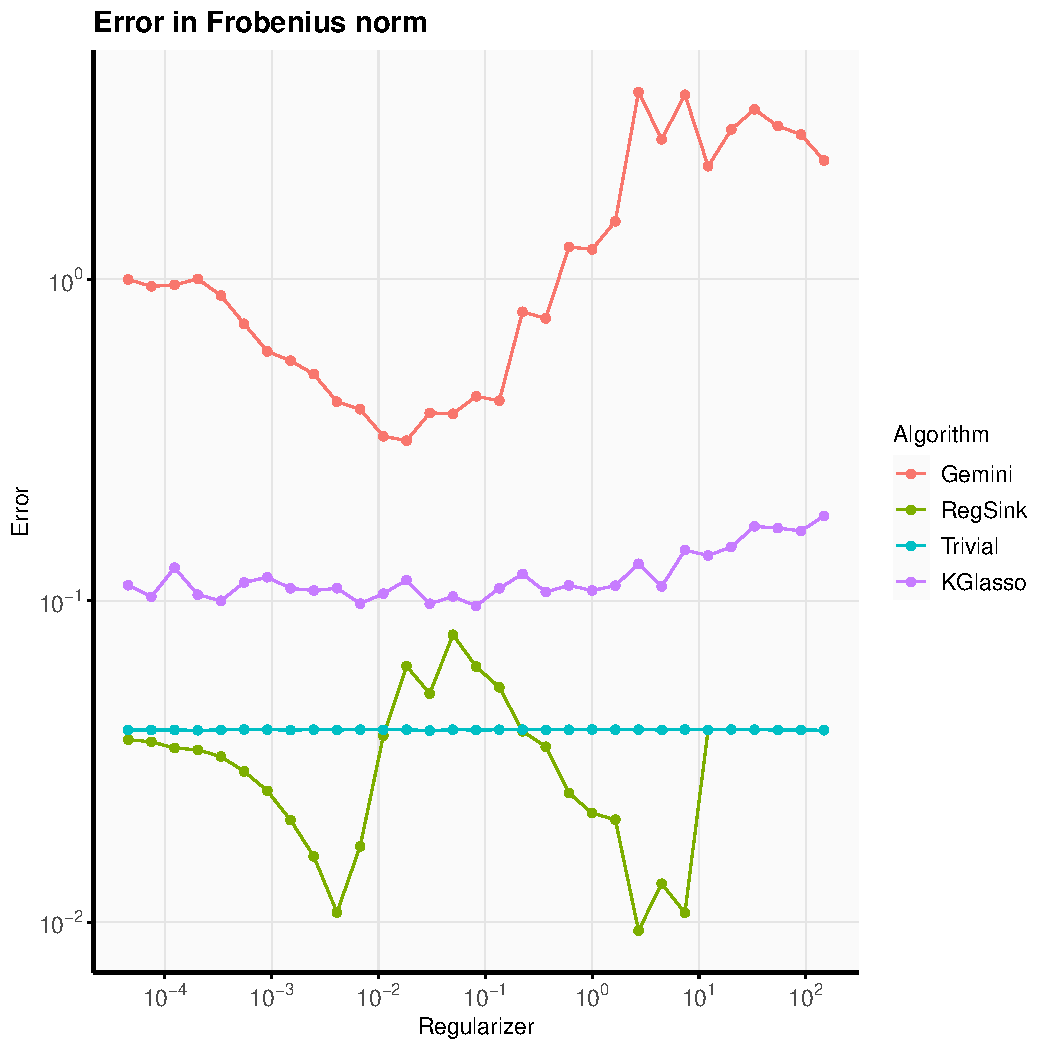
\includegraphics[width=\textwidth]{./code/zhou-comparison/25-50-spiked-frob.pdf}
         \end{subfigure}
          \begin{subfigure}[b]{.4\textwidth}
          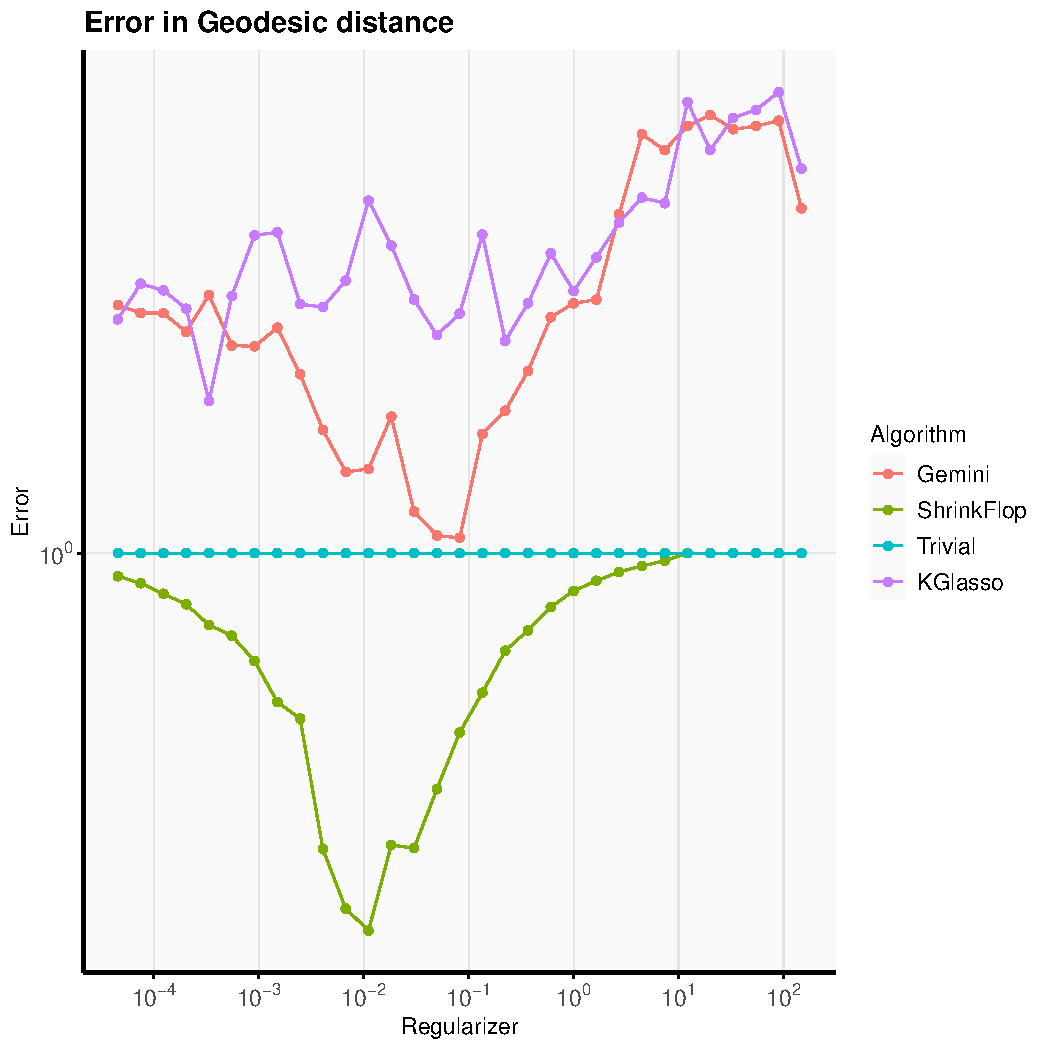
\includegraphics[width=\textwidth]{./code/zhou-comparison/25-50-spiked-geo.pdf}
          \end{subfigure}
         %\caption{$y=5/x$}
         %\label{fig:five over x}
        %\caption{Three simple graphs}
        %\label{fig:three graphs}
\caption{Average Frobenius error with $d_1 = 25, d_2 = 50, n = 1$ for spiked, dense covariance matrices. ``Gemini'' refers to the Gemini estimator of \cite{zhou2014gemini}, ``KGlasso'' refers to the Kronecker Glasso algorithm \cite{tsiligkaridis2013convergence}, ``ShrinkFlop'' refers to our shrinkage-based flip-flop estimator, and ``Trivial'' refers to the estimator that always outputs the identity matrix. The choice of regularizer~$\alpha$ for ShrinkFlop is given by $\alpha = \frac{2}{\pi} \arctan{x}$, where $x$ is the value on the $x$-axis in the figures above. }\label{fig:spiked}
\end{figure}

%-----------------------------------------------------------------------------
\subsection{Scenario 2: Sparse and partially sparse precision matrices}
%-----------------------------------------------------------------------------
%We next compare the performance of the estimator with Zhou's single step estimator \cite{zhou2014gemini} for the matrix normal model.
We now compare the performance of our estimator with other leading estimators in the case when one or more of the precision matrices $\Theta_1, \Theta_2$ is sparse. We find that when both $\Theta_1$ and $\Theta_2$ are sparse, the Gemini estimator outperforms the regularized Sinkhorn algorithm in Frobenius error; see \cref{fig:sparse-ii}. However, when $\Theta_2$ is spiked, we find that the shrinkage-based flip-flop estimator outperforms the Gemini estimator; see \cref{fig:sparse-i}. In practice, $\Theta_2$ is often considered a nuisance parameter and $\Theta_1$ is the object that should be interpretable (e.g., sparse). Thus ill-conditioned and dense nuisance parameters $\Theta_2$ can break GLASSO-type estimators even when $\Theta_1$ is sparse.

The figures were generated in the same manner as \cref{fig:spiked}, apart from the generative model. The sparse matrices $\Theta_i$ were generated by adding $\frac{1}{2}I_{d_1}$ to the Laplacian of a random multigraph with $0.4 d_i$ edges and normalizing to have trace $d_i$, and the spiked covariance matrix $\Sigma_2$ for \cref{fig:sparse-i} was drawn according to $\Sigma_2 \sim I_{d_2} + 100 v_2v_2^T$ where $v_2$ has i.i.d. Gaussian coordinates, and then normalized to have trace $d_2$.

\begin{figure}
              \centering
              \begin{subfigure}[b]{.4\textwidth}
         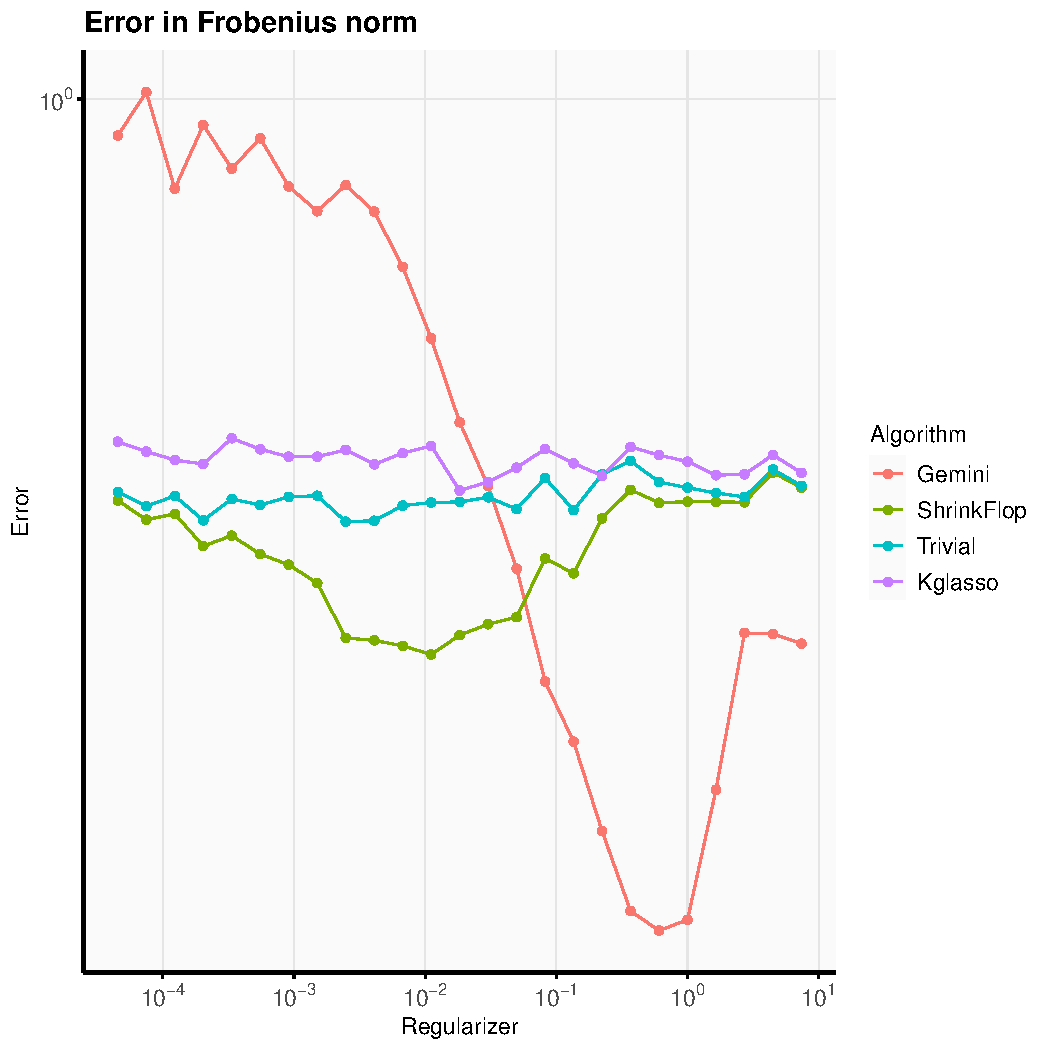
\includegraphics[width=\textwidth]{./code/zhou-comparison/25-50-doubly-sparse-frob.pdf}
         \end{subfigure}
         \begin{subfigure}[b]{.4\textwidth}
         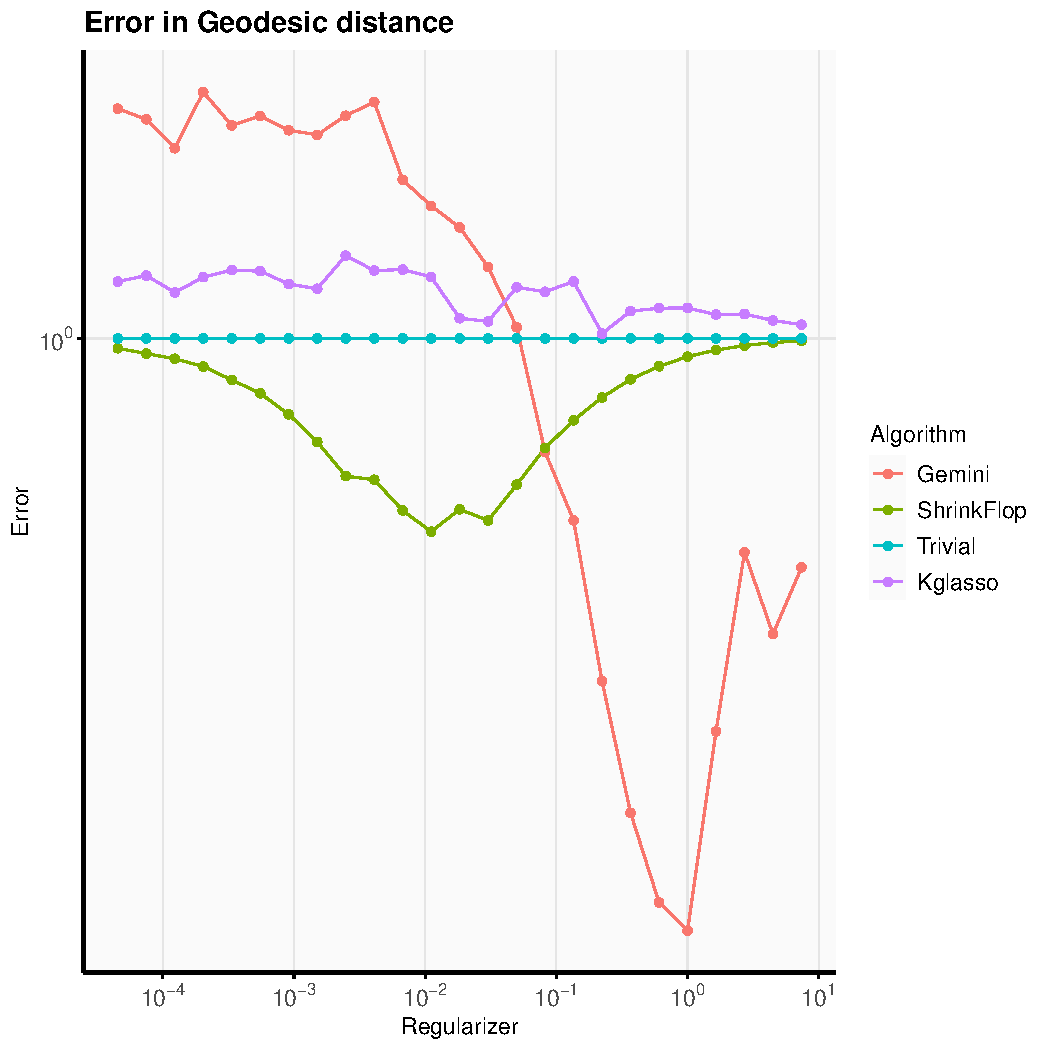
\includegraphics[width=\textwidth]{./code/zhou-comparison/25-50-doubly-sparse-geo.pdf}
         \end{subfigure}
         %\caption{$y=5/x$}
         %\label{fig:five over x}
        %\caption{Three simple graphs}
        %\label{fig:three graphs}
\caption{Average error with $d_1 = 25, d_2 = 50, n = 1$ for both precision matrices sparse.
Labels and choice of regularizer as in \cref{fig:spiked}.\label{fig:sparse-ii}}
\end{figure}


\begin{figure}
         \centering
                       \begin{subfigure}[b]{.4\textwidth}
         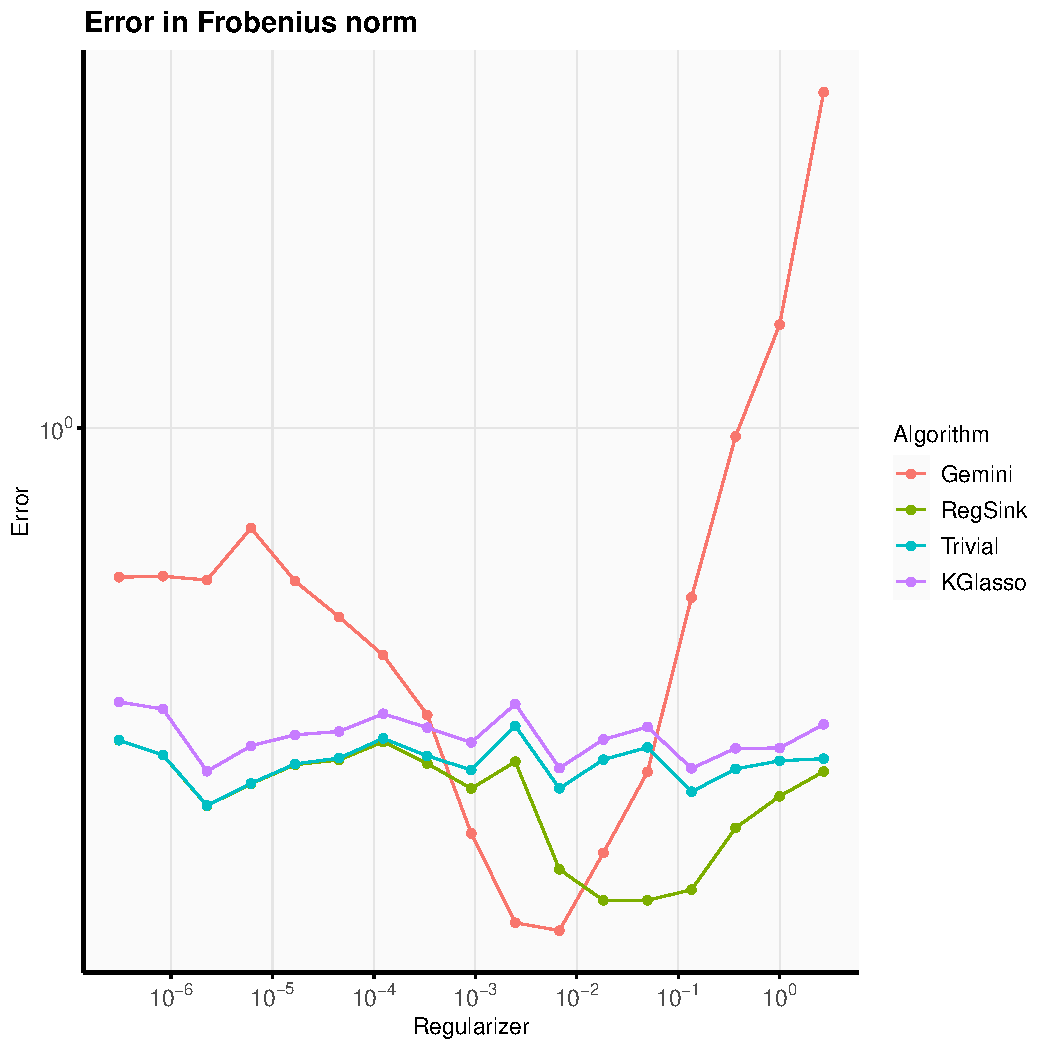
\includegraphics[width=\textwidth]{./code/zhou-comparison/25-50-sparse-frob.pdf}
         \end{subfigure}
         \begin{subfigure}[b]{.4\textwidth}
         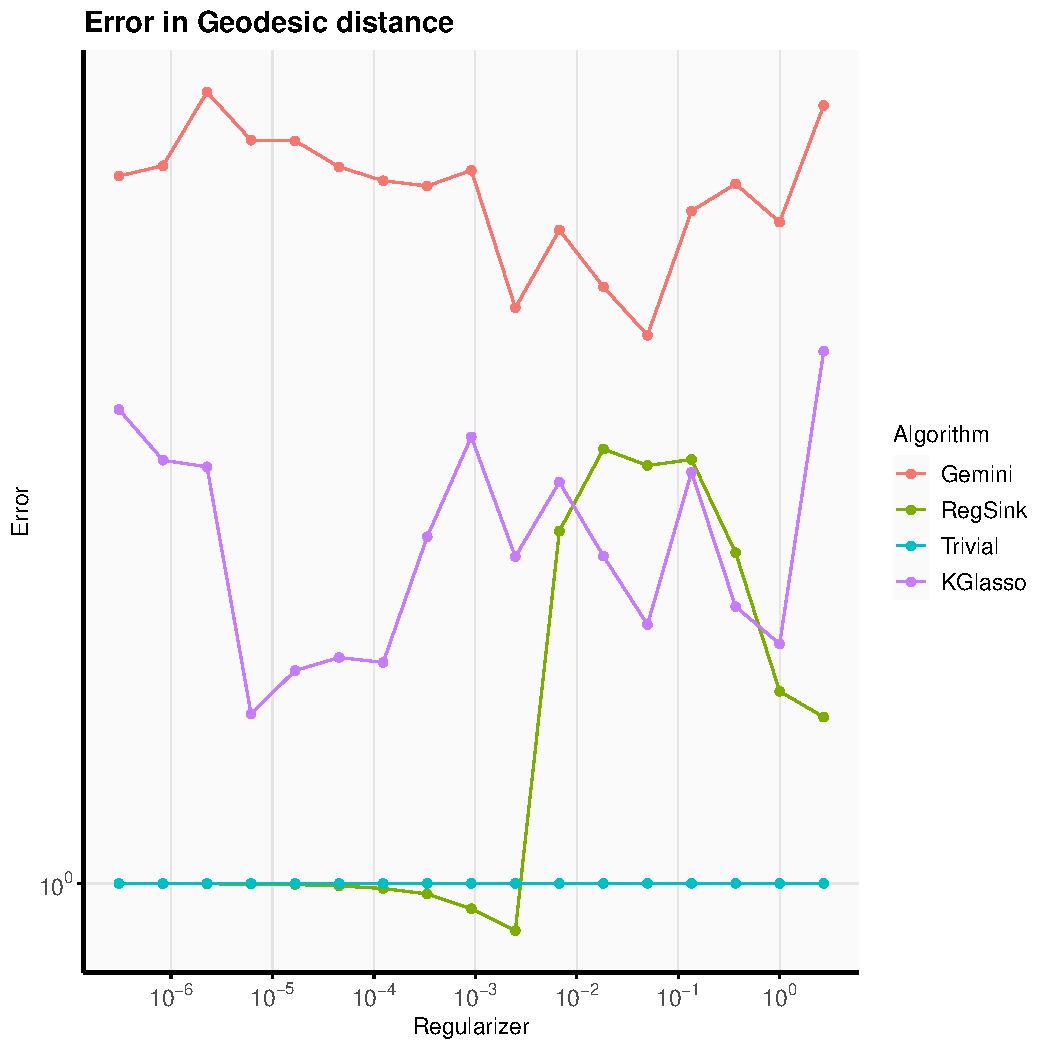
\includegraphics[width=\textwidth]{./code/zhou-comparison/25-50-sparse-geo.pdf}
         \end{subfigure}
         %\caption{$y=5/x$}
         %\label{fig:five over x}
        %\caption{Three simple graphs}
        %\label{fig:three graphs}
\caption{Average error with $d_1 = 25, d_2 = 50, n = 1$ for $\Theta_1$ sparse and $\Theta_2$ spiked. Interestingly, for Frobenius distance the shrinkage-based estimator performs best at the bottom of the regularization path and for the geodesic distance it performs best for larger regularization parameters.
Labels and choice of regularizer as in \cref{fig:spiked}.
\MW{What's going on with trivial in the RHS plot?}}\label{fig:sparse-i}
\end{figure}

%-----------------------------------------------------------------------------
\subsection{Performance as a function of the number of samples}
%-----------------------------------------------------------------------------
In this subsection we examine how the number of samples affects the error. We found best performance when the shrinkage parameter scales inverse exponentially with the number of samples, in this case $2^{-1.1 n}$. The regularization parameter for Gemini was chosen to scale as $\sqrt{(\log d_1) / d_2 n}$ as suggested in \cite{zhou2014gemini}.


In \cref{fig:lc} we see that Gemini outperforms flip-flop with a single sample, and shrinkage-based flip-flop outperforms both. When the number of samples are increased, the error for shrinkage-based flip-flop approaches that of flip-flop from below.


\begin{figure}
         \centering
                       \begin{subfigure}[b]{.4\textwidth}
         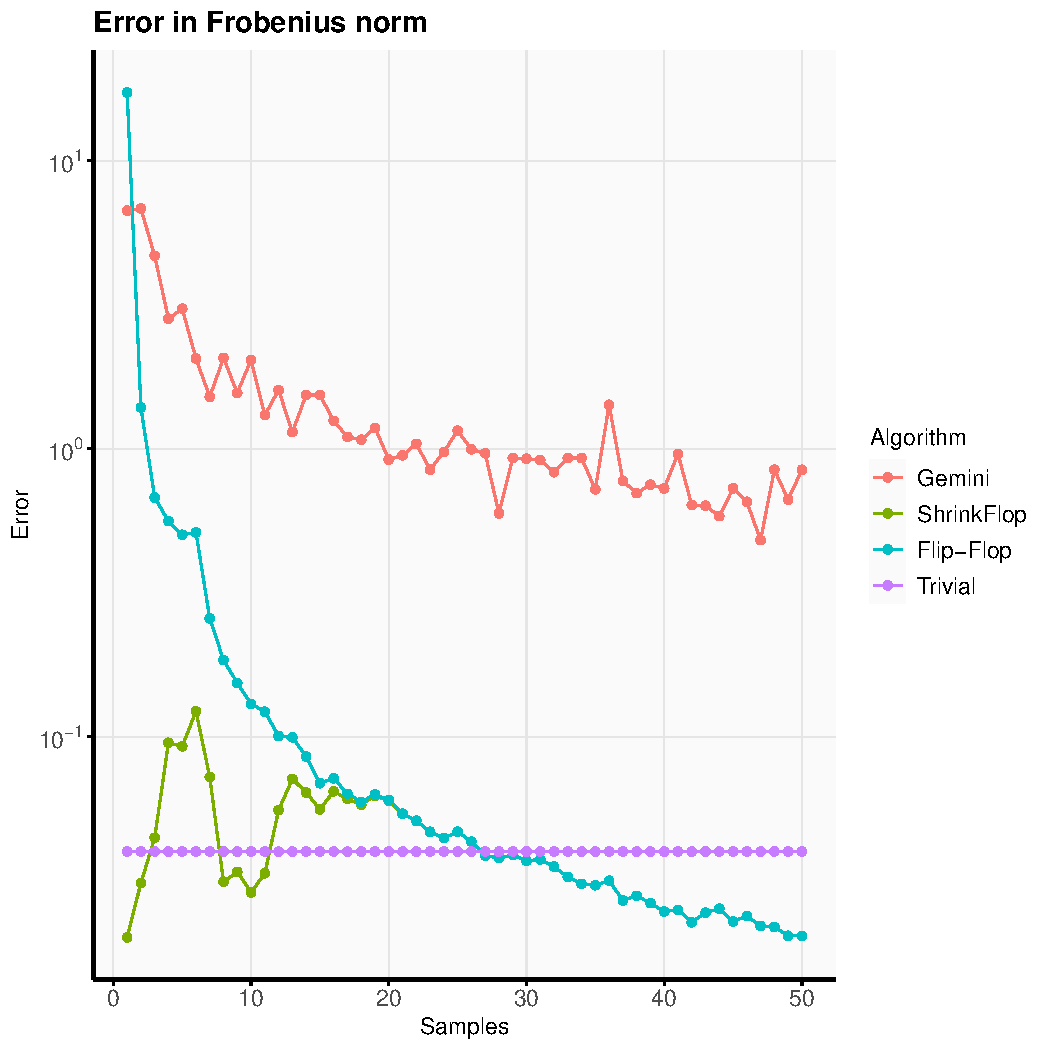
\includegraphics[width=\textwidth]{./code/zhou-comparison/25-25-spiked-lc-frob.pdf}
         \end{subfigure}
         \begin{subfigure}[b]{.4\textwidth}
         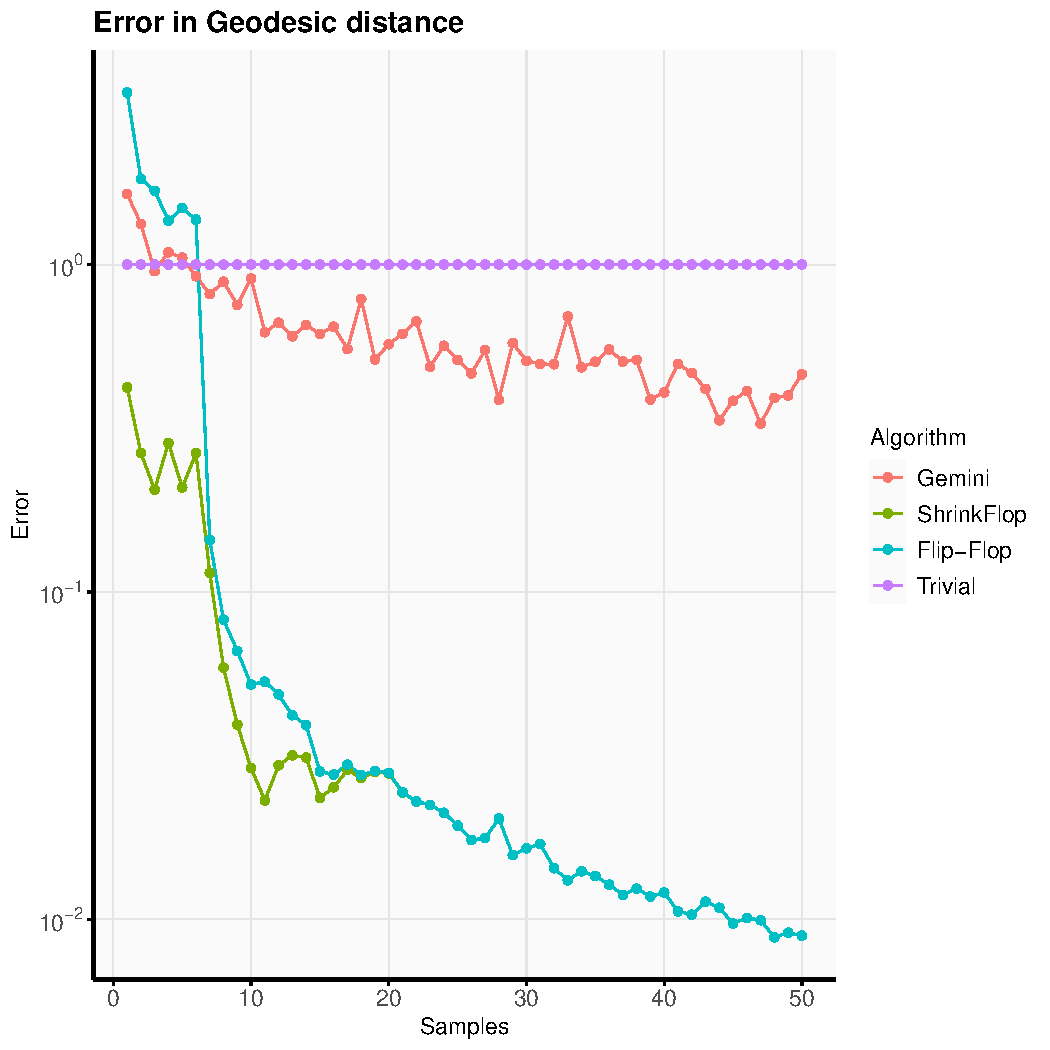
\includegraphics[width=\textwidth]{./code/zhou-comparison/25-25-spiked-lc-geo.pdf}
         \end{subfigure}
         %\caption{$y=5/x$}
         %\label{fig:five over x}
        %\caption{Three simple graphs}
        %\label{fig:three graphs}
\caption{Average error with $d_1 = 25, d_2 = 25, $ and number of samples $n$ ranging from $1$ to $50$ for both precision matrices spiked. It was necessary to choose $d_1 = d_2$ so that the flip-flop estimator converged for $n = 1$. We did not include KGlasso here because its running time was prohibitive. \MW{regularization for ShrinkFlop: $\alpha = 2^{-1.1n}$}\label{fig:lc}}
\end{figure}

%-----------------------------------------------------------------------------
\subsection{Computational aspects}
%-----------------------------------------------------------------------------
Here we experimentally demonstrate that our shrinkage-based estimator is much faster to compute than the Glasso-type estimators. We considered $d_1 =100, d_2 = 200$ with $n = 1$ samples. We considered regularized flip-flop and Gemini on spiked data, and chose the best regularization parameters for both using the computation from \cref{fig:spiked}. We did not consider KGLasso because it consistently took far longer than Gemini. Out of 2 draws of data from 2 instances, the average time of completion was 0.078 seconds for regularized flip-flop and 30 seconds for Gemini. Both computations were done in R using a MacBook~Pro with an Apple M1 chip with 16 gigabytes of RAM.

%=============================================================================
\section{Conclusion and open problems}
%=============================================================================
Though there has been a large volume of work on estimating the covariance in the matrix and tensor normal models under further assumptions like sparsity and well-conditionedness, some fundamental questions concerning estimation without further assumptions were still open prior to our work.
Contrary to the state of the art for unstructured covariance estimation (i.e., $k = 1$), all previous existing results depended on the condition number of the true covariance matrices (in the case of the tensor normal model under Frobenius norm) or had suboptimal sample complexity (the matrix normal model under operator norm).
Using strong convexity in the geometry induced by the Fisher information metric, we are largely able to remedy these issues and obtain nearly optimal estimates in the strongest possible metrics, namely the \emph{relative} operator and Frobenius norms.
As a consequence, we can also control other equivariant statistical distances such as relative entropy, Fisher-Rao distance, and total variation distance.

In particular, we showed that the maximum likelihood estimator (MLE) for the covariance matrix in the matrix normal models has optimal sample complexity up to logarithmic factors in the dimensions.
We showed that the MLE for tensor normal models with a constant number of tensor factors has optimal sample complexity in the regime where it is information-theoretically possible to recover the covariance matrix to within a constant Frobenius error.
Whenever the number of samples is large enough for either of the aforementioned statistical results to hold, we show that the flip-flop algorithm converges to the MLE exponentially quickly.
Hence, the output of the flip-flop algorithm with $O\left(\dmax +  \log n \right)$ \MW{still need to understand $\log n$ ;)} iterations is an efficiently computable estimator with statistical guarantees comparable to those we show for the MLE.

We also observed empirically that under a certain natural generative model of ill-conditioned, dense covariance matrices, the flip-flop algorithm combined with a very simple shrinkage technique can outperform existing estimators designed for the sparse case (Gemini and KGLASSO \MW{capitalization?}).
We view our empirical results as evidence that, in some cases, flip-flop combined with shrinkage provides the fastest, simplest and most statistically accurate known method to estimate the covariances.
More work is needed in the future to rigorously understand the statistical guarantees for flip-flop with shrinkage.


Our main theoretical open question is whether the assumption $n = \Omega( \dmax^3/ D)$ for \cref{thm:tensor-frobenius} can be weakened to $n = \Omega( \dmax^2/ D)$ for $k \geq 3$.
Equivalently, do the guarantees of \cref{thm:tensor-frobenius} hold even when one cannot hope to estimate the Kronecker factors to constant Frobenius error, but only to constant \emph{operator norm} error?
In the case $k = 1$ (i.e., unstructured covariance estimation) the weaker assumption is well-known to suffice, and for $k = 2$ the same follows (up to logarithmic factors) by our \cref{thm:matrix-normal}.
Filling in this final gap will place the tensor normal model on the same tight theoretical footing as unstructured covariance estimation.

\begin{appendix}

%=============================================================================
\section{Pisier's proof of quantum expansion}\label{sec:pisier}
%=============================================================================
In this appendix we prove the spectral condition for random Gaussian maps given in \cref{thm:hess-pisier}. 
This follows from the work of Pisier \cite{pisier2012grothendieck}, whose original theorem dealt with square matrices and gave slightly weaker probabilistic guarantees than \cref{thm:Pisier-expansion} stated below. We adapt this result to give exponentially small error probability in the setting of rectangular matrices. We emphasize that these are minor modifications which follow readily from \cite{P14} and \cite{pisier2012grothendieck}. Therefore, we state the proof below for completeness and claim no originality. 

\begin{theorem}[Pisier]\label{thm:Pisier-expansion}
Let $A_1,\dots,A_N,A$ be independent $n \times m$ random matrices with independent standard Gaussian entries.
For any~$t \geq 2$, with probability at least $1 - t^{-\Omega(m+n)}$,
\begin{align*}
  \norm*{\left(\sum_{i=1}^N A_i \otimes A_i \right) \circ \Pi}_{\op}
  \leq O\left( t^2 \sqrt{N} \bigl( \E \norm{A}_{\op} \bigr)^2 \right),
\end{align*}
where $\Pi$ denotes the orthogonal projection onto the traceless subspace of $\R^m \ot \R^m$, that is, onto the orthogonal complement of $\vect(I_m)$.
\end{theorem}

We first explain how \cref{thm:Pisier-expansion}, along with the following estimate of the operator norm of a standard Gaussian $n \times m$ random matrix~$A$ (see Theorem~5.32 in \cite{vershynin2010introduction}),
\begin{equation}\label{eq:op norm upper bound}
  \E \norm{A}_{\op} \leq \sqrt{n} + \sqrt{m},
\end{equation}
implies \cref{thm:hess-pisier}.

\begin{proof}[Proof of \cref{thm:hess-pisier}]
Choose $n=d_a$ and $m=d_b$.
Observe that
\begin{align*}
  \norm{\Phi_A}_0
= \max_{\substack{H \text{ traceless symmetric} \\ \norm H_F=1}} \norm{\Phi(H)}_F
% = \max_{\substack{H \text{ traceless symmetric} \\ \norm H_F \leq 1}} \norm{\Phi(H)}_F
\leq %\max_{\substack{H \in \Mat(n,m) \\ \norm H_F \leq 1}} \norm{\Phi(\Pi(H))}_F =
\max_{\substack{H \in \Mat(m) \\ \norm H_F = 1}} \norm{\Phi(\Pi(H))}_F
= \norm{\Phi \circ \Pi}_{\op}.
\end{align*}
Here we identified $\Mat(m) \cong \R^m \ot \R^m$, so $\Pi$ identifies with the orthogonal projection onto the traceless matrices, and we used that $\norm{\Pi(H)}_F \leq \norm{H}_F$, since $\Pi$ is an orthogonal projection.
Using \cref{eq:vec rep,thm:Pisier-expansion}, it follows that
\begin{align*}
  \norm{\Phi_A}_0 \leq O\left( t^2 \sqrt{N} \bigl( \E \norm{A}_{\op} \bigr)^2 \right),
\end{align*}
with the desired probability.
Using \cref{eq:op norm upper bound}, we can bound the right-hand side operator norm,
\begin{align*}
  \bigl( \E \norm{A}_{\op} \bigr)^2
= O\left( \left( \sqrt{n} + \sqrt{m} \right)^2 \right)
= O\left(n+m\right),
\end{align*}
which concludes the proof.
\end{proof}

In the remainder we discuss the proof of \cref{thm:Pisier-expansion}.
% Our setting required the result on rectangular matrices with strong error bounds \MW{$\leftarrow$ Should mention this at the beginning of the appendix instead of just talking about a `slightly different language'.}, so we follow the proof in \cite{pisier2012grothendieck} with these minor modifications and claim no originality.
The proof proceeds by a symmetrization trick, followed by the trace method.
We will first state a necessary concentration result and then give the proof of \cref{thm:Pisier-expansion}.

\begin{theorem}[Theorem~1.5 and~(1.3) in \cite{P86}]\label{thm:banach conc}
Let $A$ be a centered Gaussian random variable that takes values in a separable Banach space with norm $\|\cdot\|$.
Then $\|A\|$ satisfies the concentration and moment inequalities below with parameter $\sigma^2 := \sup \{ \E \langle \xi, A \rangle^{2} \mid \|\xi\|_{*} \leq 1 \}$, where $\|\cdot\|_{*}$ denotes the dual norm.
\[ \forall t > 0 \colon \quad \Pr\Bigl( \abs[\big]{\norm A - \E \norm A} \geq t\Bigr) \leq 2 \exp\Bigl( - \frac{\Omega(t^2)}{\sigma^{2}}\Bigr)  , \qquad \text{and}  \]
\begin{equation}\label{eq:conc via moments}
  \forall p \geq 2 \colon \quad (\E \|A\|^{p})^{\frac{1}{p}} \leq \E \|A\| + O \left( \sqrt{\frac{p}{\sigma^{2}}} \right).
\end{equation}
\MW{Not exactly the statement of the Lemma in Vershynin. $\norm A$ vs $\norm A - \E \norm A$, $p\geq1$ vs $p\geq 2$ -- but in particular the constant $\sigma$ should be in the numerator of \cref{eq:conc via moments}?}
\end{theorem}

\begin{remark}
The concentration inequalities and moment bounds in \cref{thm:banach conc} are related to the notion of sub-Gaussian random variables (see Lemma 5.5 of \cite{vershynin2010introduction}), and are often used in random matrix theory. 
\end{remark}

Below, we calculate the $\sigma^{2}$ parameter in \cref{thm:banach conc} with regards to our random matrix setting. 

\begin{corollary}\label{lem:opNormSubG}
Let $A$ be an $n \times m$ matrix with independent standard Gaussian entries.
Then $\norm{A}_{\op}$ is sub-Gaussian with parameter $\sigma^{2} = 1$. \MW{See sub-Gaussian comment above.}
\end{corollary}
\begin{proof}
Note that the dual norm is the trace norm~$\norm{\cdot}_{\operatorname{tr}}$, hence the concentration parameter can be estimated as
\begin{align*}
  \sigma^2
= \sup \left\{ \E \langle \xi, A \rangle^2 \;\mid\; \norm{\xi}_{\operatorname{tr}} \leq 1 \right\}
= \sup \left\{ \norm\xi_F^2 \;\mid\; \norm{\xi}_{\operatorname{tr}} \leq 1 \right\}
= 1,
\end{align*}
where we first used that $\braket{\xi,A}$ is distributed the same as $\norm\xi_F A_{11}$ by orthogonal invariance, and then that the trace norm dominates the Frobenius norm, with equality attained for example by $\xi = E_{11}$.
\end{proof}

We can now prove a lower bound that complements \cref{eq:op norm upper bound}.

\begin{lemma}\label{lem:op norm lower bound}
Let $A$ be an $n \times m$ matrix with independent standard Gaussian entries. Then there is some universal constant $c > 0$ such that
\begin{equation*}
  \E \norm{A}_{\op} \geq c (\sqrt{n} + \sqrt{m}).
\end{equation*}
\end{lemma}
\begin{proof}
% The moment definition of sub-Gaussianity from \cref{thm:banach conc} shows for $p=2$ and $\sigma^{2} = 1$ (by \cref{l:opNormSubG}) that
% \[
%   (\E \norm{A}_{\op}^{2})^{1/2} \leq \E \norm{A}_{\op} + C \sqrt{2}
% \implies \E \norm{A}_{\op} \geq (\E \norm{A}_{\op}^{2})^{1/2} - C \sqrt{2},
% \]
% where $C$ the universal constant in \cref{eq:conc via moments}.
% We can then lower bound the second moment
% \[ \E \norm{A}_{\op}^{2} = \E \norm{A^{T} A}_{\op} \geq \norm{\E A^{T} A}_{\op} = n ,  \]
% where the first step is by definition of $\norm{\cdot}_{\op}$, the second is by Jensen's inequality, and the third step is because $\E A^{T} A = n I_{m}$.
Without loss of generality we may assume that $n \geq m$.
Then,
\[ \E \norm{A}_{\op} \geq \E \norm{A e_{1}}_{2} \geq \frac{\sqrt{n}}{2} \geq \frac{\sqrt{m} + \sqrt{n}}{4}. \]
The second inequality follows by observing that $g := A e_1$ is a vector of standard Gaussian entries in~$\R^n$, so its length is distributed as $\E\sqrt X$ for $X = \norm g_2^2$ a chi-square variable with~$n$ degrees of freedom. This can be bounded by elementary integration (see Section 3.1 of \cite{ENormLB}).
\MW{I think this reference does not talk about chi-square random variables but rather asserts an explicit formula for this norm in terms of Gamma functions and the bounds $\frac n {\sqrt{n+1}} \leq \E\norm g_2 \leq \sqrt n$. Rephrase?}\CF{will track down akshay for this.} \AR{The reference just states elementary integration, so I thought I'd give a bit more intuition as to how I was able to see the result. }
\end{proof}

We will also use the the \emph{Schatten $p$-norm} $\norm{A}_p = (\tr\left[(A^TA)^{\frac p2}\right])^{\frac1p}$, which generalize the trace, Frobenius, and operator norms.
They satisfy the following H\"older inequality for $p\geq1$:
\begin{align}\label{eq:holder}
  \abs*{\tr \prod_{i=1}^{p} A_i} \leq \prod_{i=1}^{p} \norm{A_i}_p,
\end{align}

\begin{proof} [Proof of \cref{thm:Pisier-expansion}]
The operator we want to control has entries which are dependent in complicated ways.
We first begin with a standard symmetrization trick to linearize (compare the proof of Lemma~4.1 in~\cite{P14}).
A single entry of $A_i \otimes A_i$ is either a product $g g'$ of two independent standard Gaussians, or the square $g^2$ of a single standard Gaussian.
In expectation, we have $\E g g' = 0, \E g^{2} = 1$, and so the expected matrix is
\[ \E \left( \sum_{i=1}^N A_i \otimes A_i \right) = N \vect(I_n) \vect(I_m)^T. \]
Accordingly, after projection we have
\[ \E \left( \sum_{i=1}^N A_i \otimes A_i \right) \circ \Pi = 0. \]
Therefore we may add an independent copy:
Let $B_1,\dots,B_N$ be independent $n\times m$ random matrices with standard Gaussian entries, that are also independent from~$A_1,\dots,A_N$.
Then,
\begin{align*}
  \left( \sum_{i=1}^N A_i \otimes A_i \right) \circ \Pi
= \E_B \left( \sum_{i=1}^N A_i \otimes A_i - \sum_{i=1}^N B_i \otimes B_i \right) \circ \Pi
\end{align*}
and hence, for any $p\geq1$,
\begin{align*}
  \E \norm*{\left( \sum_{i=1}^N A_i \otimes A_i \right) \circ \Pi}_{\op}^p
\leq \E \norm*{\left( \sum_{i=1}^N A_i \otimes A_i - \sum_{i=1}^N B_i \otimes B_i \right) \circ \Pi}_{\op}^p
\end{align*}
by Jensen's inequality, as $\norm{\cdot}_{\op}^p$ is convex as the composition of the norm $\norm{\cdot}_{\op}$ with the convex and nondecreasing function $x \to x^{p}$.
Now note $(A_i,B_i)$ has the same distribution as $(\frac{A_i+B_i}{\sqrt2},\frac{A_i-B_i}{\sqrt2})$, so the right-hand side is equal to
\begin{align*}
&\quad \E \norm*{ \frac{1}{2} \left( \sum_{i=1}^N (A_i + B_i) \otimes (A_i + B_i) - \sum_{i=1}^N (A_i - B_i) \otimes(A_i - B_i) \right) \circ \Pi}_{\op}^p \\
&= \E \norm*{\left( \sum_{i=1}^N A_i \otimes B_i + \sum_{i=1}^N B_i \otimes A_i \right) \circ \Pi}_{\op}^p
% \leq 2 \E \norm*{\left( \sum_{i=1}^N A_i \otimes B_i \right) \circ \Pi}_{\op}^p
\leq 2^{p} \, \E \norm*{\sum_{i=1}^N A_i \otimes B_i}_{\op}^p
\end{align*}
Thus, we have proved that
\begin{align}\label{eq:symmetrization}
  \E \norm*{\left( \sum_{i=1}^N A_i \otimes A_i \right) \circ \Pi}_{\op}^p
\leq 2^{p} \, \E \norm*{\sum_{i=1}^N A_i \otimes B_i}_{\op}^p.
\end{align}
Note that we have lost the projection and removed the dependencies.
Next we use the trace method to bound the right-hand side of \cref{eq:symmetrization}.
That is, we approximate the operator norm by the Schatten $p$-norm for a large enough $p$ and control these Schatten norms using concentration of moments of Gaussians (compare the proof of Theorem~16.6 in~\cite{pisier2012grothendieck}).
For any $q\geq1$,
\begin{align*}
\E \norm*{\sum_{i=1}^N A_i \ot B_i}_{2q}^{2q}
% = \E \tr \left( \sum_{i=1}^N A_i \ot B_i \right)^{2q}
&= \E \tr \left[ \left( \sum_{i,j\in[N]} A_i^T A_j \ot B_i^T B_j \right)^{\!\!q} \, \right] \\
&= \sum_{i, j \in [N]^q} \E \tr \left( A^T_{i_1} A_{j_1} \cdots A^T_{i_q} A_{j_q} \ot B^T_{i_1} B_{j_1} \cdots B^T_{i_q} B_{j_q} \right) \\
&= \sum_{i, j \in [N]^q} \E \tr \left( A^T_{i_1} A_{j_1} \cdots A^T_{i_q} A_{j_q} \right) \E \tr \left( B^T_{i_1} B_{j_1} \cdots B^T_{i_q} B_{j_q} \right)
\end{align*}
where we used the independence of $\{A_i\}$ and $\{B_i\}$ in the last step.
Now, the expectation of a monomial of independent standard Gaussian random variables is always nonnegative.
% Now, the expectation of a (non-empty) monomial of independent standard Gaussian random variables vanishes unless each variable appears an even number of times, in which case it is positive.
Thus the same is true for $\E \tr ( A^T_{i_1} A_{j_1} \cdots A^T_{i_q} A_{j_q} )$, so we can upper bound the sum term by term as
\begin{align*}
&\quad \sum_{i, j \in [N]^q} \E \tr \left( A^T_{i_1} A_{j_1} \cdots A^T_{i_q} A_{j_q} \right) \E \tr \left( B^T_{i_1} B_{j_1} \cdots B^T_{i_q} B_{j_q} \right) \\
&\leq \sum_{i, j \in [N]^q} \E \tr \left( A^T_{i_1} A_{j_1} \cdots A^T_{i_q} A_{j_q} \right) \E \left( \norm{ B_{i_1} }_{2q} \norm{B_{j_1}}_{2q} \cdots \norm{ B_{i_q} }_{2q} \norm{B_{j_q}}_{2q} \right) \\
&\leq \sum_{i, j \in [N]^q} \E \tr \left( A^T_{i_1} A_{j_1} \cdots A^T_{i_q} A_{j_q} \right) \E \left( \norm{ B_1 }_{2q}^{2q} \right) \\
&= \left( \E\norm{\sum_{i=1}^N A_i}_{2q}^{2q} \right) \left( \E \norm{ A }_{2q}^{2q} \right)
= N^q \left( \E\norm{A}_{2q}^{2q} \right)^2.
\end{align*}
In the first step we used H\"older's inequality~\eqref{eq:holder} for the Schatten norm.
The second step holds since $\E\norm{B_i}_{2q}^k \leq (\E \norm{B_i}_{2q}^{2q})^{\frac k {2q}}$ by Jensen's inequality, so we can collect like terms together.
Next, we used that the~$B_i$ have the same distribution as $A$.
In the last step, we used that $\sum_i A_i$ has the same distribution as $\sqrt N A$.
Accordingly, we obtain for~$q\geq1$,
\begin{align*}
  \E \norm*{\sum_{i=1}^N A_i \ot B_i}_{2q}^{2q}
\leq N^q \left( \E\norm{A}_{2q}^{2q} \right)^2,
\end{align*}
and hence
\begin{align*}
\E \norm*{\left( \sum_{i=1}^N A_i \otimes A_i \right) \circ \Pi}_{\op}^{2q}
&\leq 4^q \, \E \norm*{\sum_{i=1}^N A_i \ot B_i}_{\op}^{2q}
\leq 4^q \, \E \norm*{\sum_{i=1}^N A_i \ot B_i}_{2q}^{2q} \\
&\leq (4N)^q \left( \E\norm{A}_{2q}^{2q} \right)^2
\leq (4N)^q m^2 \Bigl( \E\norm{A}_{\op}^{2q} \Bigr)^2.
\end{align*}
The first inequality is \cref{eq:symmetrization}, and in the last inequality we used that $A \in \Mat(n,m)$ has rank~$\leq m$, and therefore $\norm{A}_{2q}^{2q} \leq m \norm A_{\op}^{2q}$.
To bound the right-hand side, we use \cref{thm:banach conc}, applied to the random variable~$A$ in the Banach space~$\Mat(n,m)$ with the operator norm~$\norm{\cdot}_{\op}$.
Then, $\sigma^2=1$, as computed in \cref{lem:opNormSubG}, and we find that
\begin{align*}
\E \norm*{\left( \sum_{i=1}^N A_i \otimes A_i \right) \circ \Pi}_{\op}^{2q}
\leq (4 N)^q m^2 \Bigl( \E\norm A_{\op} + C \sqrt{q} \Bigr)^{4q}.
\end{align*}
where~$C>0$ is a universal constant implied by the big-$O$ notation in \cref{eq:conc via moments}.
Finally, we can use Markov's inequality to see that, for some large universal constant $C' \geq 1$ that we choose later, the event
\begin{align}\label{eq:desired event}
  \norm*{\left(\sum_{i=1}^N A_i \otimes A_i \right) \circ \Pi}_{\op}
  \leq (C' t)^2 \sqrt{4 N} \bigl( \E \norm{A}_{\op} \bigr)^2
\end{align}
holds up to failure probability at most
\begin{align*}
  \frac{\E \norm*{\left(\sum_{i=1}^N A_i \otimes A_i \right) \circ \Pi}_{\op}^{2q}}{\left( (C' t)^2 \sqrt{4 N} \bigl( \E \norm{A}_{\op} \bigr)^2 \right)^{2q}}
\leq % \frac{2 N^q m^2 \Bigl( \E\norm A_{\op} + C \sqrt{q} \Bigr)^{4q}}{(2C')^{4q} t^{4q} N^q \bigl( \E \norm{A}_{\op} \bigr)^{4q}} =
  % \frac{m^2 \Bigl( \E\norm A_{\op} + C \sqrt{q} \Bigr)^{4q}}{(C' t)^{4q} \bigl( \E \norm{A}_{\op} \bigr)^{4q}}.
  % \frac{m^2 \Bigl( \E\norm A_{\op} + C \sqrt{q} \Bigr)^{4q}}{\bigl( C' t \, \E \norm{A}_{\op} \bigr)^{4q}}.
  m^2 \left( \frac{\E\norm A_{\op} + C \sqrt{q}}{C' t \, \E \norm{A}_{\op}} \right)^{4q}.
\end{align*}
We choose $q = \max\{1, (C^{-1} \E \norm{A}_{\op})^{2} \}$, which by \cref{lem:op norm lower bound} is $\Omega(m + n)$.
We now have two cases.
If $\E \norm{A}_{\op} \leq C$, and therefore $q = 1$, then we can bound the failure probability as
\begin{align*}
  m^2 \left( \frac{\E\norm A_{\op} + C \sqrt{q}}{C' t \, \E \norm{A}_{\op}} \right)^{4q}
\leq m^2 \left( \frac{2C}{C' t \, \E \norm{A}_{\op}} \right)^{4q}
\leq m^2 t^{-4q},
\end{align*}
where the second inequality follows by choosing $C'$ large enough, as $\E\norm A_{\op}$ is bounded below by a universal constant (according to \cref{lem:op norm lower bound}).
If instead $C \sqrt{q} \leq \E \norm{A}_{\op}$, then we bound the failure probability as
\begin{align*}
  m^2 \left( \frac{\E\norm A_{\op} + C \sqrt{q}}{C' t \, \E \norm{A}_{\op}} \right)^{4q}
\leq m^2 \left( \frac{2 \E\norm A_{\op}}{C' t \, \E \norm{A}_{\op}} \right)^{4q}
= m^2 \left( \frac{2}{C' t} \right)^{4q}
\leq m^2 t^{-4q}
\end{align*}
where the seond inequality follows by choosing~$C'\geq2$.
Thus, in either case the event~\eqref{eq:desired event} holds up to a failure probability of at most
\begin{align*}
  m^2 t^{-4q} = t^{-\Omega(m+n)},
\end{align*}
where we used that $q = \Omega(m + n)$ as well as the fact that $t\geq2$, so the prefactor $m^{2}$ can be absorbed at the cost of slightly changing the constant in the exponent.
\end{proof}


%=============================================================================
\section{Proof of the robustness lemma}\label{app:robust}
%=============================================================================
\CF{Read appendix B.}
In this appendix we give a proof of \cref{convexRobustness}, which shows that strong convexity at a particular point implies strong convexity nearby.
First note that by \cref{remark:hessian-everywhere}, we have $\nabla^2 f_\samp(\Theta) = \nabla^2 f_{\samp'}$ where $\samp' = \Theta^{1/2} \samp$.
Thus we need only bound the difference between $f_\samp$ and $f_{\samp'}$ for $\|\log \Theta\|_{\op}$ small, $\Theta \in \P$.
For a matrix $\delta$ in $\Mat(d_a)$, we adopt the abuse of notation
$$e^{\delta_{(a)}} = I_{d_1} \otimes \cdots \otimes I_{d_{a-1}} \otimes e^{\delta} \otimes I_{d_{a+1}} \otimes \cdots \otimes I_{d_k}.$$
We will write $\Theta^{1/2}$ as $e^{\delta}$, where $\delta = \sum_{a =1}^k \delta_{(a)}$.
\MW{$\leftarrow$ $\delta$ is already a matrix in $\Mat(d_a)$, now it is a matrix tuple}
We now have $\Theta^{1/2} = e^{\delta} = \otimes_{a = 1}^k e^{\delta_a}$, and $\frac{1}{2}\|\log \Theta\|_{\op} = \|\delta\|_{\op} = \sum_{a =1}^k \|\delta_{a}\|_{\op}$.
To bound the difference between $\nabla^2 f_{x'}$ and $\nabla^2 f_x$, we will show each component of the Hessian $\nabla f_{x'}$ (as presented in \cref{lem:hessian}) only changes (from $\nabla f_x$) by a small amount under the perturbation $x' := e^\delta x \leftarrow x$.
In particular we will give bounds on each block under each component-wise perturbation $e^{\delta_{(a)}}x \leftarrow x$, and write the overall perturbation as a sequence of such component-wise perturbations. For convenience, we adopt the short-hand
$$ \rho_x:= \frac{1}{nD} x x^T.$$



We begin with an easy fact relating the exponential map and the operator norm.

\begin{fact} \label{f:expTaylor} For all symmetric $d\times d$ matrices $A$ such that $ \|A\|_{\op} \leq 1$, we have
$$ \|e^{A} - I\|_{\op} \leq 2 \|A\|_{\op}.$$
\end{fact}


%Recall the definition of a quadratic form of the Hessian:
%\[ \langle Z, (\nabla^{2} f) Z \rangle = \langle Z, (\nabla^{2} F) Z \rangle + \langle Z, (\nabla^{2} f - \nabla^{2} F) Z \rangle     \]
%The second term is rank one, so the quadratic form is:
%\[ \langle Z, (\nabla^{2} f - \nabla^{2} F) Z \rangle = \left( \sum_{a} \sqrt{d_{a}} \langle \rho^{(a)}, Z_{a} \rangle   \right)^{2}       \]
\noindent The $00$ component of the Hessian is a scalar $\nabla^{2}_{00} f = \tr[\rho]$, and for $a \geq 1$ we think of each $0a$ component as a vector:
\[ \sum_{a} \langle z_{0}, (\nabla^{2}_{0a} f) Z_{a} \rangle = z_{0} \langle \rho, \sum_{a} \sqrt{d_{a}} Z_{(a)} \rangle       \]
The diagonal components involve only one-body marginals of $\rho$:
\[ \langle Z_{a}, (\nabla^{2}_{aa} f) Z_{a} \rangle = \langle d_{a} \rho^{(a)}, Z_{a}^{2} \rangle       \]
And the off-diagonal components involve two-body marginals:
\[ \langle Z_{a}, (\nabla^{2}_{ba} f) Z_{b} \rangle =  \langle \sqrt{d_{a} d_{b}} \rho^{(ab)}, Z_{a} \otimes Z_{b} \rangle.   \]
Therefore in \cref{atoaaRobustness} and \cref{btoaaRobustness}, we will prove perturbation bounds on one-body marginals, and in \cref{btoabRobustness} we will prove perturbation bounds on two-body marginals. This will allow us to bound the change in the $0a$ components, diagonal components, and the off-diagonal components, respectively.
Then, following the structure of the proof of \cref{thm:tensor-convexity}, we will collect all the term-wise bounds to prove an overall bound at the end of the section.


%By the above discussion then we will bound the difference of each under each component-wise perturbation. Note the terms involve $\{\rho^{(a)}\}, \{\rho^{(ab)}\}$, so we prove perturbations on marginals in the following lemmas.

\begin{lemma} \label{atoaaRobustness}
For $\samp \in \R^{D \times n}$ and a symmetric matrix $\delta \in \Mat(d_{a})$ such that $\|\delta\|_{\op} \leq 1$, if we denote $\samp' := e^{\delta_{(a)}} \samp$ then
\[ \|\rho_{\samp'}^{(a)} - \rho_{\samp}^{(a)}\|_{\op} \leq 8 \|\delta\|_{\op} \|\rho_{\samp}^{(a)}\|_{\op}   . \]
\end{lemma}
\begin{proof}By definition, $\|\rho_{\samp'}^{(a)} - \rho_{\samp}^{(a)}\|_{\op} = \sup_{\|Z\|_{1} \leq 1} \langle Z_{(a)}, \rho_{\samp'} - \rho_{\samp} \rangle $.
Let $\delta' := e^{\delta} - I_{a}$. Note that $\|\delta'\|_{\op} \leq 2 \|\delta\|_{\op}$ by \cref{f:expTaylor} and our assumption $\|\delta\|_{\op} \leq 1$. Now
\begin{align*} \langle Z_{(a)}, \rho_{\samp'} - \rho_{\samp} \rangle &= \langle Z_{(a)}, (I+\delta')_a \rho_{\samp} (I+\delta')_a - \rho_{\samp} \rangle \\
& = \langle Z, \delta' \rho_\samp^{(a)} \rangle + \langle Z, \rho_\samp^{(a)} \delta' \rangle + \langle Z, \delta' \rho_\samp^{(a)} \delta' \rangle \\
& \leq (2\|\delta'\|_{\op} + \|\delta'\|_{\op}^{2}) \|\rho^{(a)}\|_{\op}\|Z\|_1  \\
&\leq 8 \|\delta\|_{\op} \|\rho^{(a)}\|_{\op}.\end{align*}
\end{proof}

%\CF{ I think we should combine these lemmas into a single one with two items.}\AR{The proofs are different, and I like the similar structure for diagonal/off-diagonal blocks. It may clutter the statements more to combine. }
\begin{lemma} \label{btoaaRobustness}
For $\samp \in \R^{D \times n}$ and symmetric matrix $\delta \in \Mat(d_{b})$ such that $\|\delta\|_{\op} \leq 1$, if we denote $\samp' := e^{\delta_{(b)}} \samp$ then for $b \neq a$:
\[ \|\rho_{\samp'}^{(a)} - \rho_{\samp}^{(a)}\|_{\op} \leq 2 \|\delta\|_{\op} \|\rho_{\samp}^{a}\|_{\op} .    \]
\end{lemma}
\begin{proof}
By definition, $\|\rho_{\samp'}^{(a)} - \rho_{\samp}^{(a)}\|_{\op} = \sup_{\|Z\|_{1} \leq 1, Z \succeq 0} |\langle Z_{(a)}, \rho_{\samp'} - \rho_{\samp} \rangle|$. \\
Let $\delta' := e^{\delta} - I_b$.
Note that $\|\delta'\|_{\op} \leq 2 \|\delta\|_{\op}$ by \cref{f:expTaylor} and our assumption $\|\delta\|_{\op} \leq 1$. \\
Now
\begin{align*}
|\langle Z_{(a)}, \rho_{\samp'} - \rho_{\samp} \rangle|
& = | \langle Z_{(a)}, e^{\delta_{(b)}}\rho_{\samp} e^{\delta_{(b)}} - \rho_{\samp} \rangle|\\
& = | \langle Z_{(a)} \delta'_{(b)}, \rho_{\samp} \rangle   |
= | \langle Z \otimes \delta', \rho_{\samp}^{(ab)} \rangle   | \\
% &\leq \langle Z \otimes |\delta_b'|, \rho_{\samp}^{(ab)} \rangle\\
&\leq \langle \|\delta'\|_{\op} Z \otimes  I_b , \rho_{\samp}^{(ab)} \rangle\\
&= \|\delta'\|_{\op} \langle Z, \rho_{\samp}^{(a)} \rangle \leq 2\|\delta\|_{\op} \|Z\|_1 \|\rho_{\samp}^{(a)}\|_{\op}.
\end{align*}
\end{proof}



This is already enough to prove a bound on $0a$ and $aa$ terms:
%and rank one term $(\nabla^{2} f - \nabla^{2} F)$.

\begin{corollary} \label{diagRobustness}
Let $\samp \in \R^{D \times n}$ be such that $\|d_{a} \rho_{\samp}^{(a)}\|_{\op} \leq 1 + \frac{1}{20}$, and for $b \in [k]$ let $\delta_b \in \Mat(d_b)$ be a  symmetric matrix such that $\sum_{b} \|\delta_{b}\|_{\op} \leq \frac{1}{8}$. Denoting $\delta_{(b)} := (\delta_b)_{(b)}$,  $\delta = \sum_b \delta_{(b)}$ and $x' = e^{\delta} \samp$, for $a \geq 1$ we have
\[ \|\nabla^{2}_{aa} f(e^{2\delta}) - \nabla^{2}_{aa} f(I)\|_{\op} \leq 25 \|\delta\|_{\op} .  \]

\end{corollary}
%\CF{technically $f(e^{\delta})$ corresponds to $e^{\delta/2} \samp$}
\begin{proof}
Recall from \cref{lem:hessian} that $\langle Y, (\nabla^{2}_{aa} f_{\samp}) Y \rangle = \langle d_{a} \rho_{\samp}^{(a)}, Y^{2} \rangle$; thus it is enough to show that $\|\rho_{\samp'}^{(a)} - \rho_{\samp}^{(a)}\|_{\op} \leq 25 \|\delta\|_{\op} /d_a$. We treat the perturbation $e^\delta$ as the composition of $k$ perturbations:
\[ \samp_{(0)}:=\samp \to \samp_{(1)}:= e^{\delta_{(1)}} \samp_{(0)} \to ... \to \samp_{(k)}:=e^{\delta_{(k)}} \samp_{(k-1)} = \samp'. \]
We can use \cref{atoaaRobustness} to handle $e^{\delta_{(a)}}$ and \cref{btoaaRobustness} for the rest. Let $Z$ be a symmetric matrix.
\begin{align*}
 |\langle \rho_{\samp'}^{(a)} - \rho_{\samp}^{(a)}, Z \rangle|
 &\leq \sum_{j=1}^{k} |\langle \rho_{\samp_{(j)}}^{(a)} - \rho_{\samp_{(j-1)}}^{(a)}, Z \rangle| \\
 &\leq \sum_{j=1}^{k}  8 \|\delta_{j}\|_{\op} \|\rho_{\samp_{(j-1)}}^{(a)}\|_{\op} \|Z\|_{1}.
\end{align*}
Where the last inequality is due to \cref{atoaaRobustness,btoaaRobustness}.
To bound each term in the right-hand side, note that by \cref{atoaaRobustness,btoaaRobustness} we have
$$\|\rho_{\samp_{(j)}}^{(a)}\|_{\op} \leq \|\rho_{\samp_{(j)}}^{(a)} - \rho_{\samp_{(j-1)}}^{(a)}\|_{\op} + \|\rho_{\samp_{(j-1)}}^{(a)}\|_{\op} \leq   (1+8 \|\delta_{j}\|_{\op})\|\rho_{\samp_{(j-1)}}^{(a)}\|_{\op}$$
and hence by induction the $j^{th}$ term in the sum is at most $$8 \|\delta_j\|_{\op} \left( \prod_{l=1}^k (1+8 \|\delta_{l}\|_{\op}) \right) \|\rho_{\samp}^{(a)}\|_{\op} \|Z\|_{1}.$$ By our assumption that $\sum_l \|\delta_l\|_{\op} \leq 1/8$, this is at most $8 \|\delta_j\|_{\op} e^{8 \sum \|\delta_l\|_{\op}} \|\rho_{\samp}^{(a)}\|_{\op} \|Z\|_{1} \leq 8e \|\delta_j\|_{\op} \|\rho_{\samp}^{(a)}\|_{\op} \|Z\|_{1}. $ Adding up the terms and using that $\|\delta\|_{\op} = \sum \|\delta_{(c)}\|_{\op}$, the overall sum is then at most $8 e \|\delta\|_{\op} \|\rho_{\samp}^{(a)}\|_{\op} \|Z\|_{1}$. Using our assumption on $\|d_{a} \rho_{\samp}^{(a)}\|_{\op}$ completes the proof.
\end{proof}

\begin{corollary} \label{constantRobustness}
Let $\samp \in \R^{D \times n}$ be such that $\|d_{a} \rho_{\samp}^{(a)}\|_{\op} \leq 1 + \frac{1}{20}$, and for $b \in [k]$ let $\delta_b$ be symmetric matrices such that $\|\sum_{b} \delta_{(b)}\|_{\op} = \sum_{b} \|\delta_{b}\|_{\op} \leq \frac{1}{8}$, where once again we denote $\delta_{(b)} := (\delta_b)_{(b)}$ and $\delta := \sum_b \delta_{(b)}$.
Denoting $\samp' := e^{\delta} \samp$, for $a \geq 1$ we have
\begin{align*} |\nabla^{2}_{00} f_{\samp'} - \nabla^{2}_{00} f_{\samp}| &\leq 5 \|\delta\|_{\op}  \\
\text{ and } \|\nabla^{2}_{0a} f_{\samp'} - \nabla^{2}_{0a} f_{\samp}\|_{\op} &\leq 25 \|\delta\|_{\op} .  \end{align*}
\end{corollary}
\begin{proof}
Recall from \cref{lem:hessian} that the $00$ component of the Hessian is just the scalar $\tr \rho$. The assumption that $\|d_{a} \rho_{\samp}^{(a)}\|_{\op} \leq 1 + \frac{1}{20}$ implies $\tr[\rho_{\samp}] = \tr \rho_{\samp}^{(a)} \leq 1 + 1/20$. Now we can use the approximation for $e^{\delta}$ in \cref{f:expTaylor}:
\[ |\tr[\rho_{\samp'} - \rho_{\samp}]| = |\langle \rho_{\samp}, e^{2\delta} - I \rangle| \leq \tr[\rho_{\samp}] \|e^{2 \delta} - I\|_{\op} \leq 5 \|\delta\|_{\op}     \]
In the last step we used our bound on $\tr[\rho_{\samp}].$
The $0a$ component is a vector, so it is enough to bound the inner product with any traceless matrix $Z$ of unit Frobenius norm:
\[ |\langle \rho_{\samp'}^{(a)} - \rho_{\samp}^{(a)}, \sqrt{d_{a}} Z \rangle| \leq \|\rho_{\samp'}^{(a)} - \rho_{\samp}^{(a)}\|_{\op} \sqrt{d_{a}} \|Z\|_{1}. \]
In the proof of \cref{diagRobustness} we showed under the same assumptions we have $\|\rho_{\samp'}^{(a)} - \rho_{\samp}^{(a)}\|_{\op} \leq 25 \|\delta\|_{\op}/d_a$, from which it follows that the above is at most $25 \|\delta\|_{\op} \|Z\|_{F}.$ \end{proof}

%\begin{corollary} \label{rankoneRobustness}
%For input $x \in \R^{nD}$ such that for all $a \in [k]$ such that $\|d_{a} \rho_{\samp}^{(a)} - \tr[\rho_{\samp}] I_{a}\|_{\op} \leq \frac{1}{20}$; and perturbation $\delta := \sum_{a} (\delta_{a} \in \Mat(d_{a}))_{a}$ such that $\|\delta\|_{\op} = \sum_{a} \|\delta_{a}\|_{\op} \leq \frac{1}{20}$; if we denote $\samp' := e^{\delta} \samp$, then we have:
%\[ \|(\nabla^{2} f_{\samp'} - \nabla^{2} F_{\samp'}) - (\nabla^{2} f_{\samp} - \nabla^{2} F_{\samp})\|_{\op} \leq 1.5 k \|\delta\|_{\op}     \]
%\end{corollary}
%\begin{proof}
%Recall again from the discussion after $\cref{convexRobustness}$ that $\langle Z, (\nabla^{2} F - \nabla^{2} f) Z \rangle = \left\langle \rho, \sum_{a} \sqrt{d_{a}} (Z_{a})_{a}  \right\rangle^{2}$. We use the same iterative strategy as $\cref{diagRobustness}$:
%\[    \left\langle \rho_{\samp'}, \sum_{a} \sqrt{d_{a}} (Z_{a})_{a}  \right\rangle^{2} -  \left\langle \rho_{\samp}, \sum_{a} \sqrt{d_{a}} (Z_{a})_{a}  \right\rangle^{2}    \]
%\[ = \left\langle \rho_{\samp'} + \rho_{\samp}, \sum_{a} \sqrt{d_{a}} (Z_{a})_{a}  \right\rangle \left\langle \rho_{\samp'} - \rho_{\samp}, \sum_{a} \sqrt{d_{a}} (Z_{a})_{a}  \right\rangle  \]
%\[ = \left( \sum_{a} \langle (d_{a} \rho_{\samp'}^{(a)} - \tr[\rho_{\samp'}] I_{a}) + (d_{a} \rho_{\samp}^{(a)} - \tr[\rho_{\samp}] I_{a}) , d_{a}^{-1/2} Z_{a} \rangle \right) \left( \sum_{a} \sqrt{d_{a}} \langle \rho_{\samp'}^{(a)} - \rho_{\samp}^{(a)}, Z_{a} \rangle \right)     \]
%%\AR{Here I could use that $Z \perp I$ to get a constant factor improvement; need an assumption on $\nabla$; but it improves the overall constant by factor $\approx 2$}
%\[ \leq \left( \sum_{a} (2 + 10 \|\delta\|_{\op}) \|d_{a} \rho_{\samp}^{(a)} - \tr[\rho_{\samp}] I_{a} \|_{\op} \|d_{a}^{-1/2} Z_{a}\|_{1}   \right)
%\left( 10\|\delta\|_{\op} \sum_{a} \sqrt{d_{a}} \| \rho_{\samp}^{(a)}\|_{\op} \|Z_{a}\|_{1}   \right)    \]
%\[ \leq \left( \sum_{a} \frac{2 + 10 \|\delta\|_{\op}}{20} \|Z_{a}\|_{F}  \right)
%\left( 10\|\delta\|_{\op} \sum_{a} (1 + \frac{1}{20}) \|Z_{a}\|_{F} \right)
%\leq 1.5 k \|\delta\|_{\op} \|Z\|^{2}      \]
%%\AR{What norm are we using on $Z$ as a whole? Should I keep around the $d_{a}$'s?} \CF{the norm is just the standard norm, there shouldn't be $d_a$'s}
%% The final step follows from the initial conditions on $\|d_{a} \rho_{a}\|_{\op}, \|d_{b} \rho_{b}\|_{\op}$.
%In the third line we used that $Z$ is traceless; in the last line we used our initial conditions on $\rho$; the last step was by Cauchy-Schwarz.
%\end{proof}


The off-diagonal components require the following two lemmata on bipartite marginals:

\begin{lemma} \label{btoabRobustness}
For $\samp \in \R^{D \times n}$ and a symmetric matrix $\delta \in \Mat(d_{c})$ such that $\|\delta\|_{\op} \leq \frac{1}{8}$; if we denote $\samp' := e^{\delta_{(c)}} \samp$, then for $c \in \{a,b\}$ we have
\[ \sup_{Y \in \smallSym_{d_{a}}^{0}, Z \in \smallSym_{d_{b}}^{0}} \frac{|\langle \rho_{\samp'}^{(ab)} - \rho_{\samp}^{(ab)}, Y \otimes Z \rangle|}{\|Y\|_{F} \|Z\|_{F}} \leq 3 \|\delta\|_{\op} \sup_{Y \in \smallSym_{d_{a}}, Z \in \smallSym_{d_{b}}} \frac{\langle \rho_{\samp}^{(ab)}, Y \otimes Z \rangle}{\|Y\|_{F} \|Z\|_{F}}.        \]
Note that $\smallSym_{d}^{0}$ are traceless symmetric matrices, whereas $\smallSym_{d}$ are symmetric matrices.
%\[ \|\nabla^{2}_{ab} F_{\samp'} - \nabla^{2}_{ab} F_{\samp}\|_{0} \leq 4.5 \|\delta\|_{\op} \|\nabla^{2}_{ab} F_{\samp}\|_{F \to F}    \]
\end{lemma}
\begin{proof}
%Recall from the discussion after $\cref{convexRobustness}$ that $\langle Y, (\nabla^{2}_{ab} F) Z \rangle = \sqrt{d_{a} d_{b}} \langle \rho^{(ab)}, Y \otimes Z \rangle$.
By taking adjoints, we can assume w.l.o.g. that $c = b$. Let $R : \Mat(d_{b}) \to \Mat(d_{b})$ be defined as $R(Z) :=  e^{\delta} Z e^{\delta}$. Then
% defined by our normalization $\|(e^{\delta})_{b} \samp\|_{2}^{-1} =: (1+\eta) \|\samp\|_{2}^{-1}$.
\[ |\langle \rho_{\samp'}^{(ab)} - \rho_{\samp}^{(ab)}, Y \otimes Z \rangle| = |\langle \rho_{\samp}^{(ab)}, Y \otimes (R(Z) - Z) \rangle|  \]
The subspace $\smallSym_{d_{b}}^{0}$ is not invariant under $R$, but we show $R \approx I$. Let $\delta' :=  e^{\delta} - I$; by \cref{f:expTaylor}, $\|\delta'\|_{\op} \leq \frac{1}{4}$. Now
\[ \|R(Z) - Z\|_{F} \leq 2 \|\delta' Z\|_{F} + \|\delta' Z \delta'\|_{F} \leq (2 \|\delta'\|_{\op} + \|\delta'\|_{\op}^{2}) \|Z\|_{F} \leq 3\|\delta\|_{\op}\|Z\|_{F}.    \]
We combine these inequalities and apply a change of variables $R(Z) - Z \leftarrow Z'$ to finish the proof.
\begin{align*} \sup_{Y \in \smallSym_{d_{a}}^{0}, Z \in \smallSym_{d_{b}}^{0}} \frac{|\langle \rho_{\samp'}^{(ab)} - \rho_{\samp}^{(ab)}, Y \otimes Z \rangle|}{\|Y\|_{F} \|Z\|_{F}}
& = \sup_{Y \in \smallSym_{d_{a}}^{0}, Z \in \smallSym_{d_{b}}^{0}}\frac{|\langle \rho_{\samp}^{(ab)}, Y \otimes (R(Z) - Z) \rangle|}{\|Y\|_F\|Z\|_F} \\
&\leq \sup_{Y \in \smallSym_{d_{a}}^{0}, Z' \in \smallSym_{d_{b}}} \frac{|\langle \rho_{\samp}^{(ab)}, Y \otimes Z' \rangle| \cdot 3 \|\delta\|_{\op}}{\|Y\|_F\|Z'\|_F}.
\end{align*}
\end{proof}

\begin{lemma} \label{ctoabRobustness}
For $\samp \in \R^{D \times n}$ and a symmetric matrix $\delta \in \Mat(d_{c})$ such that $\|\delta\|_{\op} \leq \frac{1}{8}$; if we denote $\samp' := e^{\delta_{(c)}}  \samp$, then for $c \not\in \{a,b\}$ we have
\begin{align*}\sup_{Y \in \smallSym_{d_{a}}^{0}, Z \in \smallSym_{d_{b}}^{0}} \frac{|\langle \rho_{\samp'}^{(ab)} - \rho_{\samp}^{(ab)}, Y \otimes Z \rangle|}{\|Y\|_{F} \|Z\|_{F}} \leq 4 \|\delta\|_{\op} \sup_{Y \in \smallSym_{d_{a}}, Z \in \smallSym_{d_{b}}} \frac{\langle \rho_{\samp}^{(ab)}, Y \otimes Z \rangle}{\|Y\|_{F} \|Z\|_{F}} .     \end{align*}
%\[ \|\nabla^{2}_{ab} F_{\samp'} - \nabla^{2}_{ab} F_{\samp}\|_{0} \leq 19 \|\delta\|_{\op} \|\nabla^{2}_{ab} F_{\samp}\|_{F \to F}    \]
\end{lemma}
\begin{proof}
Let $\delta' := e^{2 \delta} - I_{c}$ so that $|\langle \rho_{\samp'}^{(ab)} - \rho_{\samp}^{(ab)}, Y \otimes Z \rangle| =  |\langle \rho_{\samp}^{(abc)}, Y \otimes Z \otimes \delta' \rangle|$.
We first assume $Y,Z \succeq 0, $ and without loss of generality we assume that $\|Y\|_{F} = \|Z\|_{F} = 1$. Because $\rho_{\samp}^{(abc)}, Y, Z \succeq 0,$ and $\delta' \preceq \norm{\delta'}_{\op} \cdot I_c$, we have
%\[ \frac{1}{\sqrt{d_{a} d_{b}} } \langle Y, (\nabla^{2}_{ab} F_{\samp'} - \nabla^{2}_{ab} F_{\samp}) Z \rangle = \langle \rho_{\samp}^{(abc)}, Y \otimes Z \otimes \delta' \rangle   \]
\begin{align*}
|\langle \rho_{\samp}^{(abc)}, Y \otimes Z \otimes \delta' \rangle|
& \leq \langle \rho_{\samp}^{(abc)}, Y \otimes Z \otimes \norm{\delta'}_{\op} \cdot I_c \rangle\\
& \leq \|\delta'\|_{\op} \langle \rho_{\samp}^{(ab)}, Y \otimes Z \rangle \leq 2 \|\delta\|_{\op} \langle \rho_{\samp}^{(ab)}, Y \otimes Z \rangle, \end{align*}
where the last inequality is by \cref{f:expTaylor}.
 %We cannot bound this by $c_{0}$ as $Y \succeq 0$, but the RHS $c$ is sufficient.
To finish the proof we decompose $Y = Y_{+} - Y_{-}, Z = Z_{+} - Z_{-}$, where $Y_+, Y_-, Z_+, Z_-$ are all positive semidefinite, and bound
\begin{align*} |\langle \rho_{\samp'}^{(ab)} - \rho_{\samp}^{(ab)}, Y \otimes Z \rangle|
& \leq \sum_{s,t \in \{+,-\}} |\langle \rho_{\samp'}^{(ab)} - \rho_{\samp}^{(ab)}, Y \otimes Z \rangle| \\
& \leq \sum_{s,t \in \{+,-\}} 2\|\delta\|_{\op} \langle \rho_{\samp}^{(ab)}, Y_s \otimes Z_t \rangle\\
&\leq 2\left( \sup_{Y \in \smallSym_{d_{a}}, Z \in \smallSym_{d_{b}}} \frac{\langle \rho_{\samp}^{(ab)}, Y \otimes Z \rangle}{\|Y\|_{F} \|Z\|_{F}} \right) \|\delta\|_{\op} \sum_{s,t \in \{+,-\}} \|Y_{s}\|_{F} \|Z_{t}\|_{F}
\end{align*}
The Cauchy Schwarz inequality allows us to bound the summation:
\[\sum_{s,t \in \{+,-\}} \|Y_{s}\|_{F} \|Z_{t}\|_{F}  \leq (2\|Y_{+}\|_{F}^{2} + 2\|Y_{-}\|_{F}^{2})^{1/2} (2\|Z_{+}\|_{F}^{2} + 2\|Z_{-}\|_{F}^{2})^{1/2} = 2 \|Y\|_{F} \|Z\|_{F} .   \]
Plugging this bound in to the supremum on the left-hand side in the statement of the lemma completes the proof.
\end{proof}

The following definition will be helpful for translating the above lemmas into statements about the Hessian.
\begin{definition}
For a linear map $M : \Mat(d) \to \Mat(d')$, we let $\|M\|_{0}$ denote the $F \to F$ norm of its restriction to the traceless subspaces $\smallSym^0_{d} \to \smallSym^0_{d'}$, i.e.
$$ \|M\|_0 = \sup_{Z \in \Sym^0_{d}} \frac{\|M(Z) - \frac{\tr M(Z)}{d'} I_{d'}\|_F}{\|Z\|_F}.$$
\end{definition}
The following lemma will be helpful.

\begin{lemma}[\cite{KLR19}] \label{inftyto2} For $x \in \R^{D \times n}$,
$$\|\nabla^{2}_{ab} f_{\samp}\|_{F \to F}^{2} \leq \|d_{a} \rho_{\samp}^{(a)}\|_{\op} \|d_{b} \rho_{\samp}^{(b)}\|_{\op}.$$
\end{lemma}
%\begin{proof}This was already in KLR and we have two new proofs: one by convexity, and one by Riesz-Thorin. \AR{The proofs are in some other file, we can add it if we like}\end{proof}
Analogously to the proof of \cref{diagRobustness}, we can now combine \cref{btoabRobustness} and \cref{ctoabRobustness} to bound the effect of a perturbation with more than one nontrivial tensor factor.

\begin{corollary} \label{offdiagRobustness}
Let $\samp \in \R^{D \times n}$ be such that $\|d_{a} \rho_{\samp}^{(a)}\|_{\op}, \|d_{b} \rho_{\samp}^{(b)}\|_{\op} \leq 1+\frac{1}{20}$, and for $c \in [k]$ let $\delta_c$ be a symmetric matrix such that $\|\sum_{c} \delta_{(c)}\|_{\op} = \sum_{c} \|\delta_{c}\|_{\op} \leq \frac{1}{8}$. Denoting $\samp' := e^{\delta} \samp$, we have
%\[ \frac{1}{\sqrt{d_{a} d_{b}}} \|\nabla^{2}_{ab} f(e^{2 \delta}) - \nabla^{2}_{ab} f(I)\|_{\op} \leq 100 \|\delta\|_{\op} \sqrt{\|\rho_{\samp}^{(a)}\|_{\op} \|\rho_{\samp}^{(b)}\|_{\op}}     \]
\[ \|\nabla^{2}_{ab} f_{\samp'} - \nabla^{2}_{ab} f_{\samp}\|_{0} \leq 21 \|\delta\|_{\op}  \]
\end{corollary}
\begin{proof}
First, using \cref{lem:hessian}, we write the left-hand and right-hand sides of the inequalities in \cref{btoabRobustness} and \cref{ctoabRobustness} in terms of the Hessian:
\begin{align*}
\sup_{Y \in \smallSym_{d_{a}}^{0}, Z \in \smallSym_{d_{b}}^{0}} \frac{\langle \rho_{\samp'}^{(ab)} - \rho_{\samp}^{(ab)}, Y \otimes Z \rangle}{\|Y\|_{F} \|Z\|_{F}} &= \frac{\|\nabla^{2}_{ab} f_{\samp'} - \nabla^{2}_{ab} f_{\samp}\|_{0}}{\sqrt{d_{a} d_{b}} }, \\
\text{ and }\sup_{Y \in \smallSym_{d_{a}}, Z \in \smallSym_{d_{b}}} \frac{\langle \rho_{\samp}^{(ab)}, Y \otimes Z \rangle}{\|Y\|_{F} \|Z\|_{F}} &= \frac{\|\nabla^{2}_{ab} f_{\samp}\|_{F \to F}}{\sqrt{d_{a} d_{b}} }   .
\end{align*}
Using the same iterative strategy as in the proof of \cref{diagRobustness} for the left-hand sides of the above identities, we have
\[ |\langle Y, (\nabla^{2}_{ab} f_{\samp'} - \nabla^{2}_{ab} f_{\samp}) Z \rangle| \leq 20 \|\delta\|_{\op} \|\nabla^{2}_{ab} f_{\samp}\|_{F \to F} \|Y\|_{F} \|Z\|_{F} ,   \]
using \cref{btoabRobustness} for $a$ and $b$ and \cref{ctoabRobustness} for the rest. Finally, we may rewrite \cref{inftyto2} using \cref{lem:hessian} to find $\|\nabla^{2}_{ab} f_{\samp}\|_{F \to F}^{2} \leq \|d_{a} \rho_{\samp}^{(a)}\|_{\op} \|d_{a} \rho_{\samp}^{(a)}\|_{\op}$. Using our assumption that $\|d_{a} \rho_{a}\|_{\op}, \|d_{b} \rho_{b}\|_{\op} \leq 1 + \frac{1}{20}$ completes the proof.
\end{proof}

Now we can combine the above term-by-term bounds to bound the change in the Hessian.

\begin{proof} [Proof of \cref{convexRobustness}]
The above corollaries (\ref{constantRobustness},\ref{diagRobustness},\ref{offdiagRobustness}) require $\|d_{a} \rho^{(a)}\|_{\op} \leq 1 + \frac{1}{20}$ , which are implied by our assumption on the gradient:
\[ \|d_{a} \rho^{(a)}\|_{\op} \leq 1 + |\tr \rho - 1| + \|d_{a} \rho^{(a)} - (\tr \rho) I_{d_{a}} \|_{\op}    \]
\[ = 1 + |\nabla_{0} f| + \|\sqrt{d_{a}} \nabla_{a} f\|_{\op} \leq 1 + 2 \eps_0 ,    \]
 so choosing $\eps_0 \leq \frac{1}{40}$ suffices.
Recall the expression of the Hessian as a quadratic form evaluated on $Z = (z_0, Z_1, \dots, Z_k):$
\begin{align*} \langle Z, (\nabla^{2} f) Z \rangle&=\\
  z_{0} &(\nabla^{2}_{00} f) z_{0} + 2 \sum_{a} \langle z_{0}, (\nabla^{2}_{0a} f) Z_{a} \rangle + \sum_{a} \langle Z_{a}, (\nabla^{2}_{aa} f) Z_{a} \rangle + \sum_{a \neq b} \langle Z_{a}, (\nabla^{2}_{ab} f) Z_{b} \rangle .  \end{align*}
%\[ \langle Z, (\nabla^{2} f) Z \rangle = \langle Z, (\nabla^{2} F) Z \rangle + \langle Z, (\nabla^{2} f - \nabla^{2} F) Z \rangle     \]
%\[ = \sum_{a} \langle Z_{a}, (\nabla^{2}_{aa} F) Z_{a} \rangle + \sum_{a \neq b} \langle Z_{a}, (\nabla^{2}_{ab} F) Z_{b} \rangle - \left( \sum_{a} \sqrt{d_{a}} \langle \rho^{(a)}, Z_{a} \rangle  \right)^{2}       \]
Let $\samp' := e^{\delta} \samp$. Then by \cref{constantRobustness} we have a bound on the $0a$ terms:
\[ | z_{0}^{2} (\nabla^{2}_{00} f_{\samp'} - \nabla^{2}_{00} f_{\samp} ) + 2 \sum_{a} \langle z_{0}, (\nabla^{2}_{0a} f_{\samp'} - \nabla^{2}_{0a} f_{\samp}) Z_{a} \rangle |      \]
\[ \leq 5 \|\delta\|_{\op} z_{0}^{2} + (2 |z_{0}|) 25 \|\delta\|_{\op} \sum_{a} \|Z_{a}\|_{F}
\leq \|\delta\|_{\op} (17 k z_{0}^{2} + 25 \sum_{a} \|Z_{a}\|_{F}^{2})   \]
In the last step we used Young's inequality ($2pq \leq p^{2} + q^{2}$) for each term with $p = z_0$, $q = \|Z_{a}\|_F$.
%and by $\cref{rankoneRobustness}$ we have a bound on the rank-one term.
%\[ \langle Z, (\nabla^2 f_{\samp'} - \nabla^{2} f_{\samp}) Z \rangle \leq \|\delta\|_{\op} \left( 11 \sum_{a} \|Z_{a}\|_{F}^{2} + 21 \sum_{a \neq b} \|Z_{a}\|_{F} \|Z_{b}\|_{F} + 1.5 k \|Z\|^{2} \right)   \]
%\[ \leq (11 + 21(k-1) + 1.5 k) \|\delta\|_{\op} \|Z\|^{2}    \]

By \cref{diagRobustness} we have a bound on the diagonal terms, and by \cref{offdiagRobustness} we have a bound on the off-diagonal terms:
\[ |\sum_{ab} \langle Z_{a}, (\nabla^{2}_{ab} f_{\samp'} - \nabla^{2}_{ab} f_{\samp} ) Z_{b} \rangle | \leq \|\delta\|_{\op} \left( 25 \sum_{a} \|Z_{a}\|_{F}^{2} + 21 \sum_{a \neq b} \|Z_{a}\|_{F} \|Z_{b}\|_{F} \right)   \]
\[ \leq (25 + 21(k-1)) \|\delta\|_{\op} \left( \sum_{a} \|Z_{a}\|_{F}^{2} \right)   \]
So combining all three terms we see:
\[ |\langle Z, (\nabla^{2} f_{\samp'} - \nabla^{2} f_{\samp} ) Z \rangle | \leq \|\delta\|_{\op} \left( 17 k z_{0}^{2} + (25 + 25 + 21 (k-1)) \sum_{a} \|Z_{a}\|_{F}^{2} \right)    \]
\[ \leq 50 k \|\delta\|_{\op} \left( z_{0}^{2} + \sum_{a} \|Z_{a}\|_{F}^{2} \right)  = 50 k \|\delta\|_{\op} \|Z\|^2.  \]
Note that this also gives an upper bound for $\|\nabla^{2} f_{\samp'}\|_{\op}$.
%\AR{What norm are we using on $Z$ as a whole? Should I keep around the $d_{a}$'s? Also the constant is $50 k$ now, yay for better constants!}\CF{yay!}
\end{proof}

%=============================================================================
\section{The Cheeger constant of a random operator}\label{app:cheeky}
%=============================================================================
In this appendix we prove \cref{thm:operator-cheeger}, which asserts that a random completely positive map with sufficiently many Kraus operators is an almost quantum expander with exponentially small failure probability.
To prove the theorem, we first define the Cheeger constant of completely positive map.
This is similar to a concept defined in \cite{H07}.

\MW{I believe the map $\Phi$ in \cref{thm:operator-cheeger} is actually a map $\Mat(d_2) \to \Mat(d_1)$, since it has $d_1 \times d_2$ random matrices as Kraus operators. In App D this is fine.} \CF{ok, I will go through and fix once importanter stuff gets fixed.}

\begin{definition}\label{def:cheeger}
Let $\Phi \colon \Mat(d_1) \to \Mat(d_2)$ be a completely positive map.
The \emph{Cheeger constant} $\ch(\Phi)$ is given by
\begin{align*}
  \ch(\Phi) := \min_{\substack{\Pi_1, \Pi_2 \\ 0 < \vol(\Pi_1, \Pi_2) \leq \tr \Phi(I)}} \phi(\Pi_1,\Pi_2)
\end{align*}
where $\Pi_1\colon \C^{d_1} \to \C^{d_1}$ and $\Pi_1\colon \C^{d_2} \to \C^{d_2}$ are orthogonal projections, and the \emph{conductance}~$\phi(\Pi_1, \Pi_2)$ of the ``cut'' $\Pi_1, \Pi_2$ is defined to be
\begin{align*}
  \phi(\Pi_1,\Pi_2) := \frac{\cut(\Pi_1, \Pi_2)}{\vol(\Pi_1,\Pi_2)},
\end{align*}
where
\begin{align*}
  \vol(\Pi_1,\Pi_2) &:= \tr \Phi(\Pi_1) + \tr \Phi^*(\Pi_2), \\
  \cut(\Pi_1, \Pi_2) &:= \tr (I_{d_2} - \Pi_2) \Phi(\Pi_1) + \tr \Pi_2 \Phi(I_{d_1} - \Pi_1).
\end{align*}
\end{definition}

The key connection that we will leverage to prove \cref{thm:operator-cheeger} is that a large Cheeger constant implies quantum expansion:

\begin{lemma} [\cite{FM20}, Remark 5.5]\label{lem:op-cheeger}
There exist absolute constants~$c, C>0$ such that if $\Phi$ is a completely positive map that is $\eps$-doubly balanced for some~$\eps < c \ch(\Phi)^2$, then $\Phi$ is an $(\eps,\lambda)$-quantum expander, where
\begin{align*}
  \lambda = \max\left\{ \frac12, 1 -  \ch(\Phi)^2 + C \frac{\eps}{\ch(\Phi)^2} \right\}.
\end{align*}
\end{lemma}

For intuition, consider a weighed bipartite graph $G$ on $[d_1] \cup [d_2]$.
The projections~$\Pi_1$ and~$\Pi_2$ are analogous to subsets~$A \subset[d_1]$ and~$B \subset [d_2]$, respectively.
The quantity $\vol(\Pi_1, \Pi_2)$ is analogous to the total mass of the edges adjacent to $A$ plus that of the edges adjacent to $B$, which is the volume of $A \cup B$ considered as a cut of $G$.
\MW{Why does one count edges between $A$ and $B$ in the bipartite setting?}\CF{I agree its weird. I think it's because the same def is used for bipartite and non-bipartite.}
The quantity $\cut(\Pi_1, \Pi_2)$ corresponds to the total mass of the edges between~$A \cup B$ and its complement, that is, to the weight of the cut defined by~$A \cup B$.
In fact, if the Cheeger constant were defined with~$\Pi_1$ and~$\Pi_2$ restricted to be coordinate projections, it would be exactly the Cheeger constant of the bipartite graph on $[d_1]$ and $[d_2]$ with edge $(i,j)$ weighted by $\tr e_i e_i^T \Phi(e_j e_j^T)$, and the volume and the cut would be the same as the volume and the cut on that bipartite graph.

For the remainder of this section let $\Phi = \Phi_X$ where $X_1, \dots, X_n$ are random $d_1 \times d_2$ matrices with independent standard Gaussian entries.
In this case, each edge-weight $\tr e_i e_i^T \Phi(e_j e_j^T)$ of the bipartite graph is an independent $\chi^2$ random variable with~$n$ degrees of freedom.
Accordingly:

\begin{lemma}\label{fact:chi}
Let $\Pi_1\colon\C^{d_1} \to \C^{d_1}$, $\Pi_2\colon \C^{d_2} \to \C^{d_2}$ be orthogonal projections of rank~$r_1$ and~$r_2$, respectively.
Then $\cut(\Pi_1, \Pi_2)$, $\vol(\Pi_1, \Pi_2)$, $\vol(I_{d_1}, I_{d_2})$ are jointly distributed as
\begin{align*}
  R_1, \, R_1 + 2R_2, \, 2R_1 + 2 R_2 + 2R_3,
\end{align*}
where $R_1$, $R_2$, $R_3$ are independent $\chi^2$ random variables with $F_1:=n r_1(d_2 - r_2) + n r_2(d_1-r_1)$, $F_2:= n r_1r_2$, and $F_3:= n(d_1 - r_1)(d_2 - r_2)$ degrees of freedom, respectively.
\end{lemma}
\begin{proof} As the distribution of $\Phi_X$ is invariant under the action $(U_1, U_2) \cdot \Phi_X(Y) =  U_1\Phi_X( U_2^T Y U_2) U_1^T$ of unitary matrices $U_1, U_2$, the joint distribution of $\cut(\Pi_1, \Pi_2)$, $\vol(\Pi_1, \Pi_2)$ depends only on the rank of~$\Pi_1$, $\Pi_2$. Thus we may compute in the case that $\Pi_1$ and $\Pi_2$ are coordinate projections, in which case one may verify the fact straightforwardly; see the discussion above.
\end{proof}

We next show a sufficient condition for the Cheeger constant being bounded away from $1$ that is amenable to the previous lemma.

\begin{lemma}\label{lem:suff}
Let $\Phi$ be a completely positive map and $\delta<0.005$ such that the following hold for all orthogonal projections $\Pi_1\colon \C^{d_1} \to \C^{d_1}$, $\Pi_2 \colon \C^{d_2}\to\C^{d_2}$ of rank $r_1$, $r_2$, respectively, where we denote $F_1 := n r_1(d_2 - r_2) + n r_2(d_1-r_1)$ and $F_2 := n r_1 r_2$ as in \cref{fact:chi}:
\begin{enumerate}
\item If $F_2 \geq \frac49 n d_1 d_2$, then
\begin{align}\label{eq:vol}
  \vol(\Pi_1, \Pi_2)
\geq \left(\frac{101}{200} - \delta\right) \vol(I_{d_1}, I_{d_2})
= \left(1.01 - 2\delta\right) \tr \Phi(I_{d_1}).
\end{align}
\item If $F_2 < \frac49 n d_1 d_2$ and $\vol(\Pi_1, \Pi_2)>0$, then
\begin{align}\label{eq:cut}
  \vol(\Pi_1, \Pi_2) \leq \left(\frac43 + \delta\right)\left(F_1 + 2 F_2\right) \quad\text{and}\quad
  \cut(\Pi_1, \Pi_2) \geq \left(\frac23 - \delta\right) F_1.
\end{align}
\end{enumerate}
Then $\ch(\Phi) \geq \frac16 - O(\delta)$.
\end{lemma}
\begin{proof}
The first assumption implies we only need to reason about the case that $F_2 < \frac49 n d_1 d_2$.
This is because the minimization in the definition of the Cheeger constant is over $\Pi_1$, $\Pi_2$ such that $\vol(\Pi_1, \Pi_2) \leq \tr \Phi(I_{d_1})$.
Therefore, the second assumption implies that
\begin{align*}
  \ch(\Phi)
\geq \frac{\frac43 + \delta}{\frac23 - \delta} \min_{F_2 < \frac49 n d_1 d_2} \frac{F_1}{F_1 + 2 F_2}
= \left( \frac12 - O(\delta) \right) \min_{r_1 r_2 < \frac49 d_1 d_2} \frac{F_1}{F_1 + 2 F_2}.
\end{align*}
It suffices to show that $F_1/(F_1 + 2 F_2) \geq 1/3$ provided $r_1 r_2 < \frac49 d_1 d_2$.
Indeed, if either $r_1 = 0$ or $r_2 = 0$, then $F_2 = 0$ and $F_1>0$ and the claim holds.
Otherwise, if $r_1>0$ and $r_2>0$, then
\begin{align*}
  \frac{F_1}{F_1 + 2 F_2}
&= \frac{r_1 d_2 + r_2 d_1 - 2 r_1 r_2}{r_1 d_2 + r_2 d_1}
= 1 - \frac{2 r_1 r_2}{r_1 d_2 + r_2 d_1} \\
&= 1 - \sqrt{\frac{r_1r_2}{d_1d_2}} \frac2{\sqrt{\frac{r_1 d_2}{r_2 d_1}} + \sqrt{\frac{r_2 d_1}{r_1 d_2}}}
% &\geq 1 - \sqrt{\frac{r_1r_2}{d_1d_2}}
\geq 1 - \sqrt{\frac49}
% = 1 - \frac23
= \frac13.
\end{align*}
In the last inequality we used that $a + a^{-1} \geq 2$ for all $a>0$ and that $r_1 r_2 < \frac49 d_1 d_2$.
\end{proof}

Next we use \cref{fact:chi} to show that for a random completely positive map, the events in \cref{lem:suff} hold with high probability for any \emph{fixed} $\Pi_1$ and $\Pi_2$.

\begin{lemma}\label{lem:probabilities}
Let $\Pi_1\colon \C^{d_1} \to \C^{d_1}$, $\Pi_2\colon \C^{d_2} \to \C^{d_2}$ be orthogonal projections of rank~$r_1$ and~$r_2$, respectively.
Let $F_1:= n r_1(d_2 - r_2) + n r_2(d_1-r_1)$ and $F_2 = n r_1 r_2$.
Then, the following holds for the random completely positive map $\Phi=\Phi_X$:
\begin{enumerate}
\item If $F_2 \geq \frac49 n d_1 d_2$, then \cref{eq:vol} holds with $\delta = 0$ with probability at least $1 - e^{-\Omega( n d_1 d_2)}$.
\item If $F_2 < \frac49 n d_1 d_2$, then \cref{eq:cut} holds with $\delta = 0$ with probability at least $1 - e^{-\Omega( F_1)}$.
\item Finally, $\vol(\Pi_1, \Pi_2) \geq \frac12 \frac{d_1}{d_2} \tr \Phi(I_{d_1})$ with probability at least $1 - e^{- \Omega(F_1 + 2F_2)}$. \CF{I think this is wrong - it should be $\vol(\Pi_1, \Pi_2) \geq  \frac{1}{d_2} \tr \Phi(I_{d_1}).$ This will have to propagate forward, unfortunately, replacing the $\log(d_2/d_1)$ in the theorem by $\log (d_2)$ Not the worst thing ever, but annoying.}
% $1 - e^{- \Omega(n r_1 d_2 + n r_2 d_1)}$.
\end{enumerate}
\end{lemma}
\begin{proof}
Recall from \cref{fact:chi} that $\cut(\Pi_1, \Pi_2)$, $\vol(\Pi_1, \Pi_2)$, $\vol(I_{d_1}, I_{d_2})$ are jointly distributed as $R_1$, $R_1 + 2R_2$, $2R_1 + 2R_2 + 2R_3$ for $R_1, R_2, R_3$ independent $\chi^2$ random variables with $F_1$, $F_2$, and $F_3 = n(d_1-r_1)(d_2-r_2)$ degrees of freedom, respectively.
In view of \cref{eq:vol,eq:cut} with $\delta=0$, it is thus enough to show that
\begin{enumerate}
\item If $F_2 \geq \frac49 n d_1 d_2$, then $R_2 \geq \frac1{99} R_1 + \frac{101}{99} R_3$ with probability $1 - e^{-\Omega( n d_1 d_2)}$.
\item If $F_2 < \frac49 n d_1 d_2$, then $R_1 + 2R_2 \leq \frac43 (F_1 + 2F_2)$ and $R_1 \geq \frac23 F_1$ hold with probability $1 - e^{-\Omega(F_1)}$.
\item $R_1 + 2 R_2 \geq \frac23 (F_1 + 2F_2)$ and $R_1 + R_2 + R_3 \leq \frac43 (F_1 + F_2 + F_3)$ with probability $1 - e^{- \Omega(F_1 + 2F_2)}$.
\end{enumerate}
Indeed, the first (resp. second) item above implies the first (resp. second) item in the lemma by substituting the expressions for $\vol$ and $\cut $ of $(\pi_1, \pi_2)$ and $(I_{d_1}, I_{d_2})$ in terms of $R_1, R_2, R_3$. The last item follows from the same reasoning combined with the inequality $F_1 + 2 F_2 \geq \frac{1}{d_2} (F_1 + F_2 + F_3)$ for $r_1, r_2$ not both zero. \CF{this is the sentence I would add for the modified item 3 in the lemma.}

All three follow from standard results for concentration of $\chi^2$ random variables; see e.g.~\cite{W19}.
We only prove the first item; the second and third items are straightforward.
To prove the first item, note that $F_1 + 2 F_2 \geq \frac43(F_1 + F_2 + F_3)$, because
\begin{align*}
  \frac{F_1 + 2 F_2}{F_1 + F_2 + F_3}
% &= \frac{r_1 d_2 + r_2 d_1}{d_1 d_2}
= \frac{r_1}{d_1} + \frac{r_2}{d_2}
= \sqrt{\frac{r_1r_2}{d_1d_2}} \left( \sqrt{\frac{r_1 d_2}{d_1 r_2}} + \sqrt{\frac{d_1 r_2}{r_1 d_2}} \right)
\geq \sqrt{\frac49} \cdot 2 = \frac43.
\end{align*}
In particular, $F_2 \geq \frac23(F_2 + F_3)$ and $F_2 \geq \frac16(F_1 + F_2)$. % \MW{Even $1/3$.}.

We first reason about the ratio between $R_2$ and $R_3$ using the first inequality.
With probability $1 - e^{- c F_2} \geq 1 - e^{- \Omega(n d_1 d_2)}$, it holds that $R_2 \geq \frac89 F_2$ and $R_2 + R_3 \leq \frac{10}9 (F _2 + F_3)$. The latter holds because $R_2 + R_3$ is a $\chi^2$ random variable with $F_2 + F_3 \geq F_2$ degrees of freedom \CF{ok?}. so $R_2 \geq \frac89 \frac23 \frac9{10} (R_2 + R_3) = \frac8{15} (R_2 + R_3)$, or $R_2 \geq \frac87 R_3$.
We next apply the same reasoning with the inequality $F_2 \geq (F_1 + F_2)/6$ to estimate the ratio between $R_1$ and $R_2$.
With probability $1 - e^{- c n d_1 d_2}$, we have $R_2 \geq \frac89 F_2$ and $R_1 + R_2 \leq \frac{10}9 (F_1 + F_2)$.
Thus $R_1 \geq \frac89 \frac16 \frac9{10} (R_1 + R_2) = \frac4{30} (R_1 + R_2)$, or $R_2 \geq \frac2{13} R_1$.
Together, we obtain that $R_2 \geq \frac1{99} R_1 + \frac{101}99 R_3$ with probability $1 - e^{-\Omega( n d_1 d_2)}$.
\end{proof}

Finally, we show using a net argument that the Cheeger constant is large for \emph{all} projections.

\begin{lemma}[\cite{FM20}, Lemma~5.18]\label{lem:net}
For any $\delta>0$, there is an operator norm $\delta$-net of the rank-$r$ orthogonal projections $\Pi\colon \C^d \to \C^d$ with cardinality $e^{O(d r \abs{\ln\delta})}$.
\end{lemma}

As a corollary, the set of pairs of projections $\Pi_1$, $\Pi_2$ of rank $r_1$ and $r_2$, respectively, has an (elementwise) operator norm $\delta$-net of cardinality $e^{O(r_1 d_1 + r_2 d_2) \abs{\ln \delta}}$.

\begin{lemma}[Continuity of cut and volume]\label{lem:net-suffices}
Let $\Pi_1,\Pi'_1 \colon \C^{d_1}\to\C^{d_1}$ and $\Pi_2,\Pi'_2\colon\C^{d_2}\to\C^{d_2}$ be orthogonal projections such that $\norm{\Pi_1 - \Pi'_1}_{\op}\leq\delta$ and $\norm{\Pi_2 - \Pi'_2}_{\op}\leq\delta$.
Then:
\begin{align*}
  \abs{\cut(\Pi'_1,\Pi'_2) - \cut(\Pi_1,\Pi_2)} \leq 4 \delta \tr \Phi(I_{d_1}) \\
  \quad\text{and}\quad
  \abs{\vol(\Pi'_1,\Pi'_2) - \vol(\Pi_1,\Pi_2)} \leq 4 \delta \tr \Phi(I_{d_1}).
\end{align*}
\end{lemma}
\begin{proof}
We begin with the first inequality:
\begin{align*}
  \abs{\cut(\Pi'_1,\Pi'_2) - \cut(\Pi_1,\Pi_2)}
&\leq \abs{\tr \Pi'_2 \Phi(I_{d_1} - \Pi'_1) - \tr \Pi_2 \Phi(I_{d_1} - \Pi_1)} \\
&+ \abs{\tr (I_{d_2} - \Pi'_2) \Phi(\Pi'_1) - \tr (I_{d_2} - \Pi_2) \Phi(\Pi_1)}.
\end{align*}
Consider the first term:
\begin{align*}
&\quad \abs{\tr \Pi'_2 \Phi(I_{d_1} - \Pi'_1) - \tr \Pi_2 \Phi(I_{d_1} - \Pi_1)} \\
&= \abs{\tr (\Pi'_2 - \Pi_2) \Phi(I_{d_1} - \Pi'_1) + \tr \Pi_2 \Phi(\Pi_1 - \Pi'_1)} \\
&= \abs{\tr (\Pi'_2 - \Pi_2) \Phi(I_{d_1} - \Pi'_1) + \tr \Phi^*(\Pi_2) (\Pi_1 - \Pi'_1)} \\
&\leq \norm{\Pi'_2 - \Pi_2}_{\op} \norm{\Phi(I_{d_1} - \Pi'_1)}_{\operatorname{tr}} + \norm{\Pi_1 - \Pi'_1}_{\op} \norm{\Phi^*(\Pi_2)}_{\operatorname{tr}} \\
&\leq \delta \tr \Phi(I_{d_1}) + \delta \tr \Phi^*(I_{d_2})
= 2 \delta \tr \Phi(I_{d_1}).
\end{align*}
The same inequality for the second term follows by symmetry.
The proof of the second inequality is similar.
\end{proof}

\begin{lemma}[Union bound]\label{lem:union}
There is a universal constant $C>0$ such that the following holds.
If $d_1 < d_2$ and $n \geq C \frac{d_2}{d_1} \log (d_2)$ \CF{before $\log d_2$ was a typo, now I think it's correct}, then $\ch(\Phi) = \Omega(1)$ with probability $1 - e^{- \Omega(n d_1)}$.
\end{lemma}
\begin{proof}
\MW{Still need to check this once my other confusions have been resolved.}
Let $\delta' \leq c d_1/d_2$ \CF{this will need to become $1/d_2$}. Let $\cN(r_1, r_2)$ be a $\delta'$-net for the pairs of projections of rank $r_1, r_2$, respectively, with $|\cN(r_1, r_2)| = e^{O((d_1r_1 + d_2 r_2) |\log \delta'|)}$, and $N = \bigcup_{r_1, r_2} \cN(r_1, r_2)$. We claim that it is enough to show that with probability $\exp( - c n d_1 )$, for all $r_1, r_2$ not both zero we have
\begin{enumerate}
\item \cref{eq:vol} holds with $\delta = 0$ for every $\Pi_1,\Pi_2 \in \cN(r_1, r_2)$ when $r_1 r_2 \geq (4/9) d_1 d_2$,
\item  and \cref{eq:cut} holds with $\delta =0$ for all $\Pi_1, \Pi_2 \in \cN(r_1, r_2)$ when $r_1 r_2 < (4/9) d_1 d_2$,
\item and $\vol(\Pi_1, \Pi_2) \geq \tr \Phi(I) (d_1/d_2)$. \CF{will be $\tr \Phi(I) /d_2$} 
\end{enumerate}
Let us check that the hypotheses of \cref{lem:suff} with $\delta \leq c$ (for some small enough constant $c$) are implied by these three items; this will imply that conditioned on the three items we have $\ch(\Phi) \geq \Omega(1)$. Because every pair $(\Pi'_1,\Pi'_2)$ of projections of ranks $r_1,r_2$ is most $\delta'$ far from some element $(\Pi_1, \Pi_2)$ of $\cN(r_1,r_2)$, by \cref{lem:net-suffices} (and the inequality $\vol(\Pi_1, \Pi_2) \geq \tr \Phi(I)(d_1/d_2)$ \CF{this will change if we have to fix C.4}) we have
\begin{align*} (1 - 4 \delta'  \cdot d_2/d_1) \vol(\Pi_1, \Pi_2) \leq  \vol(\Pi_1', \Pi_2') \leq  (1 + 4 \delta'  \cdot d_2/d_1) \vol(\Pi_1, \Pi_2).\end{align*}
By assumption, $4 \delta' \cdot d_2/d_1 \leq c$. This shows \cref{eq:vol} holds with $\delta \leq c$ when $r_1 r_2 \geq (4/9) d_1 d_2$. It remains to show that \cref{eq:cut} holds when $r_1 r_2 < (4/9) d_1 d_2$. Firstly, when $r_1 r_2 < (4/9) d_1 d_2$ we have
\begin{gather} \vol(\Pi_1', \Pi_2') \leq (1 + c) \vol(\Pi_1, \Pi_2) \leq  (1 + c)(4/3)(F_1 + 2 F_2).\label{eq:not-net-9a}\end{gather}
  Next, observe that
$$  \cut(\Pi_1', \Pi_2') \geq \cut(\Pi_1, \Pi_2) - c \vol(\Pi_1, \Pi_2).$$
In the proof of \cref{lem:suff} it is shown that if $r_1 r_2 < (4/9) d_1 d_2$ then $F_1 \geq \frac{1}{3} (F_1 + 2 F_2)$, in which case
\begin{align}
\cut(\Pi_1', \Pi_2') &\geq \cut(\Pi_1, \Pi_2) - c \vol(\Pi_1, \Pi_2) \geq \nonumber\\
& \geq (2/3) F_1 -  c (4/3)(F_1 + 2 F_2) \geq (2/3 - c) F_1.\label{eq:not-net-9b}
\end{align}

Taken together, \cref{eq:not-net-9a,eq:not-net-9b} show that \cref{eq:cut} holds when $r_1 r_2 < (4/9) d_1 d_2$. We next show that the three conditions hold with the desired probability. We show that for fixed $r_1, r_2$, each item holds with probability at least $1 - e^{n (r_1 d_2 + r_2 d_1)}$. This implies the conditions hold for all $r_1, r_2$ with the desired probability because the sum of $e^{-\Omega(n (r_1d_2 + r_2 d_1))}$ over all $0 \leq r_1 \leq d_1, 0 \leq r_2 \leq d_2$ apart from $r_1 = r_2 = 0$ is $O(e^{- \Omega( n d_1)})$. By our choice of $n$ we have $(d_1r_1 + d_2 r_2) |\log \delta'| \leq c n (r_1d_2 + r_2 d_1)$ for $r_1, r_2$ not both zero.

We first bound the failure probability for the first item. By \cref{lem:probabilities}, if $r_1 r_2 \geq (4/9) d_1 d_2$ then \cref{eq:vol} holds for every $\Pi \in \cN(r_1, r_2)$ with probability
\begin{align*}
1 - |\cN(r_1, r_2)|e^{- \Omega( n d_1 d_2) } &= 1 - |\cN(r_1, r_2)| e^{ - \Omega(n (r_2d_1 + r_1d_2))}\\
&= 1 - e^{ - \Omega(n (r_2d_1 + r_1d_2))}.
\end{align*}

Next we bound the probability for the second item. By \cref{lem:probabilities}, \cref{eq:cut} holds for fixed $\Pi \in \cN(r_1, r_2)$ with probability $1 - e^{-\Omega( F_1)}$, but as the proof of \cref{lem:suff} shows, we have $F_1 \geq \frac{1}{3} (F_1 + 2 F_2)$ when $r_1 r_2 < (4/9) d_1 d_2$. Thus $F_1 = \Omega(n (r_1d_2 + r_2 d_1))$. Now, by the union bound and the lower bound on $n$, \cref{eq:cut} holds for every element of $\cN(r_1, r_2)$ with probability $1 - |\cN(r_1,r_2)| e^{-\Omega(n (r_1d_2 + r_2 d_1)} = 1 - e^{-\Omega(n (r_1d_2 + r_2 d_1)}$.


The third item holds with probability $1 - e^{-\Omega(n (r_1d_2 + r_2 d_1))}$ by \cref{lem:probabilities}, so by a similar application of the union bound and our choice of $n$ it holds for all elements of $\cN(r_1, r_2)$ with probability $1 - e^{-\Omega(n (r_1d_2 + r_2 d_1))}$. \end{proof}

\begin{proof}[Proof of \cref{thm:operator-cheeger}]
Let $\Phi:=\Phi_X$.
To prove \cref{thm:operator-cheeger}, we apply \cref{lem:union} to bound~$\ch(\Phi)$ and \cref{prop:gradient-bound} to show that $\Phi$ is $\eps_0$-doubly balanced, and invoke \cref{lem:op-cheeger}.
Without loss of generality, $d_1 < d_2$.
Thus our assumption reads
\MW{Why do we divide by $\log(d_1)$? Is this missing above?}\CF{yes, it was missing above, I think from when I thought we couldn't put it there. but now I think that again, so it's fine above.}
\begin{align*}
  n \geq C \frac{d_2}{d_1} \max\{\log \frac{d_2}{d_1}, \frac1{\eps^2}, \eps^2 \}
\end{align*}
for some universal constant~$C>0$.
Then, \cref{lem:union} shows $\ch(\Phi) = \Omega(1)$ with failure probability $O(e^{- \Omega(n d_1)}) \leq O(e^{- \Omega(d_2 \eps^2)})$.
Now let $\eps_0 := \eps \sqrt{\frac{d_2}{n d_1}}$.
Just like in the proof of \cref{thm:tensor-convexity}, we find that $\Phi$ is $\eps_0$-balanced with failure probability $O(e^{-\Omega(n d_1 \eps_0^2)}) \leq O(e^{-\Omega(d_2 \eps^2)})$, provided we choose the constant $C>0$ sufficiently large.
By making~$C$ larger, we can ensure that $\eps_0$ is less than any absolute constant.
Then \cref{lem:op-cheeger} applies (with balancedness~$\eps_0$) and shows that $\Phi$ is an $(\eps_0,\lambda)$-quantum expander for some absolute constant~$\lambda<1$.
\end{proof}

%=============================================================================
\section{Proof of concentration for matrix normal model}\label{app:flipflop-concentration}
%=============================================================================
In this section we prove \cref{lem:flipflop-concentration}, which shows concentration after one step of the flip-flop algorithm.
For convenience, we consider the differently normalized random variable $Z = Y/\sqrt{nd_1}$.
Note that these satisfy
$Z_i = X_i \Phi_X^*(I_{d_1})^{-1/2} =  X_i (\sum_{i = 1}^n X_i^T X_i)^{-1/2}.$
Thus we wish to prove that
\begin{align}\label{eq:1marg goal}
  % \norm*{\Phi_Z(I_{d_2}) - \frac{d_2}{d_1} I_{d_1}}_{\op} =
  \norm*{\sum_{i=1}^n Z_i Z_i^T - \frac{d_2}{d_1} I_{d_1}}_{\op}
\leq \eps \sqrt{\frac{d_2}{nd_1}}.
\end{align}
Since we are interested in the spectral norm, we will consider the random variable $\langle \xi, \sum_{i = 1}^n Z_i Z_i^{T} \xi \rangle$ for a fixed unit vector $\xi \in \R^{d_1}$.
We will show that this variable is highly concentrated, and apply a union bound over a net of the unit vectors.
To show the concentration, we first cast $\langle \xi, \sum_{i = 1}^n Z_i Z_i^{T} \xi \rangle$ as the inner product between a random orthogonal projection and a fixed one.
Since each $Z_i$ is a $d_1 \times d_2$ matrix, we can consider $Z$ as an $n d_1 \times d_2$ matrix by vertically concatenating the $Z_i$.
By definition of the flip-flop step, $Z^T Z = \sum_{i=1}^n Z_i^T Z_i = I_{d_2}$, so $Z Z^T$ is an orthogonal projection onto a $d_2$-dimensional subspaces of~$\R^{n d_1}$.
In fact, $Z Z^T$ is a uniformly random such projection.
This is because $X$, considered as a $n d_1 \times d_2$ random matrix with i.i.d.\ Gaussian entries, is invariant under left multiplication $X \mapsto OX$ by orthogonal transformations~$O \in O(n d_1)$, hence the same is true for $Z = X (X^T X)^{-1/2}$.
We can now write
\begin{align*}
  \langle \xi,  \sum_{i = 1}^n Z_i Z_i^{T} \xi \rangle = \langle Z Z^T,  \xi \xi^T \ot I_{n} \rangle.
\end{align*}
The matrix $\xi \xi^T \otimes I_{n}$ is a fixed rank $n$ projection on $\R^{n d_1}$.
We now use the following result on the inner product of random projections.

\begin{theorem} [Lemma III.5 in \cite{hayden2006aspects}]
Let $P$ be a uniformly (Haar) random orthogonal projection of rank $a$ on $\R^{m}$, let $Q$ be a fixed orthogonal projection of rank $b$ on $\R^{m}$, and let $\eps_0>0$.
Then,
\begin{align*}
\Pr \left[ \langle P, Q \rangle \not\in (1 \pm \eps_0) \frac{ab}{m} \right] \leq 2 e^{ - \Omega( ab \eps_0^2 ) }.
\end{align*}
\end{theorem}

We apply this result with $P = ZZ^T$, $Q = \xi \xi^T \otimes I_n$, $a = d_2$, $b = n$, and~$m = n d_1$ to obtain
\begin{align}\label{eq:fixed-concentration}
  \Pr\left[ \abs*{\langle \xi, \left( \sum_{i = 1}^n Z_i Z_i^{T} - \frac{d_2}{d_1} I_{d_1} \right) \xi \rangle} > \frac{d_2}{d_1} \eps_0 \right]
\leq 2 e^{ - \Omega( n d_2 \eps_0^{2} ) }
\end{align}
for any fixed unit vector $\xi\in\R^{d_1}$.

Next we apply a standard net argument for the unit vectors over $\R^{nd_1}$.
We use the following lemma.

\begin{lemma}[Lemma~5.4 \cite{vershynin2010introduction}]\label{lem:versh-net}
Let $A$ be a symmetric $d\times d$ matrix, and let $\mathcal{N}$ be an $\delta$-net of the unit sphere of $\R^d$ for some $\delta \in [0,1)$.
Then,
$$\|A\|_{\op} \leq (1 - 2 \delta)^{-1} \sup_{\xi \in \mathcal{N}} | \langle \xi, A \xi \rangle|.$$
\end{lemma}
We apply the above lemma with $A = \sum_{i = 1}^n Z_i Z_i^{T} - \frac{d_2}{d_1} I_{d_1}$, $d = d_1$, and a net~$\mathcal N$ for~$\delta = 1/4$.
By standard packing bounds (e.g., Lemma~4.2 in \cite{vershynin2010introduction}) we may take $\abs{\mathcal{N}} \leq 9^{d_1}$.
By \cref{eq:fixed-concentration} and the union bound, with failure probability $2 \cdot 9^{d_1} e^{- \Omega (n d_2 \eps_0^2)}$ we have that $|\langle \xi , A \xi \rangle| \leq \frac{d_2}{d_1} \eps_0$ for all $\xi \in \mathcal{N}$, and by \cref{lem:versh-net} this event implies $\norm{A}_{\op} \leq 2  \frac{d_2}{d_1} \eps_0$.
Setting $\eps_0 = \eps \sqrt{\frac{d_1}{4n d_2}}$, we obtain \cref{eq:1marg goal}, i.e.,
\begin{align*}
  \norm*{\sum_{i = 1}^n Z_i Z_i^{T} - \frac{d_2}{d_1} I_{d_1}}_{\op}
\leq 2 \frac{d_2}{d_1} \eps \sqrt{\frac{d_1}{4n d_2}}
= \eps \sqrt{\frac{d_2}{n d_1}},
\end{align*}
with failure probability at most $2 \cdot 9^{d_1} e^{- \Omega(d_1 \eps^2)}$, which is at most $e^{ - \Omega(d_1 \eps^2)}$, provided $\eps$ is bounded from below by a large enough constant~$c>0$.
This concludes the proof of \cref{lem:flipflop-concentration}. \qed

%=============================================================================
\section{Relative error metrics}\label{sec:rel-error}
%=============================================================================
In this section we discuss the properties of our relative error metrics $\DF$, $\Dop$ (\cref{eq:def D_F,eq:def D_op}).
First note that they can be related to the usual norms by following inequalities:
\begin{align}
\label{eq:D_F rel vs abs}
\|B^{-1}\|_{\op}^{-1} \, \DF(A\Vert B)&\leq \norm{A - B}_F \leq \norm{B}_{\op} \, \DF(A\Vert B)\\
\label{eq:D_op rel vs abs}
\|B^{-1}\|_{\op}^{-1} \, \Dop(A\Vert B) &\leq \norm{A  - B}_{\op} \leq \norm{B}_{\op} \, \Dop(A \Vert B).
\end{align}

Next we state the approximate triangle inequality, also called a \emph{local} triangle inequality in \cite{yang1999information}, and approximate symmetry for our relative error metrics.

\begin{lemma}\label{lem:triangle-ineq}
Let $A, B, C \in \PD(d)$.
Let $D \in \{\Dop, \DF\}$. Provided $D(A\Vert B), D(B\Vert C)$ are at most an absolute constant $c>0$, we have
\begin{align}
  D(A\Vert C) &= O\bigl( D(A\Vert B) + D(B\Vert C) \bigr),\label{eq:tri}\\
  D(B\Vert A) &= O\bigl( D(A\Vert B) \bigr),\label{eq:sym} \text{ and }\\
  D(A^{-1}\Vert B^{-1}) &= O\bigl( D(A\Vert B) \bigr).
\end{align}
\end{lemma}

For $\Dop$, the result is \cite[Lemma~C.1]{FM20}.
For $\DF$, the result holds because because $\DF(A\Vert  B) \asymp d(A, B)$ if either is at most some absolute constant (as shown below), where $d(A, B)$ denotes the Fisher-Rao distance from \cref{eq:fisher rao}.
Because $d(A, B)$ is a metric, it automatically satisfies \cref{eq:tri,eq:sym}. Furthermore, $d(A,B) = d(A^{-1}, B^{-1})$ by direct calculation.
We next consider the relationship between $\DF$ and other dissimilarity measures in the statistics literature.

\begin{prop}[Relationships between dissimilarity measures]\label{prop:dissimilarities}
There is a constant~$c > 0$ such that the following holds.
If any of
$\DF(\Theta_1\Vert  \Theta_2)$,
$\DTV(\mathcal{N}(0, \Theta_1^{-1}), \mathcal{N}(0, \Theta_2^{-1}))$,
$\DKL(\mathcal{N}(0, \Theta_1^{-1}) \Vert  \mathcal{N}(0, \Theta_2^{-1}))$,
or the Fisher-Rao distance $d(\Theta_1, \Theta_2)$
is at most~$c$, then
\begin{align*}
  \DF(\Theta_1\Vert  \Theta_2)^2
&\asymp d(\Theta_1, \Theta_2)^2
\asymp \DTV\bigl(\mathcal{N}(0, \Theta_1^{-1}), \mathcal{N}(0, \Theta_2^{-1})\bigr)^2 \\
&\asymp \DKL\bigl(\mathcal{N}(0, \Theta_1^{-1}) \Vert  \mathcal{N}(0, \Theta_2^{-1})\bigr).
\end{align*}
\end{prop}
\begin{proof}
For the relationship between $\DF(\Theta_1\Vert  \Theta_2)^2$ and $d(\Theta_1, \Theta_2)^2$, observe that the former is $\sum_{i = 1}^d (\lambda_i - 1)^2$ and the latter is $\sum_{i = 1}^d (\log \lambda_i)^2$ for the eigenvalues $\lambda_i$ of $\Theta_2^{-1} \Theta_1$. Because $\lambda-1 \asymp \log \lambda$ in any fixed interval not containing~$0$, there is some absolute constant $c$ such that if $\DF(\Theta_1 \Vert  \Theta_2) \leq c$ or $d(\Theta_1, \Theta_2) \leq c$ then $\DF(\Theta_1 \Vert  \Theta_2) \asymp d(\Theta_1, \Theta_2)$.

To relate $\DF$ to the total variation distance, we use the following bound from \cite{devroye2018total}:
\begin{align*}
  .01  \leq \frac{\DTV\bigl(\mathcal{N}(0, \Theta_1^{-1}), \mathcal{N}(0, \Theta_2^{-1})\bigr)}{\DF(\Theta_1 \Vert  \Theta_2)} \leq 1.5.
\end{align*}
This implies that if either the numerator or denominator is a small enough constant, then they are on the same order.

Finally we relate $\DF$ to the relative entropy.
We claim that if $\DKL(\mathcal{N}(0, \Theta_1^{-1}), \mathcal{N}(0, \Theta_2^{-1})) \leq c$ for some small enough constant~$c$ or if $\DF(\Theta_2 \Vert  \Theta_1) \leq 1/2$, then we have
\begin{align*}
  \DKL\bigl(\mathcal{N}(0, \Theta_1^{-1}), \mathcal{N}(0, \Theta_2^{-1})\bigr) \asymp \DF(\Theta_2 \Vert  \Theta_1)^2.
\end{align*}
This bound can be seen explicitly from the formula
\begin{align*}
  \DKL\bigl(\mathcal{N}(0, \Theta_1^{-1}), \mathcal{N}(0, \Theta_2^{-1})\bigr)
&= \frac{1}{2} \tr \Theta_1^{-1} \Theta_2 - \frac{1}{2}\log\det(\Theta_1^{-1} \Theta_2) - \frac{d}{2}\\
& = \frac{1}{2} \sum_{i =1}^d (\lambda_i -1 -  \log \lambda_i),
\end{align*}
where $\lambda_i \in 1 \pm \Dop(\Theta_1\Vert \Theta_2)$ are the eigenvalues of $\Theta_1^{-1} \Theta_2$,
and the fact that $\lambda - 1 -\log\lambda \asymp \frac12 (\lambda - 1)^2$ on $[1/2, 3/2]$.
To complete the argument, choose $c$ small enough that $\frac{1}{2}(\lambda - 1 -\log\lambda) \leq c$ implies $\lambda \in [1/2, 3/2]$.
\end{proof}
\end{appendix}


%=============================================================================
\section*{Acknowledgements}
%=============================================================================
This work was supported in part by NWO Veni grant no.~680-47-459 and NWO grant OCENW.KLEIN.267.

%%%%%%%%%%%%%%%%%%%%%%%%%%%%%%%%%%%%%%%%%%%%%%
%% Supplementary Material, if any, should   %%
%% be provided in {supplement} environment  %%
%% with title and short description.        %%
%%%%%%%%%%%%%%%%%%%%%%%%%%%%%%%%%%%%%%%%%%%%%%
%\begin{supplement}
%\stitle{???}
%\sdescription{???.}
%\end{supplement}

\bibliographystyle{imsart-nameyear}
\bibliography{refs}

\end{document}
